
\documentclass{report}

\usepackage[utf8]{inputenc}
\usepackage[italian]{babel}
\usepackage{import}
\usepackage{todonotes}
\usepackage{color}
\usepackage{rotating}
\usepackage[hidelinks]{hyperref}
\usepackage{url}
\usepackage{pdfpages}
\usepackage{siunitx}
\usepackage{pdflscape}
\usepackage{subfig}
\usepackage[euler]{textgreek}
\usepackage{mhchem}

\usepackage{enumerate} 
\usepackage{amsmath}
\usepackage{amsfonts}

\usepackage[signatures,swapnames,sans]{frontespizio}

\usepackage{geometry}
\geometry{portrait, margin=3cm}
\usepackage{siunitx}
\usepackage{booktabs}

\renewcommand*\figurename{Figura}

\newcommand{\sub}[1]{\textsubscript{#1}}
\newcommand{\super}[1]{\textsuperscript{#1}}
\newcommand{\parallelsum}{\mathbin{\!/\mkern-5mu/\!}}

\newcommand{\Fig}[0]{Fig.}

\usepackage{titlesec}

\titleformat{\chapter}{\normalfont\huge}{}{20pt}{\huge\bfseries}

\linespread{1.1}

\begin{document}
\addtocounter{chapter}{-1}
	\begin{frontespizio}
		\Margini{3cm}{3cm}{3cm}{3cm}
		\Universita{Bergamo}
		\Logo[43.332mm]{unibg-mark}
		\Divisione{Scuola di Ingegneria}
		\Corso[Laurea Magistrale]{Ingegneria Informatica}
		\Titolo{Elettronica e Misure Industriali}
		\Sottotitolo{Relazione esperienze di laboratorio}
		\Punteggiatura{}
		\NRelatore{Prof.}{Prof.}
		\Relatore{Valerio Re}
		\NCorrelatore{Prof.}{Prof.}
		\Correlatore{Massimo Manghisoni}
		\Candidato[1058231]{Giulia Allievi}
		\Annoaccademico{2021--2022}
		\begin{Preambolo*}
			\usepackage[italian]{babel}
			\usepackage[T1]{fontenc}
			\usepackage[utf8]{inputenc}
			\usepackage{microtype}
			\usepackage{lmodern}
			\graphicspath{{img/}}
			
			\renewcommand{\frontinstitutionfont}{\fontsize{14}{17}\bfseries\scshape}
			\renewcommand{\fronttitlefont}{\fontsize{17}{21}\bfseries\scshape}
			\renewcommand{\frontfootfont}{\fontsize{12}{14}\bfseries\scshape}
		\end{Preambolo*}
	\end{frontespizio}



%----------------------------------------------------------------------------------------
%	PAGINA BIANCA
%----------------------------------------------------------------------------------------
\newpage
\null
\thispagestyle{empty}
\newpage

%----------------------------------------------------------------------------------------
%	INDICE
%----------------------------------------------------------------------------------------
\tableofcontents

%----------------------------------------------------------------------------------------
%	PAGINA BIANCA
%----------------------------------------------------------------------------------------
\newpage
\null
\newpage

%----------------------------------------------------------------------------------------
%	INTRO
%----------------------------------------------------------------------------------------
\chapter{Introduzione}
Nelle esperienze di laboratorio si sono realizzati ed analizzati i seguenti circuiti:
\begin{itemize}
\item Esperienza 1: Emitter follower con alimentazione duale; 
\item Esperienza 2: Emitter follower con alimentazione singola; 
\item Esperienza 3: Common emitter amplifier con alimentazione duale e singola; 
\item Esperienza 4: Amplificatore invertente ed integratore con 	\textmu A741.
\end{itemize}
La relazione è suddivisa per tipologia di circuito.
%----------------------------------------------------------------------------------------
%	CIRCUITO 1: EMITTER FOLLOWER	
%----------------------------------------------------------------------------------------
\chapter{Circuito 1: Emitter Follower}
\section{Introduzione} \label{introEFv1}
Il primo circuito realizzato è l'\textit{Emitter follower}, detto anche \textit{Common collector}. Questo circuito ha un guadagno unitario, infatti la tensione misurata in uscita è uguale alla tensione applicata in ingresso, perciò si comporta come un buffer. Ne abbiamo realizzate due diverse versioni, una con alimentazione duale ed una con alimentazione singola. 
\section{Prima versione} % alimentazione duale
La prima versione di \textit{Emitter follower} analizzata è quella ad alimentazione duale. Di seguito si riportano lo schema (figura \ref{figura:EFv1}), l'analisi del punto di lavoro e di piccolo segnale, e le misure effettuate su questo circuito. 
\begin{figure}[h]
\centering
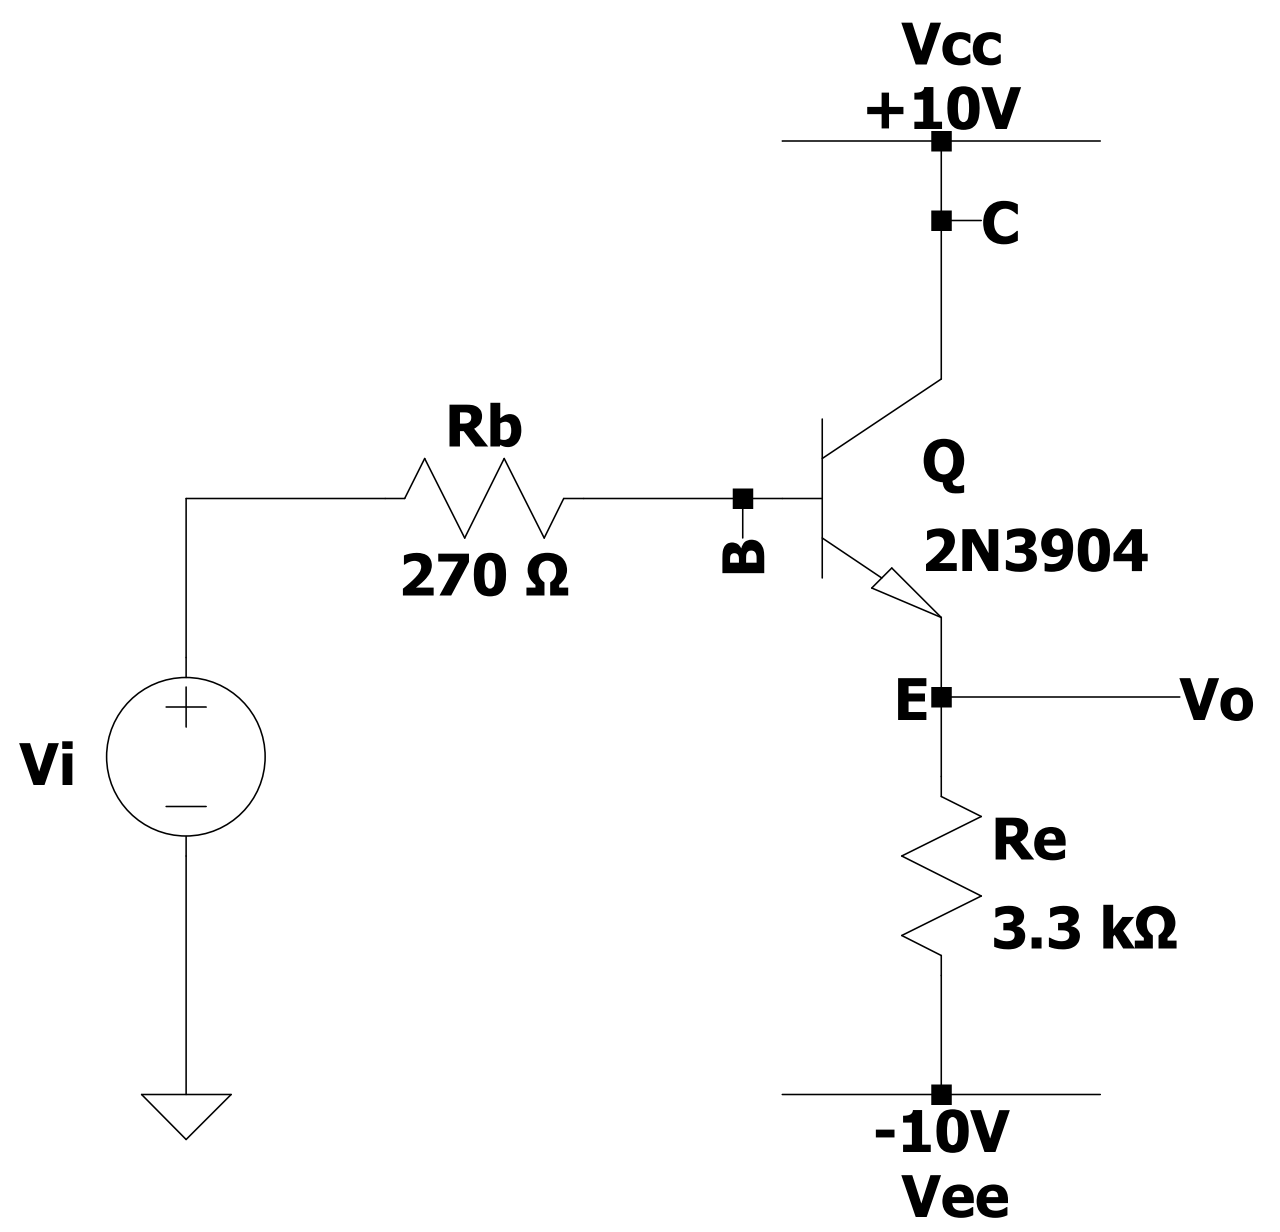
\includegraphics[height=10cm]{immagini/EFv1}
\caption{Schema dell'\textit{Emitter follower} ad alimentazione duale.}
\label{figura:EFv1}
\end{figure}
\subsection{Punto di lavoro} \label{puntolavoroEFv1}
In quest'analisi bisogna spegnere i generatori di segnale e sostituirli con un cortocircuito se sono generatori di tensione, oppure con un circuito aperto se sono generatori di corrente. I condensatori sono sostituiti con un circuito aperto e gli induttori con un cortocircuito. Successivamente si va a determinare la tensione di ogni nodo e la corrente che scorre in ogni ramo. 
\begin{figure}[h]
\centering
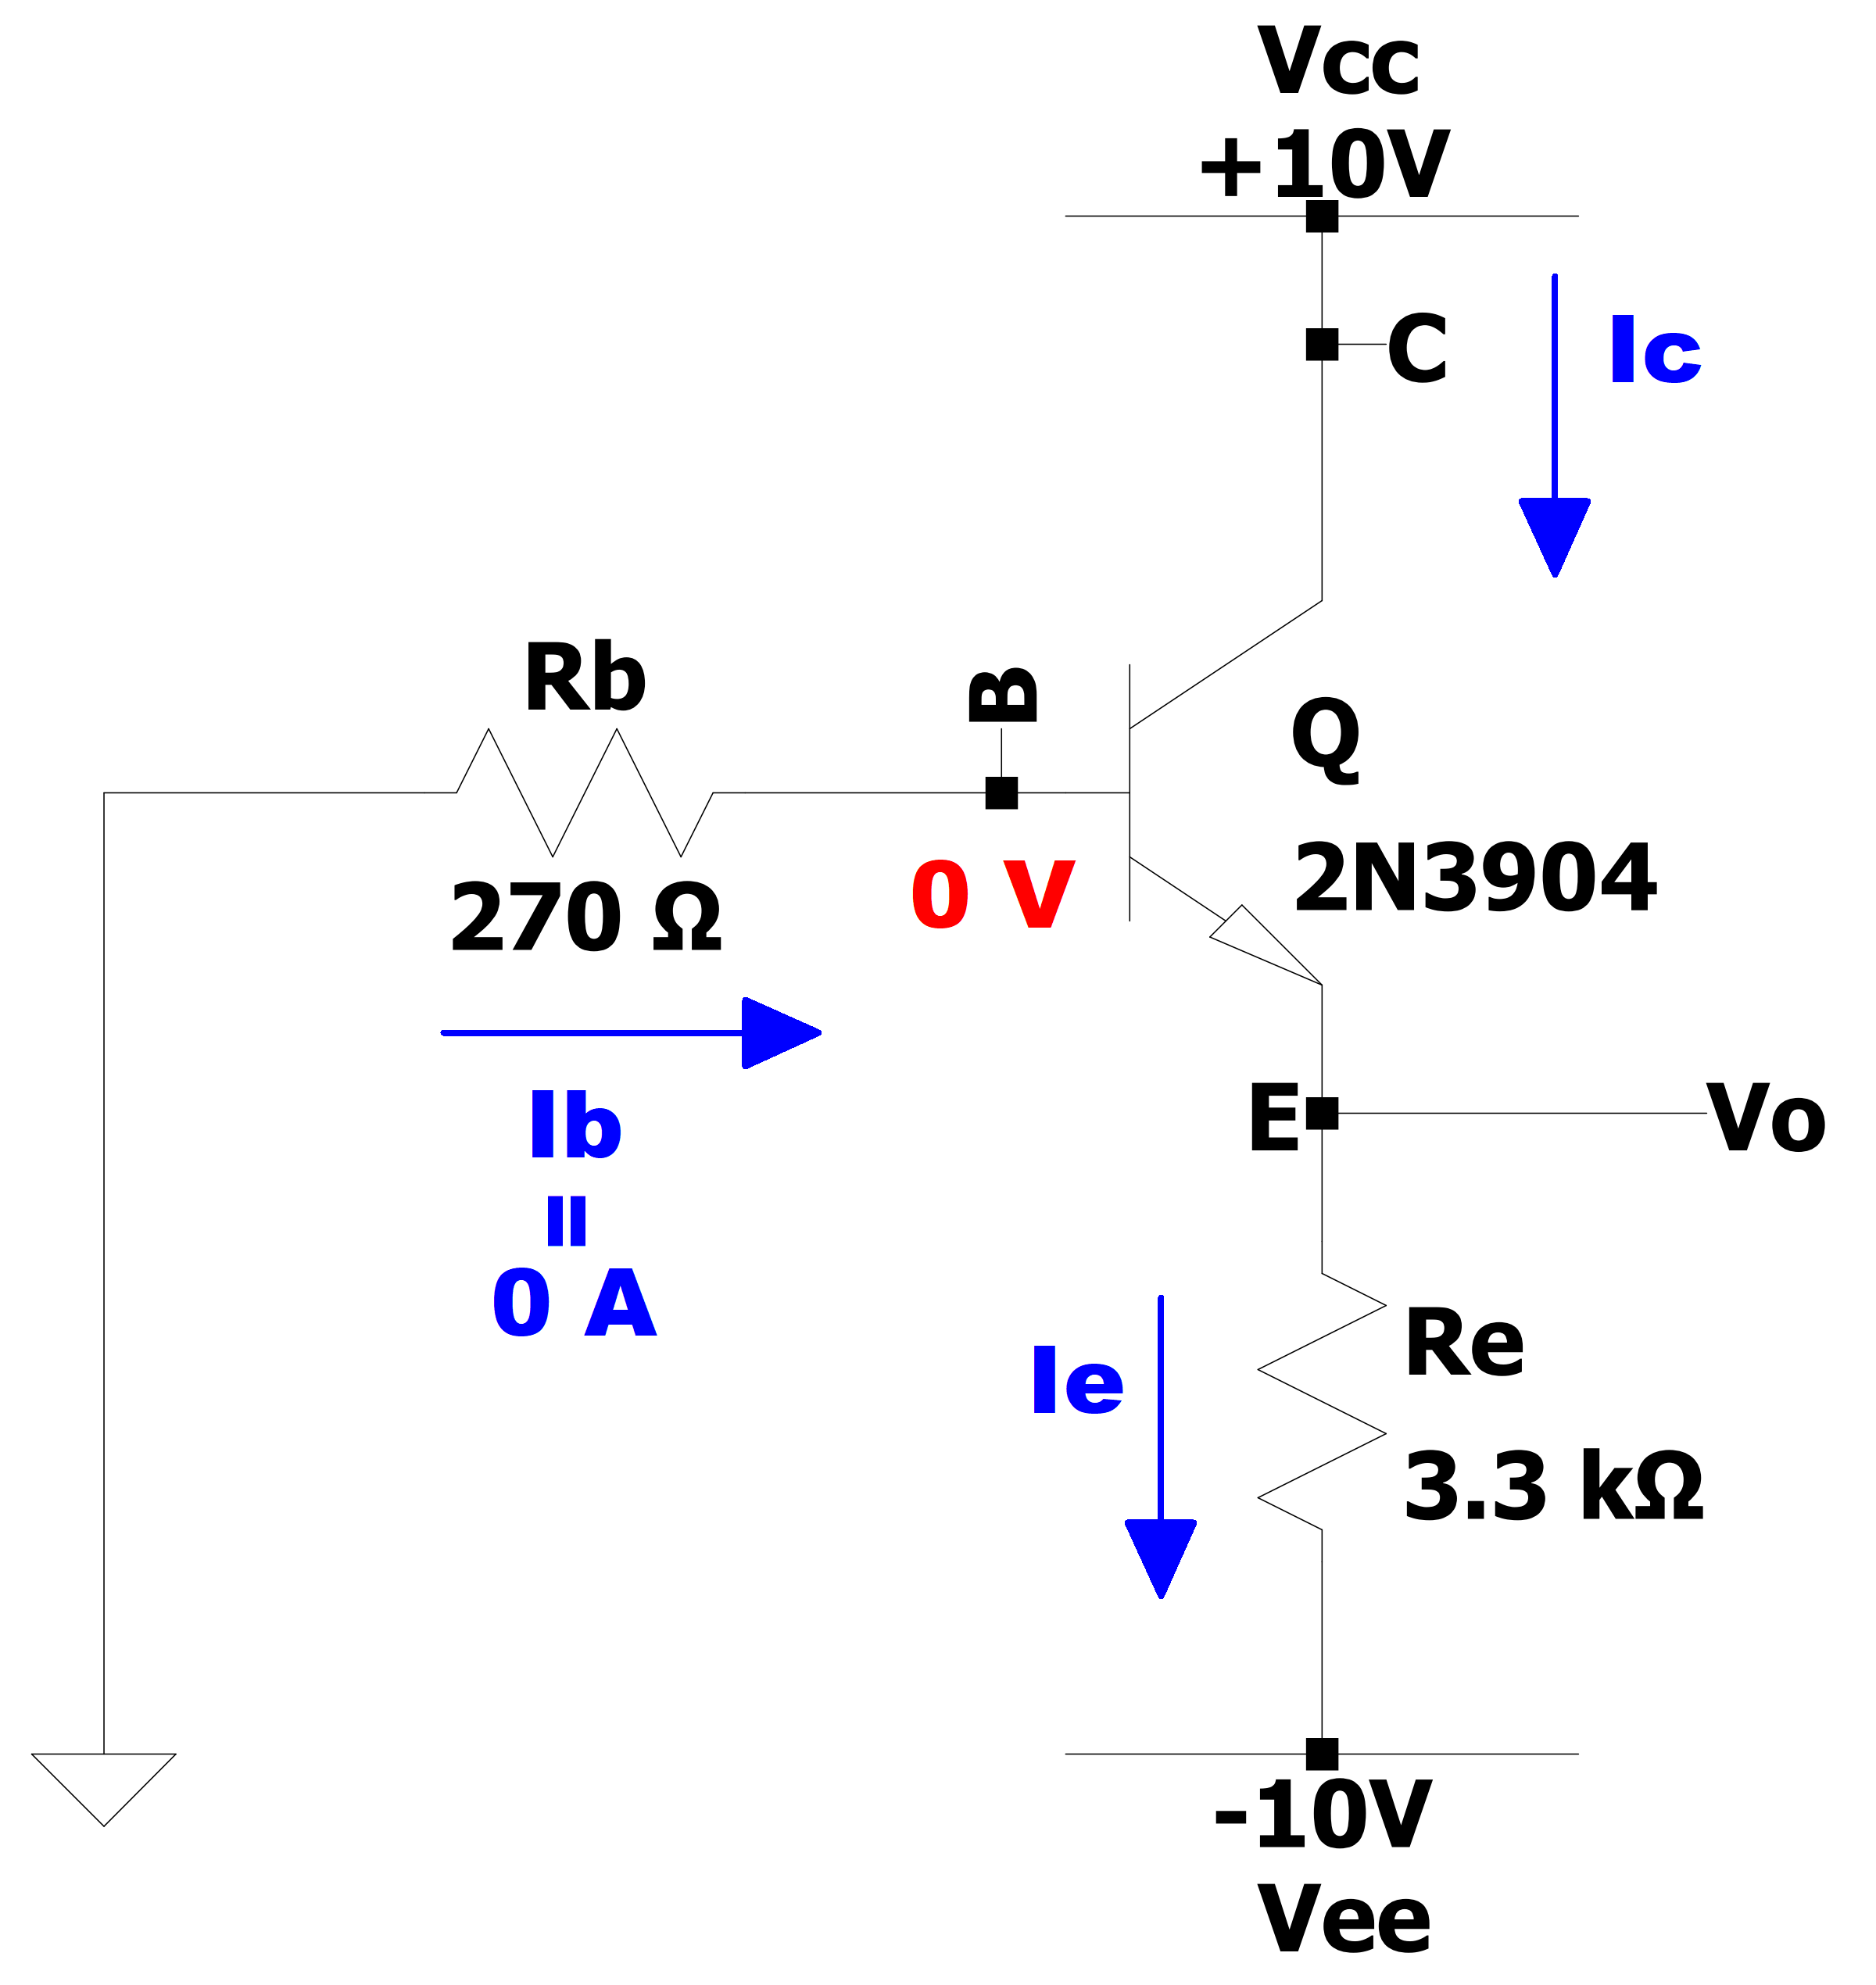
\includegraphics[height=10cm]{immagini/EFv1_pl}
\caption{Punto di lavoro dell'\textit{Emitter follower} ad alimentazione duale.}
\label{figura:EFv1_pl}
\end{figure}
\\Come si vede nell'immagine~\ref{figura:EFv1_pl}, il generatore di segnale $v_{i}$ viene sostituito con un cortocircuito, quindi la resistenza $R_{B}$ si trova fra massa e la base del transistor \textit{Q}. In questo caso non dobbiamo apportare altre modifiche al circuito originale. 
\\Nell'analisi utilizziamo il modello ideale del transistor, perciò assumiamo che $\displaystyle{\beta\rightarrow\infty}$ e che $I_{B}=0A$, di conseguenza la corrente che fluisce nella resistenza è nulla, perciò, per la legge di Ohm, sarà nulla anche la caduta di tensione ai suoi capi, quindi si ricava che $V_{B}=0V$. 
\\Dal bilancio di correnti del  transistor (lo trattiamo come se fosse un nodo) otteniamo che $I_C+I_B=I_E$, ma dato che $I_{B}$ è nulla, allora $I_C=I_E$.
\\Suppondendo che il transistor si trovi in regione attiva diretta, la tensione $V_{BE}$ fra la base e l'emettitore è pari a circa +0.7V perché la giunzione è polarizzata direttamente. Dato che sappiamo che $V_{B}=0V$, possiamo calcolare per differenza $V_{E}$, dunque $V_{E}=0V-0.7V=-0.7V$. Anche $V_o$ sarà pari a questo valore dato che l'uscita viene prelevata all'emettitore.
\\$V_C$ è pari alla tensione di alimentazione positiva, perciò $V_C=V_{CC}=10V$.
Dato che $V_{CB}>0V$, la giunzione base-collettore è polarizzata inversamente, quindi l'ipotesi che il transistor si trovi in regione attiva diretta è verificata. 
\\Ora possiamo calcolare la corrente di emettitore con la legge di Ohm: 
\\[2pt]\indent$\displaystyle{V_E-V_{EE}=R_E\cdot I_E \rightarrow I_E=I_C=\frac{V_E-V_{EE}}{R_E}=\frac{-0.7V-(-10V)}{3.3k\Omega}=2.818mA}$
\\[2pt]Il circuito è ora completamente risolto, come ultima cosa si può calcolare la transconduttanza, visto che ci servirà successivamente per l'analisi di piccolo segnale. La transconduttanza è definita come il rapporto tra la corrente di collettore stazionaria $I_C$ e la tensione termica $V_T$, che a temperatura ambiente vale circa 26mV. 
\\[2pt]In formule: $\displaystyle{g_m=\frac{I_C}{\Phi_T}=\frac{2.818mA}{26mV}=0.108 \frac{A}{V}}$.
\\[3pt]In tabella \ref{table:EFv1_pl} sono riassunte tutte le grandezze ricavate dal punto di lavoro. 
\begin{table}[h]
	\centering
	\begin{tabular}{|c|c|c|c|c|c|c|}
		\hline
		\textbf{V\ped{B}[V]} & \textbf{V\ped{C}[V]} & \textbf{V\ped{E}[V]} & \textbf{I\ped{B}[A]} & \textbf{I\ped{E}[mA]} & \textbf{I\ped{C}[mA]} & \textbf{g\ped{m}[A/V]} \\ 
		\hline
		0 & 10 & -0.7 & 0 & 2.818 & 2.818 & 0.108\\ 
		\hline
	\end{tabular}
\caption{Riassunto delle grandezze ricavate dal punto di lavoro del circuito.}
\label{table:EFv1_pl}
\end{table}
\subsection{Analisi di piccolo segnale} \label{piccolosegnaleEFv1}
Nell'analisi di piccolo segnale bisogna spegnere i generatori di grandezze continue e sostituirli con un cortocircuito se sono generatori di tensione, oppure con un circuito aperto se sono generatori di corrente. Per analisi approssimate, i condensatori sono sostituiti con un cortocircuito e gli induttori con un circuito aperto; per analisi più accurate, invece, non vengono sostituiti e si utilizza la loro impedenza per risolvere il circuito. Infine, i transistor vengono sostituiti con il loro modello per piccolo segnale. Successivamente si va a determinare la tensione di ogni nodo e la corrente che scorre in ogni ramo, esattamente come avveniva per l'analisi del punto di lavoro. 
\begin{figure}[h]
\centering
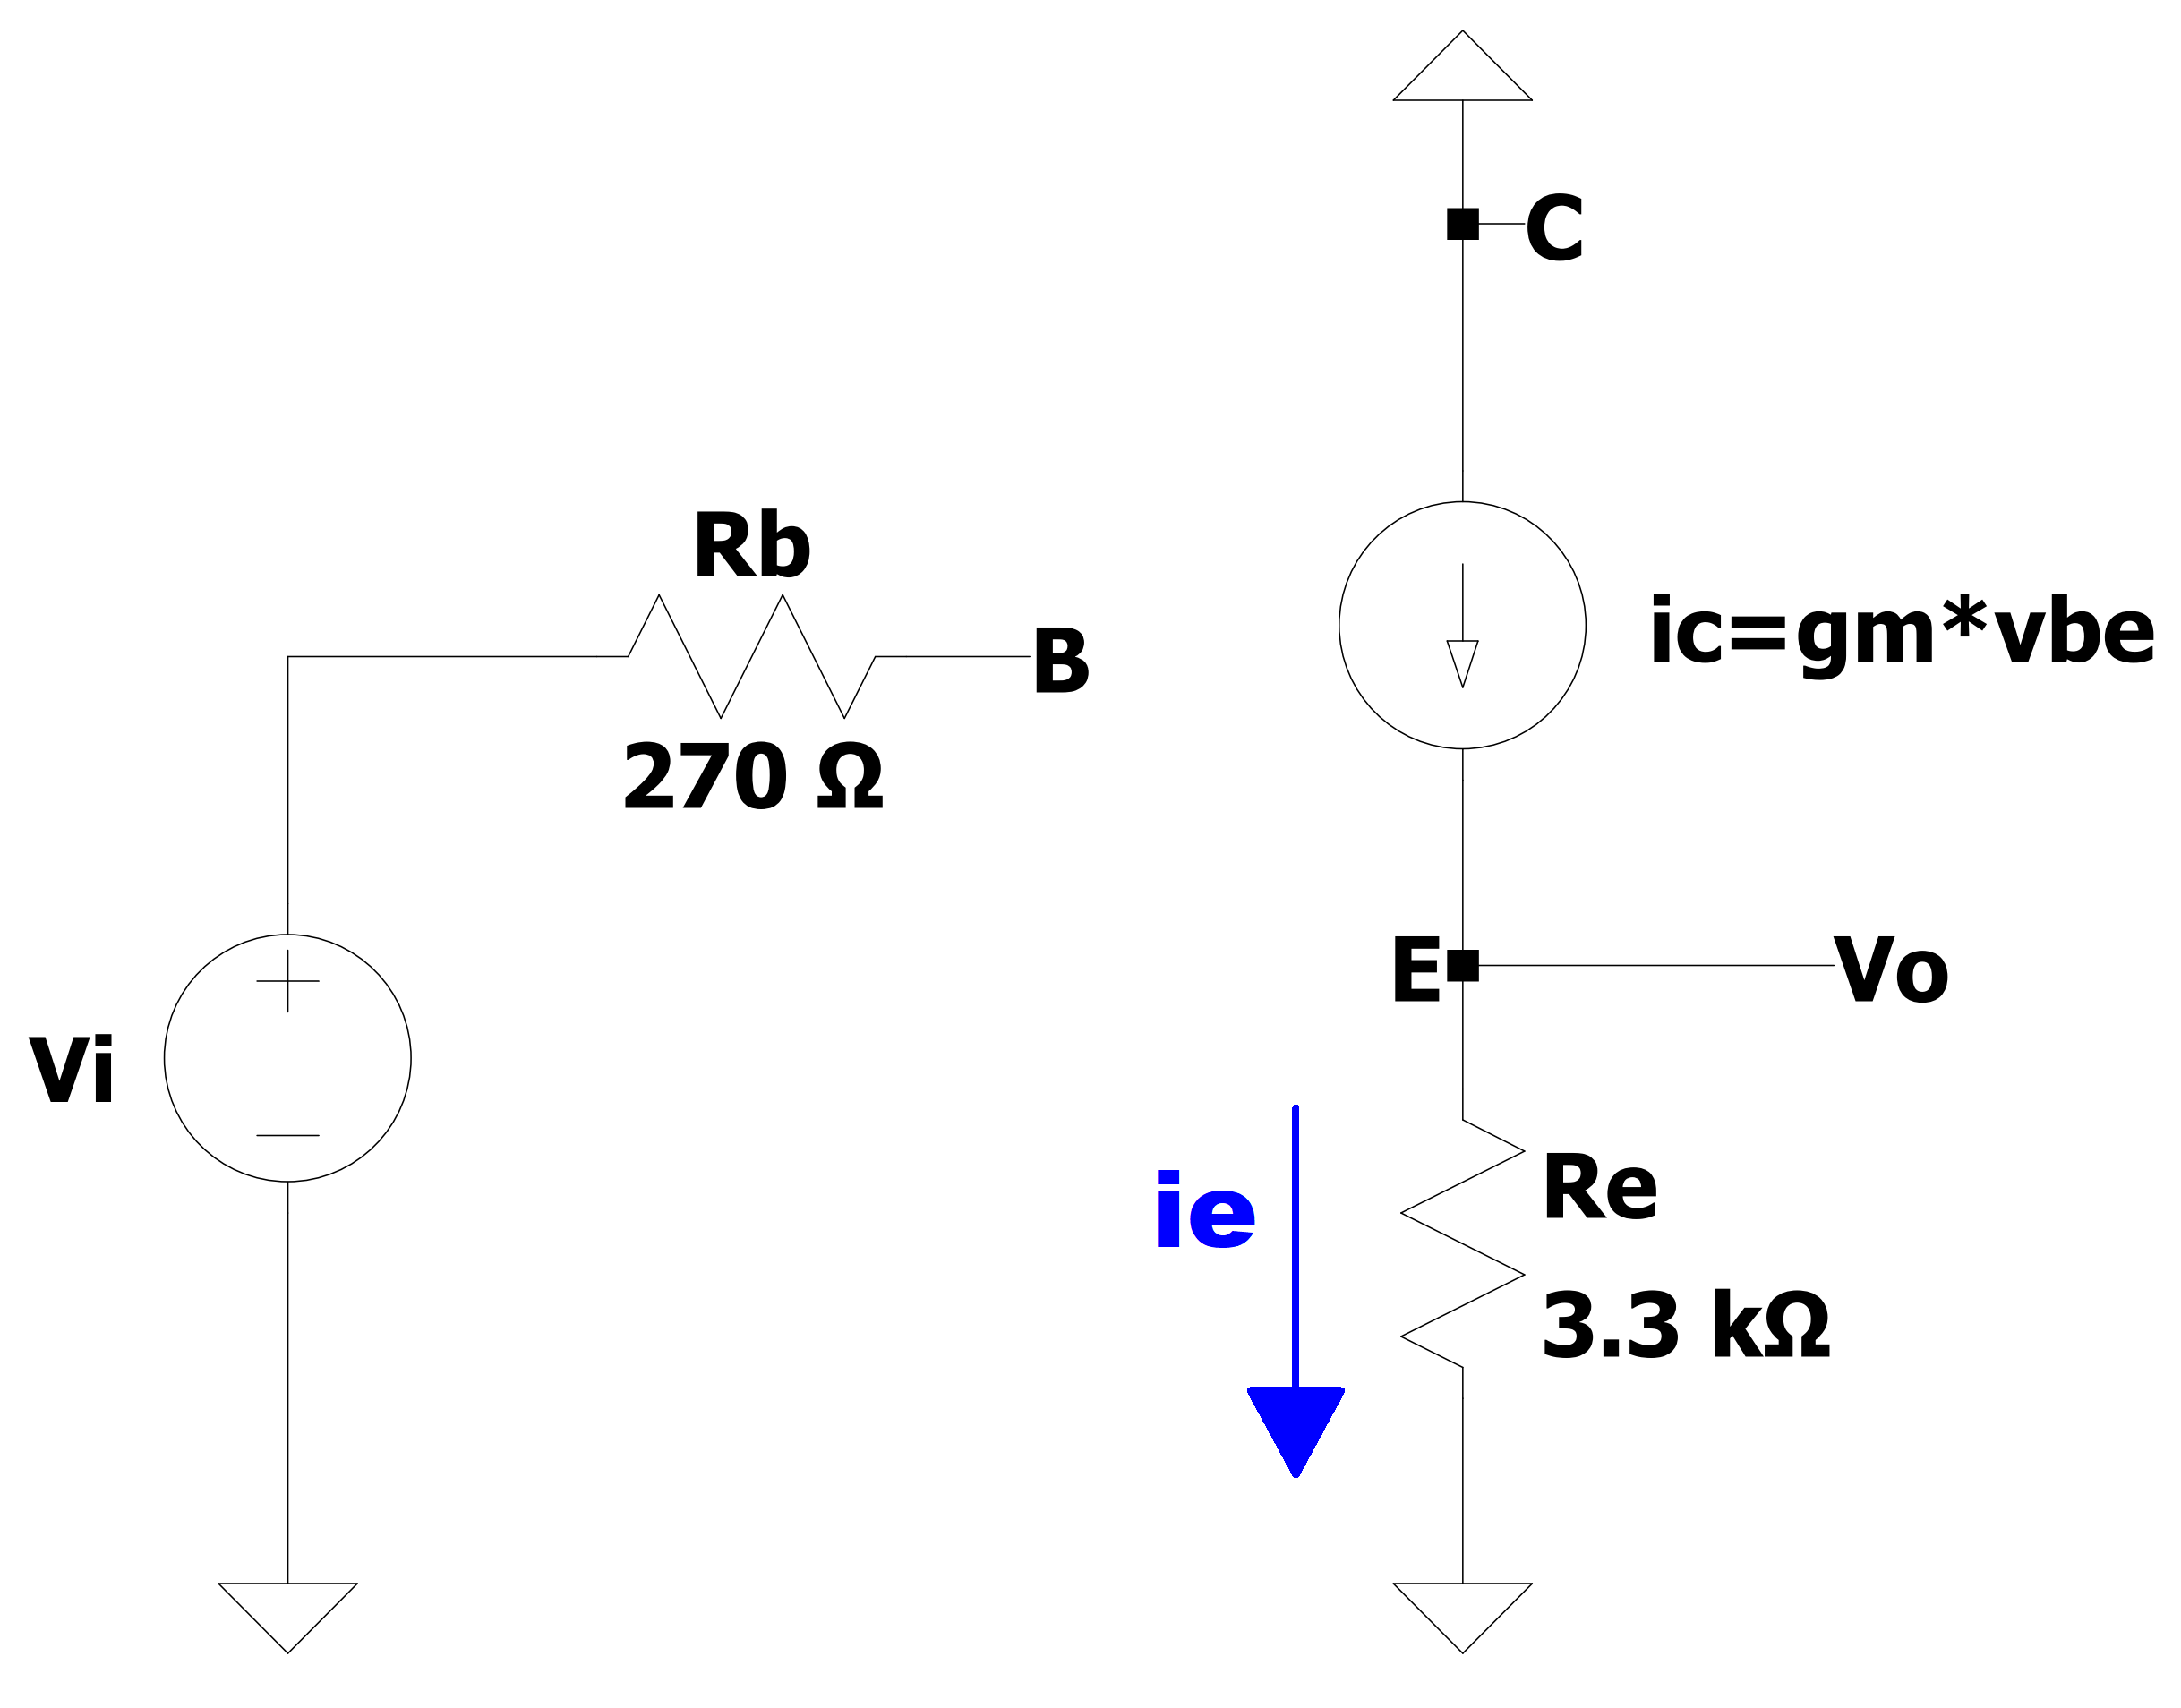
\includegraphics[height=9.6cm]{immagini/EFv1_ps}
\caption{Analisi di piccolo segnale dell'\textit{Emitter follower} ad alimentazione duale.}
\label{figura:EFv1_ps}
\end{figure}
\\Come si può notare dalla figura~\ref{figura:EFv1_ps}, il BJT viene sostituito con il modello per piccolo segnale a bassa frequenza, quindi il terminale di base risulta isolato dal collettore e dall'emettitore; invece, questi due terminali sono collegati attraverso un generatore di corrente ideale di valore pari al prodotto fra la transconduttanza $g_m$ e la tensione $v_{BE}$.
\\Dato che la base del transistor è isolata, nel circuito di sinistra non circola corrente, perciò non c'è caduta di tensione sulla resistenza $R_B$, quindi la tensione $v_B$ risulta pari alla tensione applicata in ingresso con il generatore $v_i$.
\\Abbiamo già detto che $i_C=g_m\cdot v_{BE} = g_m(v_B-v_E) $. Ma dato che $v_B=v_i$ e $v_E=v_o$, la formula precedente per il calcolo della corrente di collettore si può riscrivere come $i_C=g_m(v_i-v_o)$.
\\[2pt]Ricaviamo $i_E$ con la legge di Ohm: 
$\displaystyle{i_E=\frac{v_E-0V}{R_E}=\frac{v_o}{R_E}}$.
\\[2 pt] Dal bilancio delle correnti al nodo E otteniamo che $i_C=i_E$. Sostituendo alle due correnti le espressioni ricavate ai punti precedenti possiamo scrivere la seguente eqauazione:
\\[2pt]\indent $\displaystyle{g_m(v_i-v_o)=\frac{v_o}{R_E}}$.
\\[2pt] A questo punto possiamo ricavare la funzione di trasferimento del circuito manipolando l'espressione ottenuta in precedenza. Questa risulta:
\\[2pt]\indent $\displaystyle{\frac{v_o}{v_i}=\frac{g_mR_E}{1+g_mR_E}\simeq1}$ per $g_mR_E\gg 1$. 
\\[2pt]Allora, si può dire che $v_o=v_i$, ovvero il circuito si comporta come un buffer, come si era già accennato nell'introduzione del circuito (sezione \ref{introEFv1}).
\subsection{Componenti, strumenti e misure} 
Il circuito, mostrato in figura \ref{figura:fotoEFv1}, è stato realizzato su una breadboard utilizzando questi componenti:
\begin{itemize}
\item transistor bipolare NPN 2N3904;
\item una resistenza da \SI{270}{\ohm} per $R_B$;
\item due resistenze, una da \SI{1.5}{k\ohm} ($R_{E_1}$) ed una da \SI{1.8}{k\ohm} ($R_{E_2}$) connesse in serie, per realizzare la resistenza $R_E$ da \SI{3.3}{k\ohm}.
\end{itemize}
\begin{figure}[h]
\centering
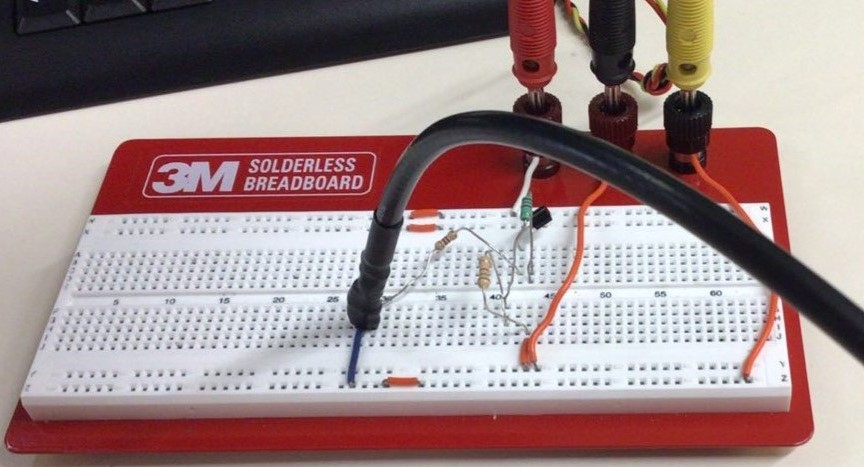
\includegraphics[height=6.6cm]{immagini/fotoEFv1}
\caption{Fotografia del circuito \textit{Emitter follower} ad alimentazione duale realizzato in laboratorio.}
\label{figura:fotoEFv1}
\end{figure}
Per le misure e le analisi, sono stati utilizzati i seguenti strumenti:
\begin{itemize}
\item alimentatore da banco, con alimentazione positiva impostata a 10V ed alimentazione negativa a -10V, entrambe con limite in corrente di 50mA;
\item generatore di forme d'onda;
\item multimetro da banco;
\item oscilloscopio a due canali.
\end{itemize}
Per prima cosa, con il multimetro si sono misurati i valori delle resistenze ed i valori delle tensioni delle giunzioni p-n del transistor (tensione \textit{base-emettitore} e tensione \textit{base-collettore}). I valori ottenuti sono mostrati in tabella \ref{table:EFv1_comp}.
\begin{table}[h]
	\centering
	\begin{tabular}{|c|c|c|}
	\cline{2-3} 
	\multicolumn{1}{c|}{} & \textbf{Valore nominale} & \textbf{Valore misurato}\\ 
		%\hline
		%{} & \textbf{Valore nominale} & \textbf{Valore misurato} \\ 
		\hline
		$\mathbf{R_B}$ & \SI{270}{\ohm} & \SI{271}{\ohm} \\ 
		\hline
		$\mathbf{R_{E_1}}$& \SI{1.5}{k\ohm} & \SI{1.448}{k\ohm} \\ 
		\hline
		$\mathbf{R_{E_2}}$& \SI{1.8}{k\ohm} & \SI{1.788}{k\ohm} \\ 
		\hline
		$\mathbf{V_{BE}}$& $\mathrm{ \simeq0.7V}$ & 0.699V \\ 
		\hline
		$\mathbf{V_{BC}}$& $\mathrm{ \simeq0.7V}$  & 0.659V \\ 
		\hline
	\end{tabular}
	
\caption{Grandezze misurate prima di realizzare il circuito.}
\label{table:EFv1_comp}
\end{table}
\\Le due giunzioni p-n hanno valori di tensione diversi, questo è dovuto alla tecnologia di realizzazione del BJT: essendo un dispositivo planare, le due giunzioni hanno lunghezza diversa, di conseguenza anche il loro valore di tensione sarà diverso. Il valore totale della resistenza $R_E$ è pari a \SI{3.236}{k\ohm}, poco meno del 2\% rispetto al suo valore nominale che è \SI{3.3}{k\ohm}.
\\\indent Dopo aver posizionato tutti i componenti sulla breadboard, è stato fatto lo studio del punto di lavoro del circuito. Non è stato applicato il segnale e il terminale della resistenza $R_B$ non connesso alla base del transistor è stato collegato a massa. Il circuito risultante è mostrato in figura \ref{figura:fotoEFv1_pl}.
\begin{figure}[h]
\centering
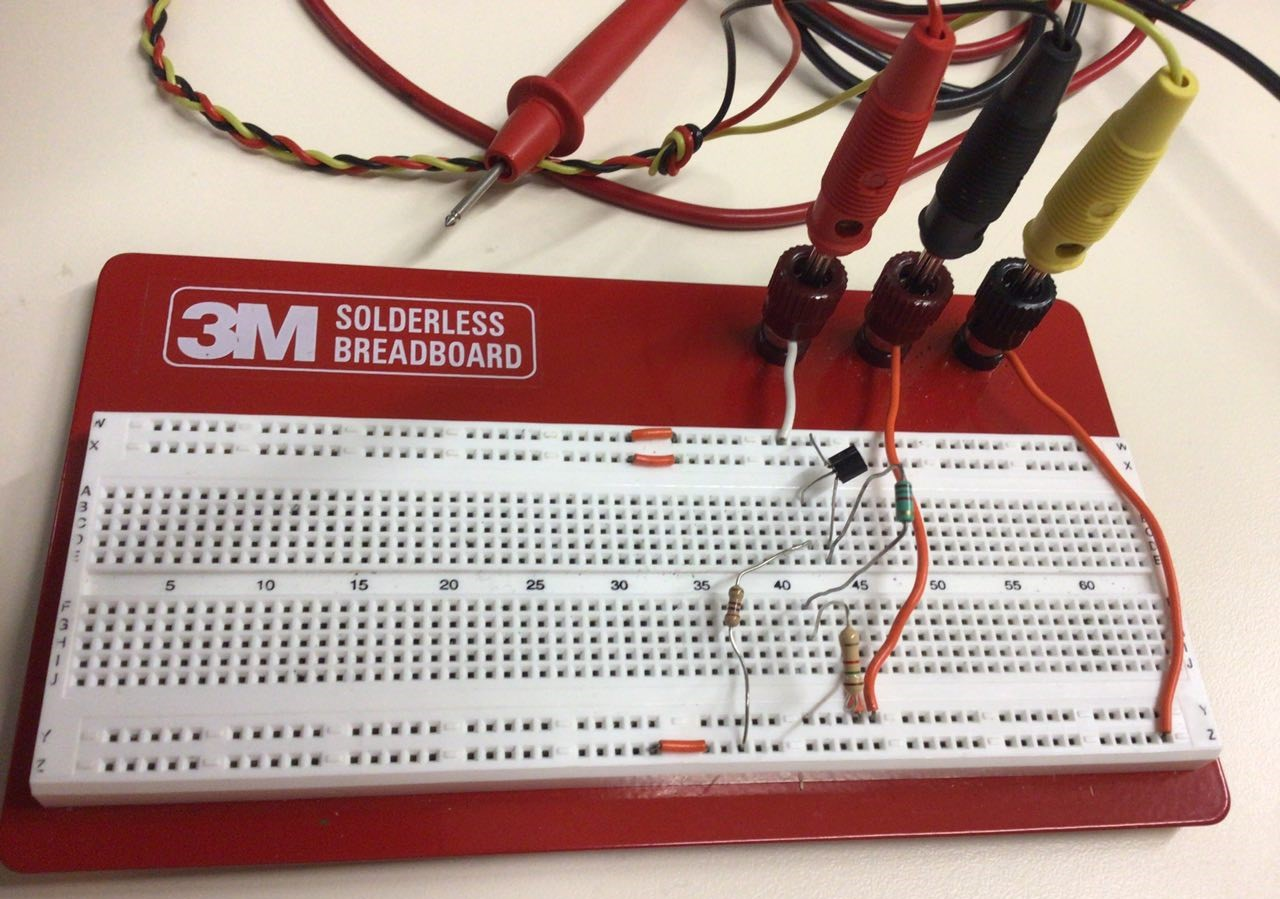
\includegraphics[height=7.3cm]{immagini/fotoEFv1_pl}
\caption{Fotografia del circuito \textit{Emitter follower} con le connessioni per lo studio del punto di lavoro.}
\label{figura:fotoEFv1_pl}
\end{figure}
\\Le tensioni sono state misurate con il multimetro da banco, le correnti di base e di emettitore sono state ricavate utilizzando la legge di Ohm, mentre la corrente di collettore è stata calcolata per differenza dalle altre due correnti. I risultati sono mostrati in tabella \ref{table:EFv1_pl_mis}. 
\begin{table}[h]
	\centering
	\begin{tabular}{|c|c|c|c|c|c|c|}
		\hline
		\textbf{V\ped{B}[mV]} & \textbf{V\ped{C}[V]} & \textbf{V\ped{E}[V]} & \textbf{I\ped{B}[mA]} & \textbf{I\ped{E}[mA]} & \textbf{I\ped{C}[mA]} & \textbf{g\ped{m}[A/V]} \\ 
		\hline
		-3.515 & 10.000 & -0.687 & 0.013 & 2.878 & 2.865 & 0.108\\ 
		\hline
	\end{tabular}
\caption{Grandezze misurate dallo studio del punto di lavoro del circuito.}
\label{table:EFv1_pl_mis}
\end{table}
\\I valori ottenuti sono confrontabili con i risultati teorici calcolati nella sezione \ref{puntolavoroEFv1}. La differenza principale è che sia $V_B$ che $I_B$ non sono nulle, anche se il loro valore (in modulo) è molto piccolo. In particolare, dato che la corrente $I_B$ è piccola, l'approssimazione adottata nello studio teorico del circuito di trascurarla è ragionevole. 
\\\indent Dopo lo studio del punto di lavoro del circuito, è stato applicato in ingresso il segnale collegando con un cavo BNC il generatore di forme d'onda al circuito. Il circuito risultante è quello già mostrato in figura \ref{figura:fotoEFv1}. La forma d'onda utilizzata è una sinusoide con tensione picco-picco $V_{PP}$ di 2V e frequenza $f$ pari a \SI{1}{k\hertz}. 
\\\indent Per visualizzare graficamente la tensione in ingresso e la tensione in uscita è stato utilizzato l'oscilloscopio. Entrambe le sonde sono state collegate a massa con il coccodrillo, la punta di una sonda è stata collegata alla base del transistor (canale 1, traccia gialla) mentre la punta dell'altra sonda è stata collegata all'emettitore (canale 2, traccia azzurra). Il grafico è visibile in figura \ref{figura:oscillo1}.
\begin{figure}[h]
\centering
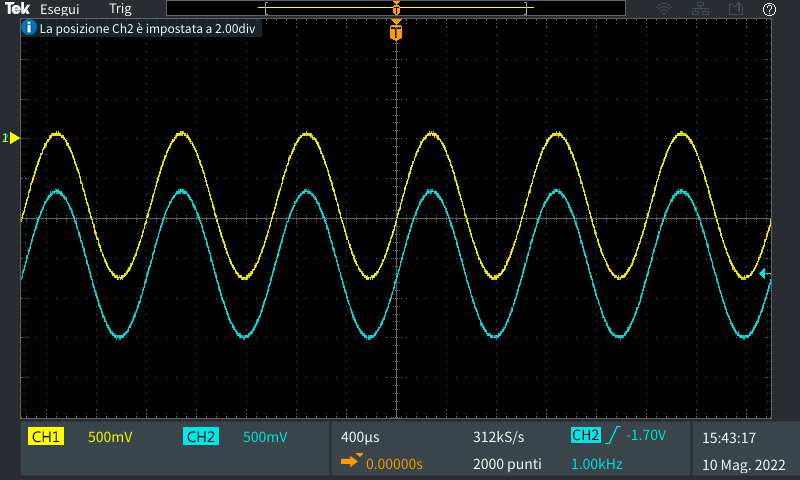
\includegraphics[height=7cm]{immagini/oscillo1}
\caption{Grafico della tensione in ingresso (CH1) ed in uscita (CH2) al circuito, accoppiate in DC.}
\label{figura:oscillo1}
\end{figure}
\\
Com'è possibile vedere dal grafico, il guadagno del circuito è unitario perché entrambe le sinusoidi hanno la stessa ampiezza. La tensione applicata in ingresso la misuriamo in uscita con una differenza di circa 0.7V, che è la caduta di tensione data dalla giunzione p-n fra base ed emettitore. I due segnali sono in fase. 
\\\indent In realtà, il guadagno del circuito non è esattamente unitario e nemmeno lo sfasamento, o offset, è proprio nullo, come invece sembrerebbe dal grafico precedente. La tensione in uscita è legata alla tensione in ingresso da una relazione del tipo $y=a+bx$, dove $y$ è la tensione in uscita, $x$ la tensione in ingresso, $a$ l'offset e $b$ il guadagno del circuito. Per ricavare il valore dei parametri $a$ e $b$ sono state applicate in ingresso al circuito diverse sinusoidi, tutte di frequenza \SI {1}{k\hertz} ma di ampiezza variabile. La tensione picco-picco è infatti stata variare da 0.5V a 5.0V con step di 0.5V. Successivamente, con l'oscilloscopio, si sono misurati i valori di tensione picco-picco in ingresso, $V_{PP_i}$, e in uscita, $V_{PP_o}$. 
\\\indent Per ridurre l'effetto dei disturbi e del rumore sulle misure, i segnali sono stati filtrati con un passa-basso con frequenza di taglio di \SI{20}{M\hertz}, poi sono stati mediati utilizzando 16 acquisizioni. Facendo così, il valore misurato dall'oscilloscopio risulta molto più stabile. Le misure sono riportate in tabella \ref{table:tabgrafico}.
\begin{table}[h]
	\centering
	\begin{tabular}{|c|c|}
		\hline
		$\mathbf{V_{PP_i}[V]}$ & $\mathbf{V_{PP_o}[V]}$\\ 
		\hline
		0.503 & 0.505 \\
		\hline
		1.000 & 1.006 \\
		\hline
		1.497 & 1.506 \\
		\hline
		1.989 & 2.002 \\
		\hline
		2.486 & 2.502 \\
		\hline
		2.978 & 3.001 \\
		\hline
		3.473 & 3.496 \\
		\hline
		3.965 & 3.993 \\
		\hline
		4.461 & 4.497 \\
		\hline
		4.951 & 4.985 \\
		\hline
	\end{tabular}
\caption{Valori della tensione picco-picco in ingresso e in uscita al circuito.}
\label{table:tabgrafico}
\end{table}
\\I dati della tabella precedente sono stati elaborati su MATLAB per ricavare la retta di regressione che ci permette di stimare i valori di $a$ e $b$. Nel grafico seguente, la figura \ref{figura:graficoEFv1}, si riportano le misure, la retta interpolata e la retta teorica. 
\begin{figure}[h]
\centering
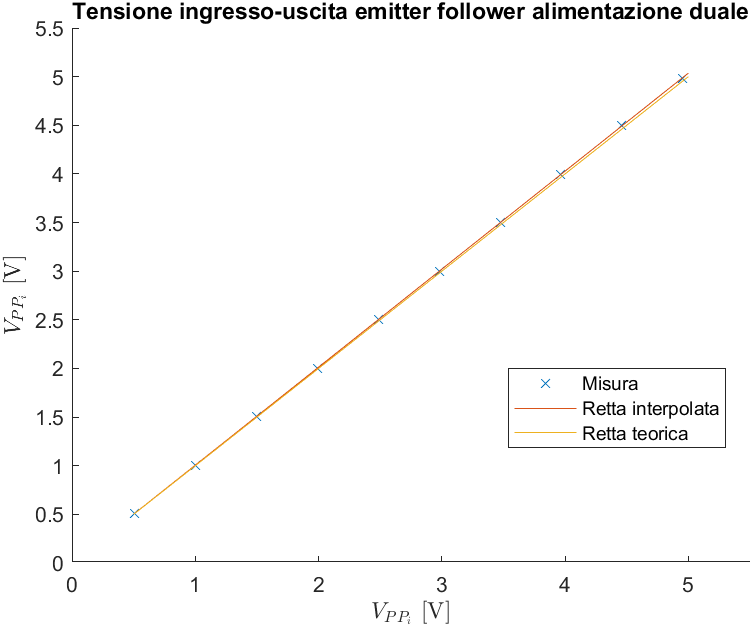
\includegraphics[height=7cm]{immagini/graficoEFv1}
\caption{Confronto grafico fra la tensione ingresso-uscita interpolata e quella teorica.}
\label{figura:graficoEFv1}
\end{figure}
\\L'equazione della retta interpolata è: $y=-0.0020949+1.0077x$. Il risultato è chiaramente in disaccordo con la teoria, perché sebbene il guadagno è molto prossimo all'unità, non può essere maggiore, perché questo significherebbe che il circuito eroga più energia rispetto a quella fornita in ingresso. \\\\ Infatti, il circuito ha una resistenza d'uscita $r_{out}$ di valore circa pari a:
\\[2pt]\indent$\displaystyle{r_{out}\simeq\frac{1}{g_m}}$ \indent con  $\displaystyle{g_m=\frac{I_C}{V_T}}$
\\[2pt]La funzione di trasferimento di conseguenza è leggermente diversa da quella ottenuta alla fine della sezione \ref{piccolosegnaleEFv1}, ed è uguale a:
\\[2pt]\indent $\displaystyle{\frac{v_o}{v_i}=\frac{R_E}{r_{out}+R_E}}$
\\[2pt]da cui risulta evidente che il guadagno non può essere sicuramente maggiore di uno. Il motivo di questo risultato anomalo può essere dovuto alla regolazione non sufficientemente precisa della capacità di compensazione della sonda collegata al secondo canale dell'oscilloscopio.
\section{Seconda versione} % alimentazione singola 
\label{EFv2cap}
Nel circuito appena realizzato abbiamo usato due alimentazioni, una positiva ed una negativa. Se il circuito non fosse alimentato con l'alimentatore da banco, per farlo funzionare servirebbero due batterie da 10V. Adottando alcuni accorgimenti, si può modificare il circuito discusso prima per fare in modo che funzioni con una sola alimentazione, l'altra viene collegata a massa. Siamo perciò passati a studiare l'\textit{Emitter follower} ad alimentazione singola. Il circuito di partenza è mostrato in figura \ref{figura:EFv2_1}, è lo stesso circuito di figura \ref{figura:EFv1} ma al posto dell'alimentazione negativa troviamo la massa. Trascuriamo per ora i valori delle resistenze. Verrano man mano discusse le modifiche e le eventuali problematiche che si riscontreranno per arrivare alla versione finale del circuito.
\begin{figure}[h]
\centering
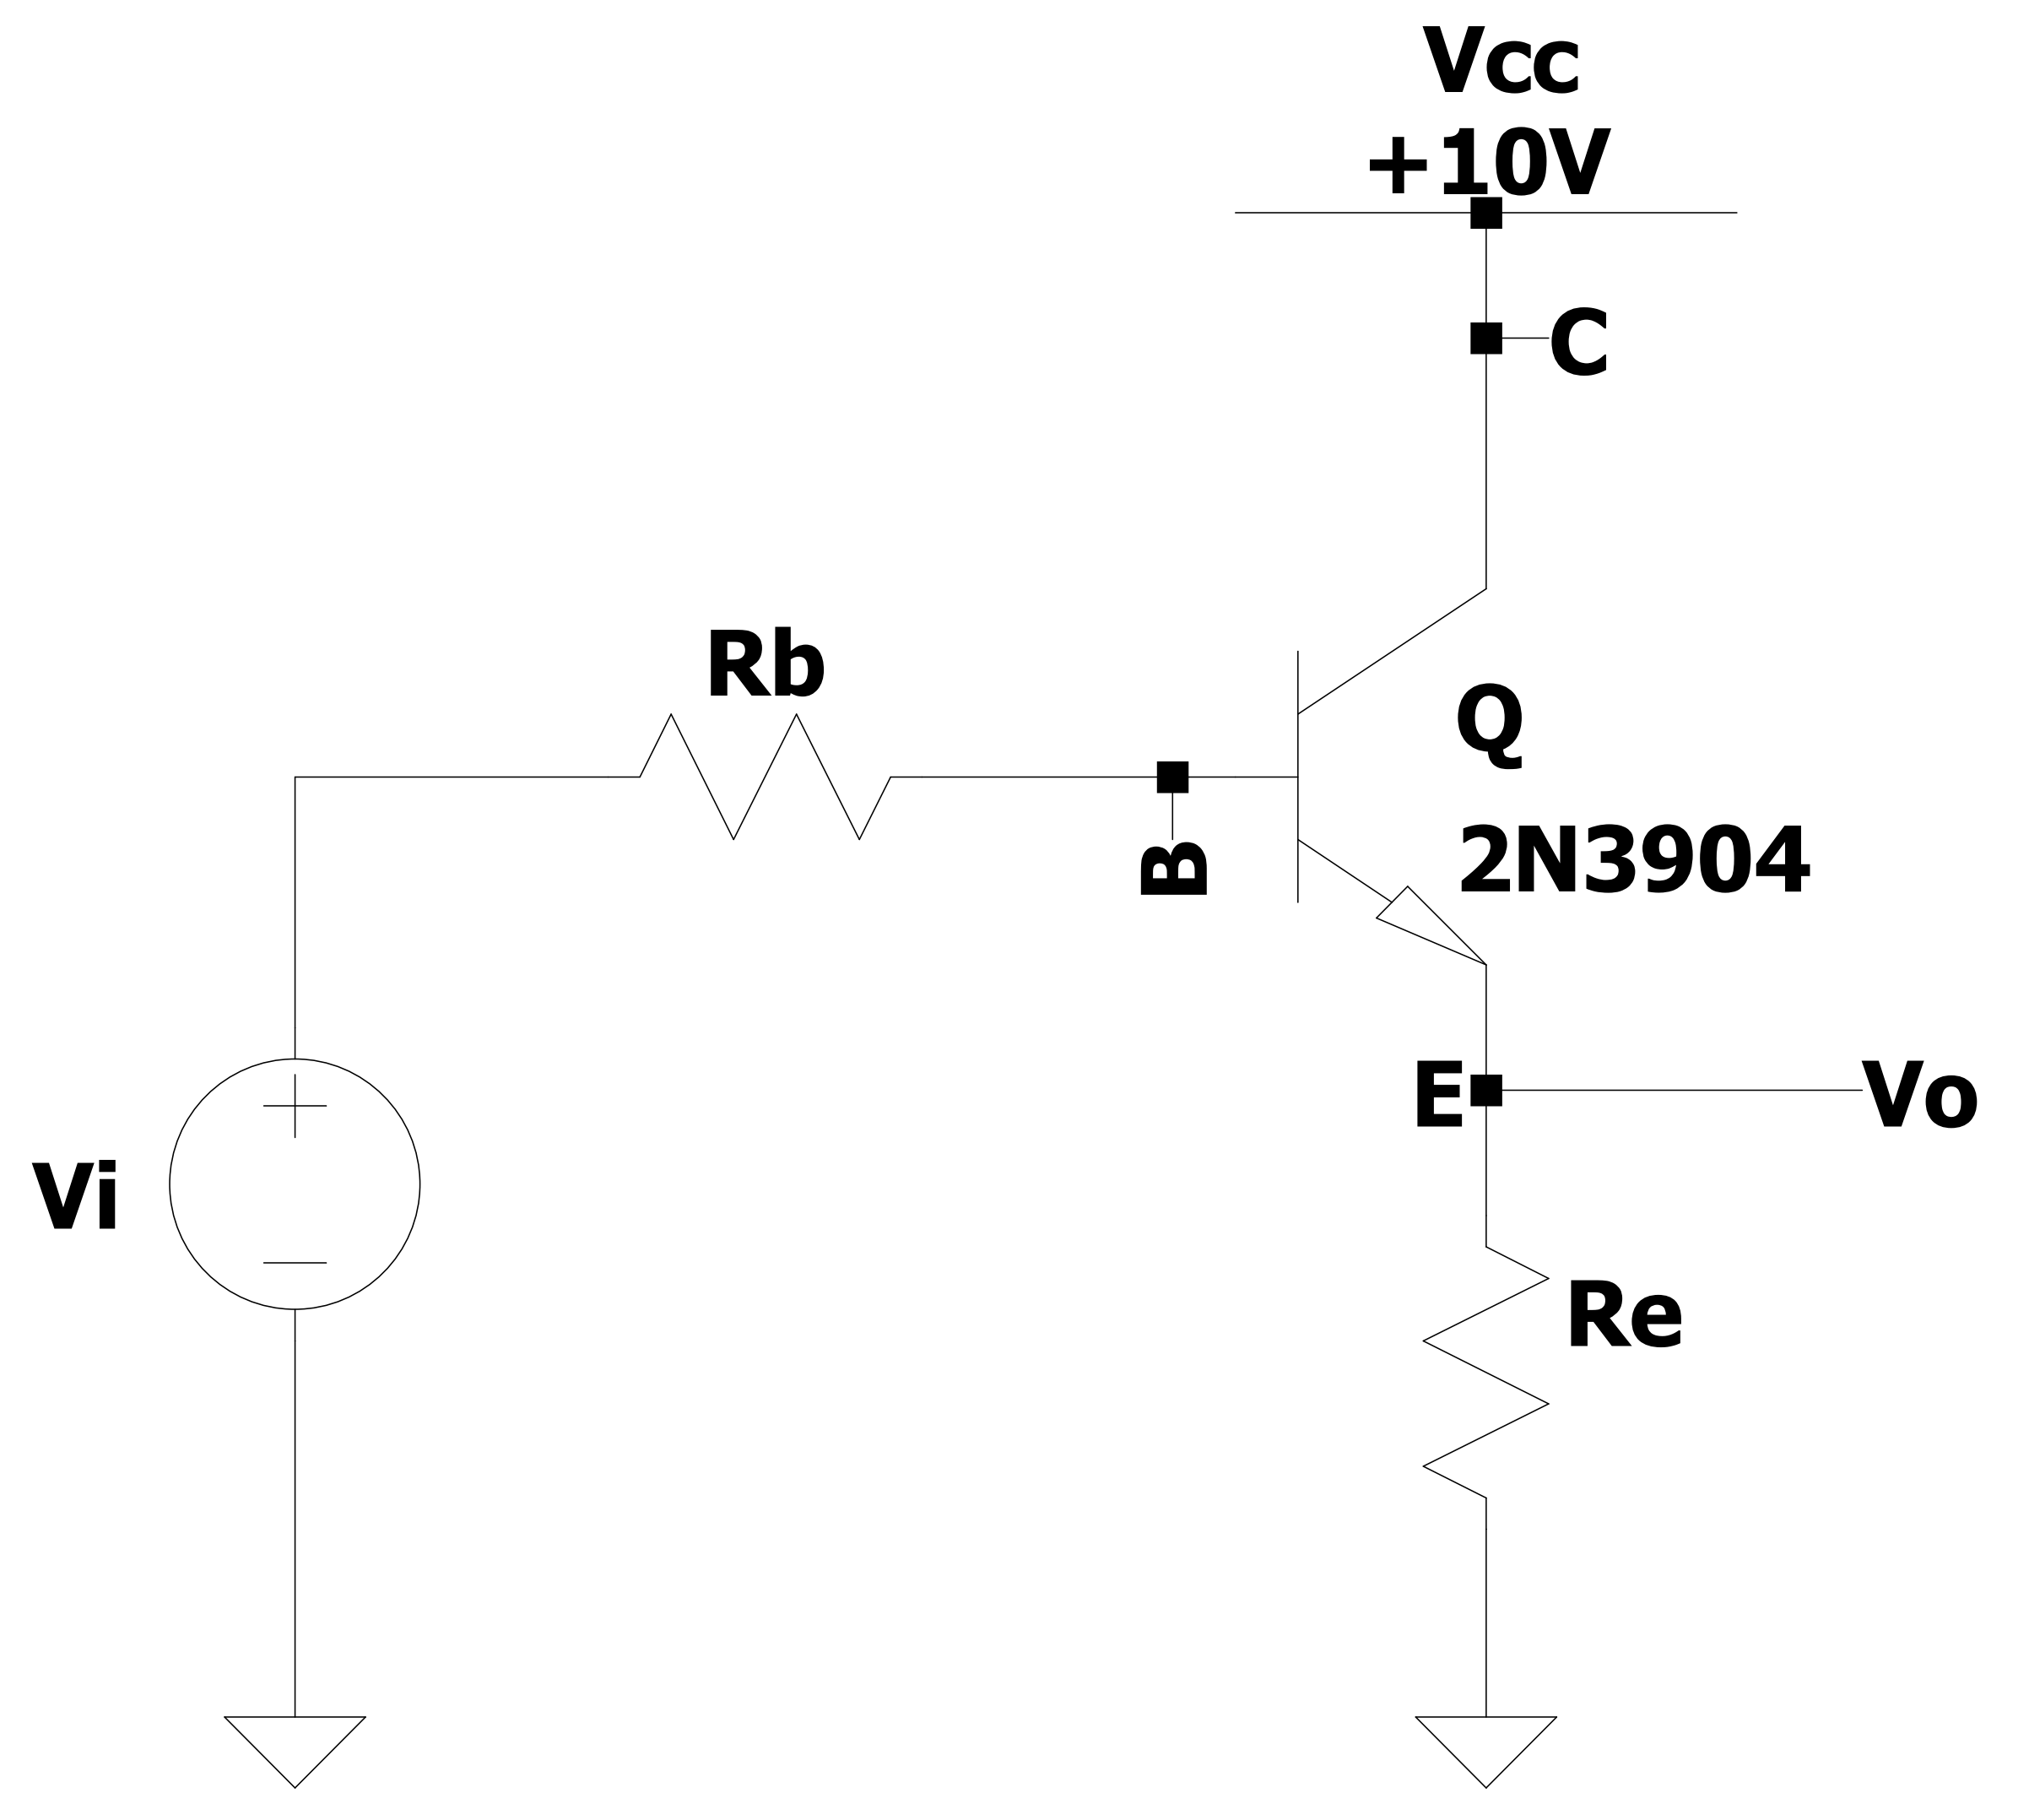
\includegraphics[height=10cm]{immagini/EFv2_1}
\caption{Schema di partenza dell'\textit{Emitter follower} ad alimentazione singola.}
\label{figura:EFv2_1}
\end{figure}
\subsection{Punto di lavoro} % versione base + versione partitore + versione condensatore
Per quest'analisi è sufficiente sostituire il generatore di tensione $v_i$ con un cortocircuito, esattamente come per l'\textit{Emitter follower} ad alimentazione duale. Lo schema risultante è riportato in figura \ref{figura:EFv2_1_pl}.
\begin{figure}[h]
\centering
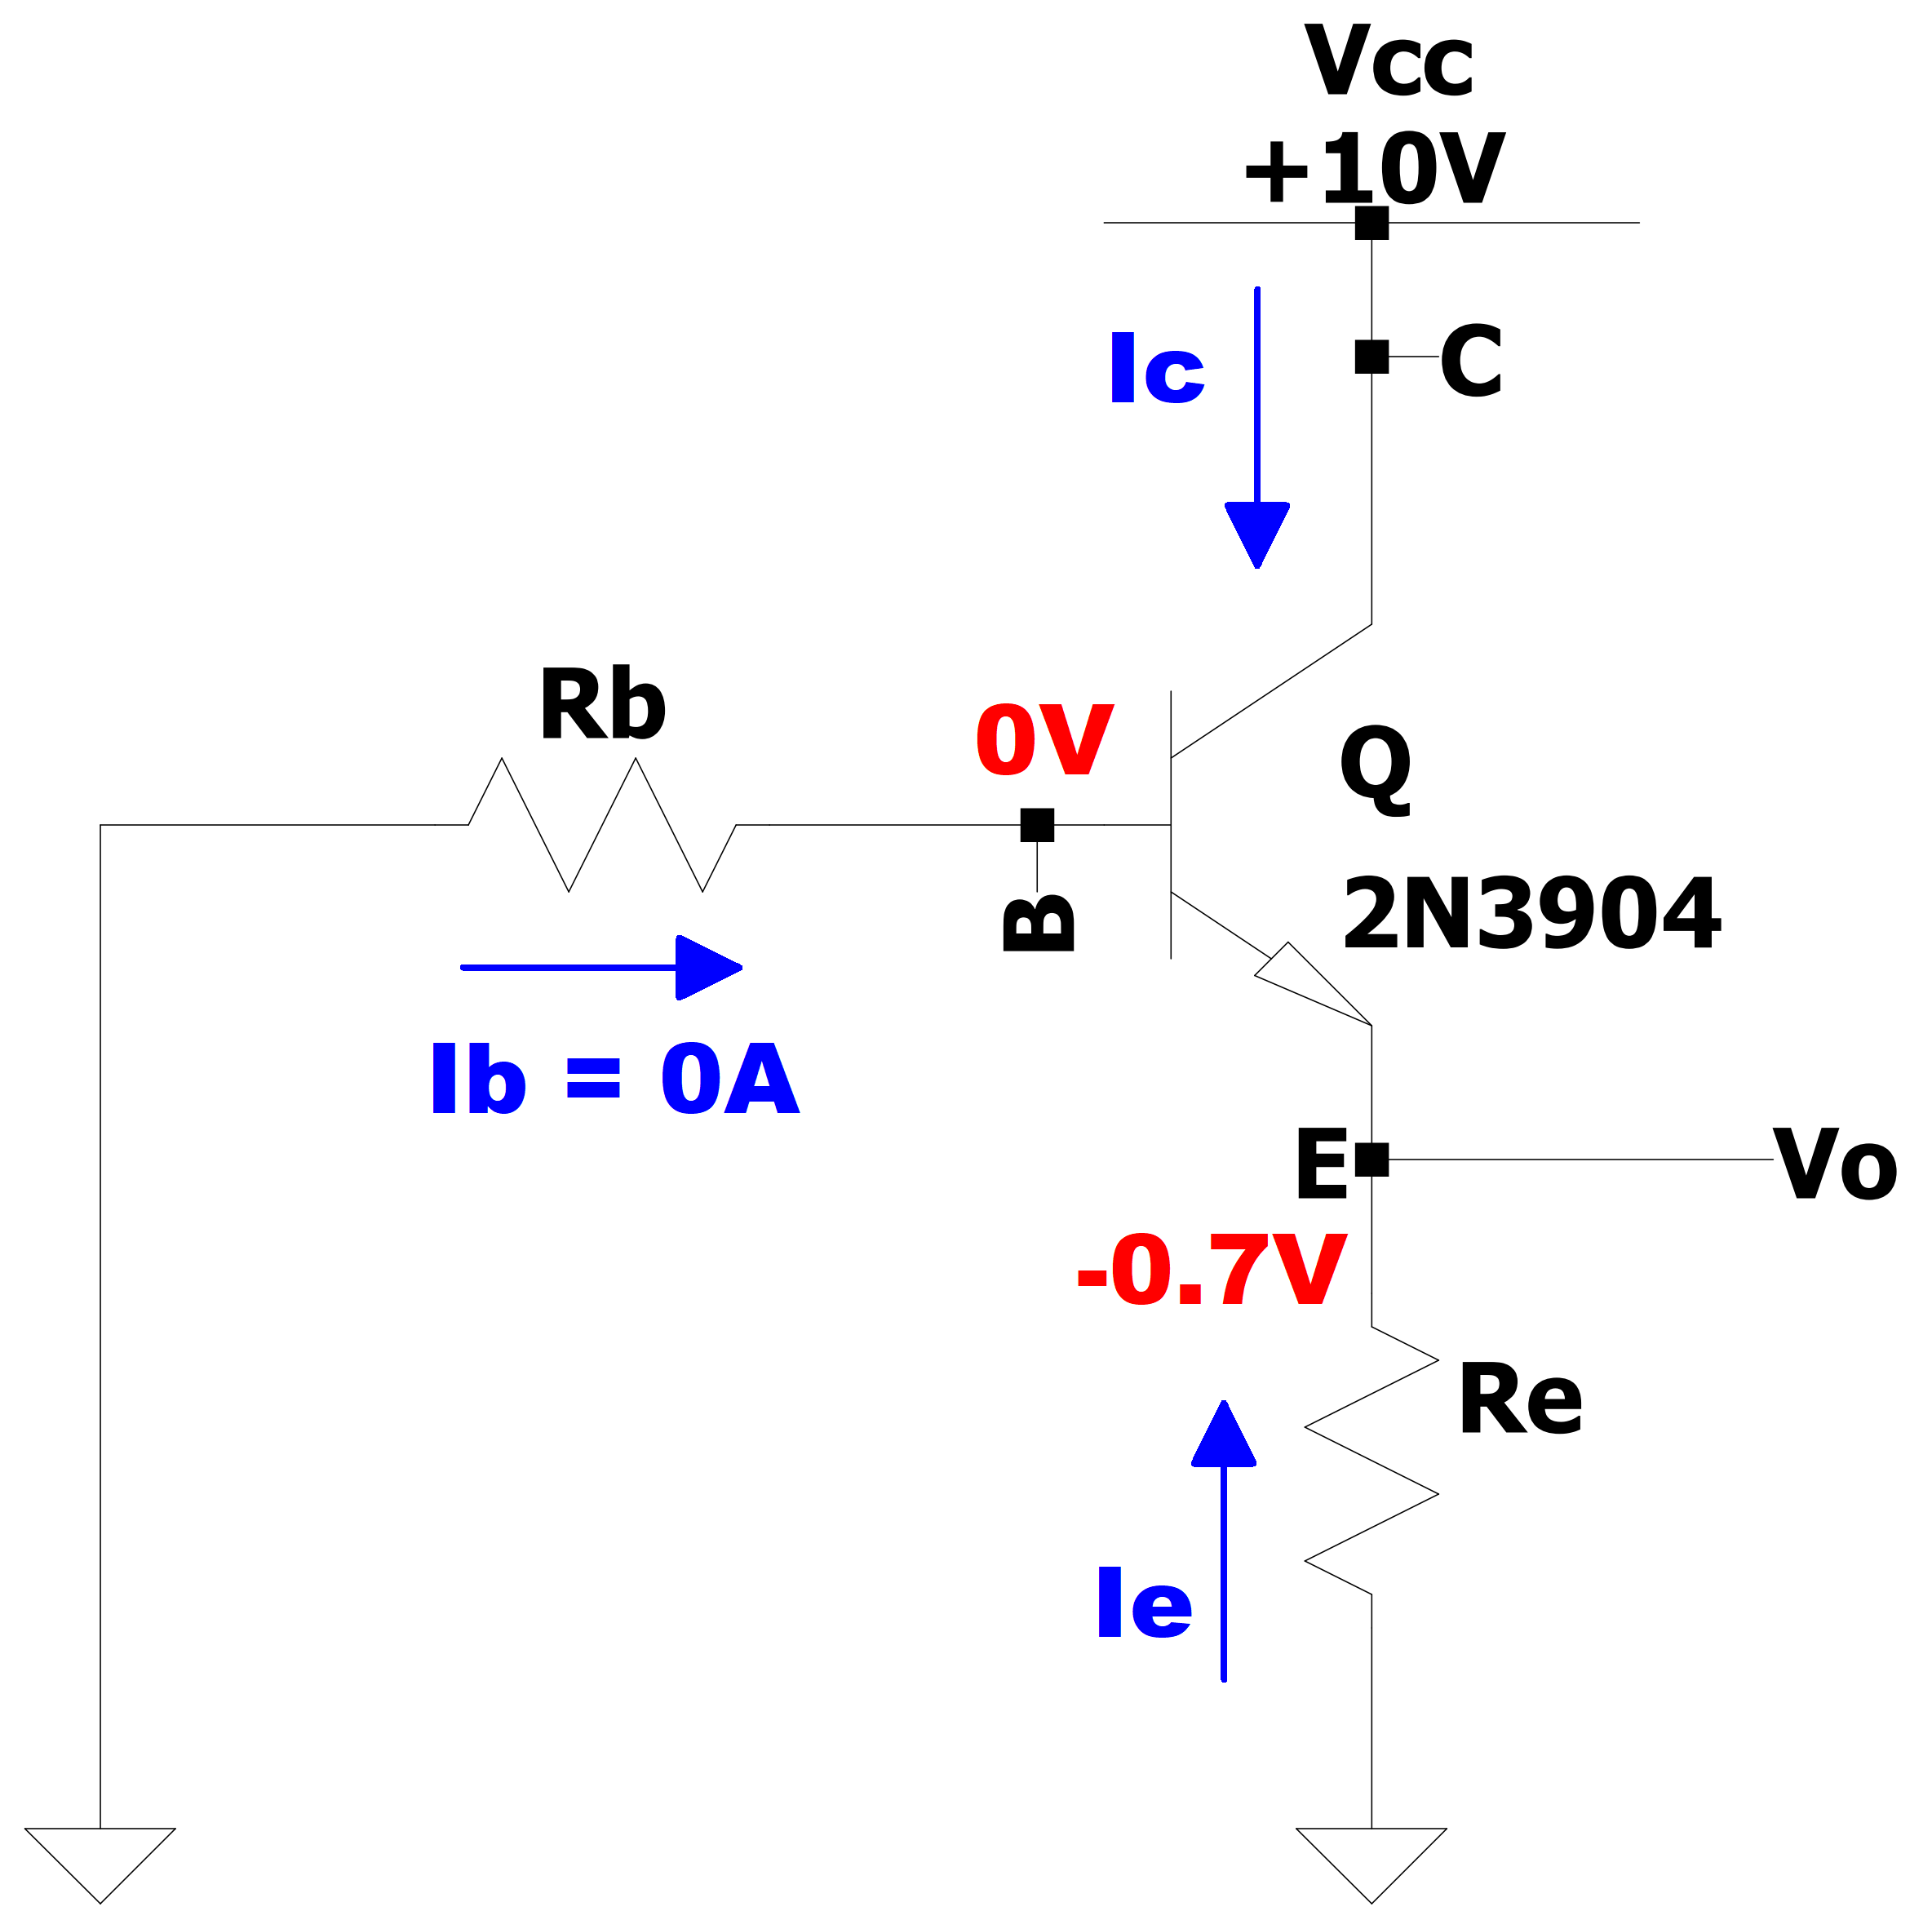
\includegraphics[height=9cm]{immagini/EFv2_1_pl}
\caption{Punto di lavoro dell'\textit{Emitter follower} ad alimentazione singola.}
\label{figura:EFv2_1_pl}
\end{figure}
\\Utilizziamo ancora il modello ideale del transistor, perciò assumiamo che $\displaystyle{\beta\rightarrow\infty}$ e che $I_{B}=0A$. Allora, la corrente che fluisce nella resistenza  $R_B$ è nulla, quindi sarà nulla anche la caduta di tensione ai suoi capi, di conseguenza $V_B=0V$.
\\\indent Suppondendo che il transistor si trovi in regione attiva diretta, la tensione $V_{BE}$ fra la base e l'emettitore è pari a circa +0.7V perché la giunzione è polarizzata direttamente. Dato che sappiamo che $V_{B}=0V$, $V_{E}$ sarà uguale a -0.7V. 
\\\indent La resistenza $R_E$ è attraversata da una corrente che va dalla massa all'emettitore: questo non è possibile, perché implicherebbe che la corrente entri nel transistor e fluisca dall'emettitore al collettore, ovvero nel verso opposto rispetto a quello consentito. Questo porta ad affermare che il transistor non può trovarsi in regione attiva diretta, ma è spento. Finché l'emettitore si trova ad una tensione minore di 0V, ovvero fin quando $V_B$ è minore di 0.7V, il circuito non funzionerà correttamente.
\\\indent Per ovviare a questo problema, bisogna fare in modo che la base del transistor si trovi ad una tensione adeguata. Per alzare il valore di tensione di questo nodo, possiamo sfruttare un partitore di resistenze. Inseriamo allora una resistenza da \SI{130}{k\ohm} fra la tensione di alimentazione e la base del transistor ed un'altra resistenza da \SI{150}{k\ohm} fra la base del transistor e massa. La resistenza di emettitore $R_E$ è invece pari a \SI{7.5}{k\ohm}. Il circuito è mostrato in figura \ref{figura:EFv2_2}.
\begin{figure}[h]
\centering
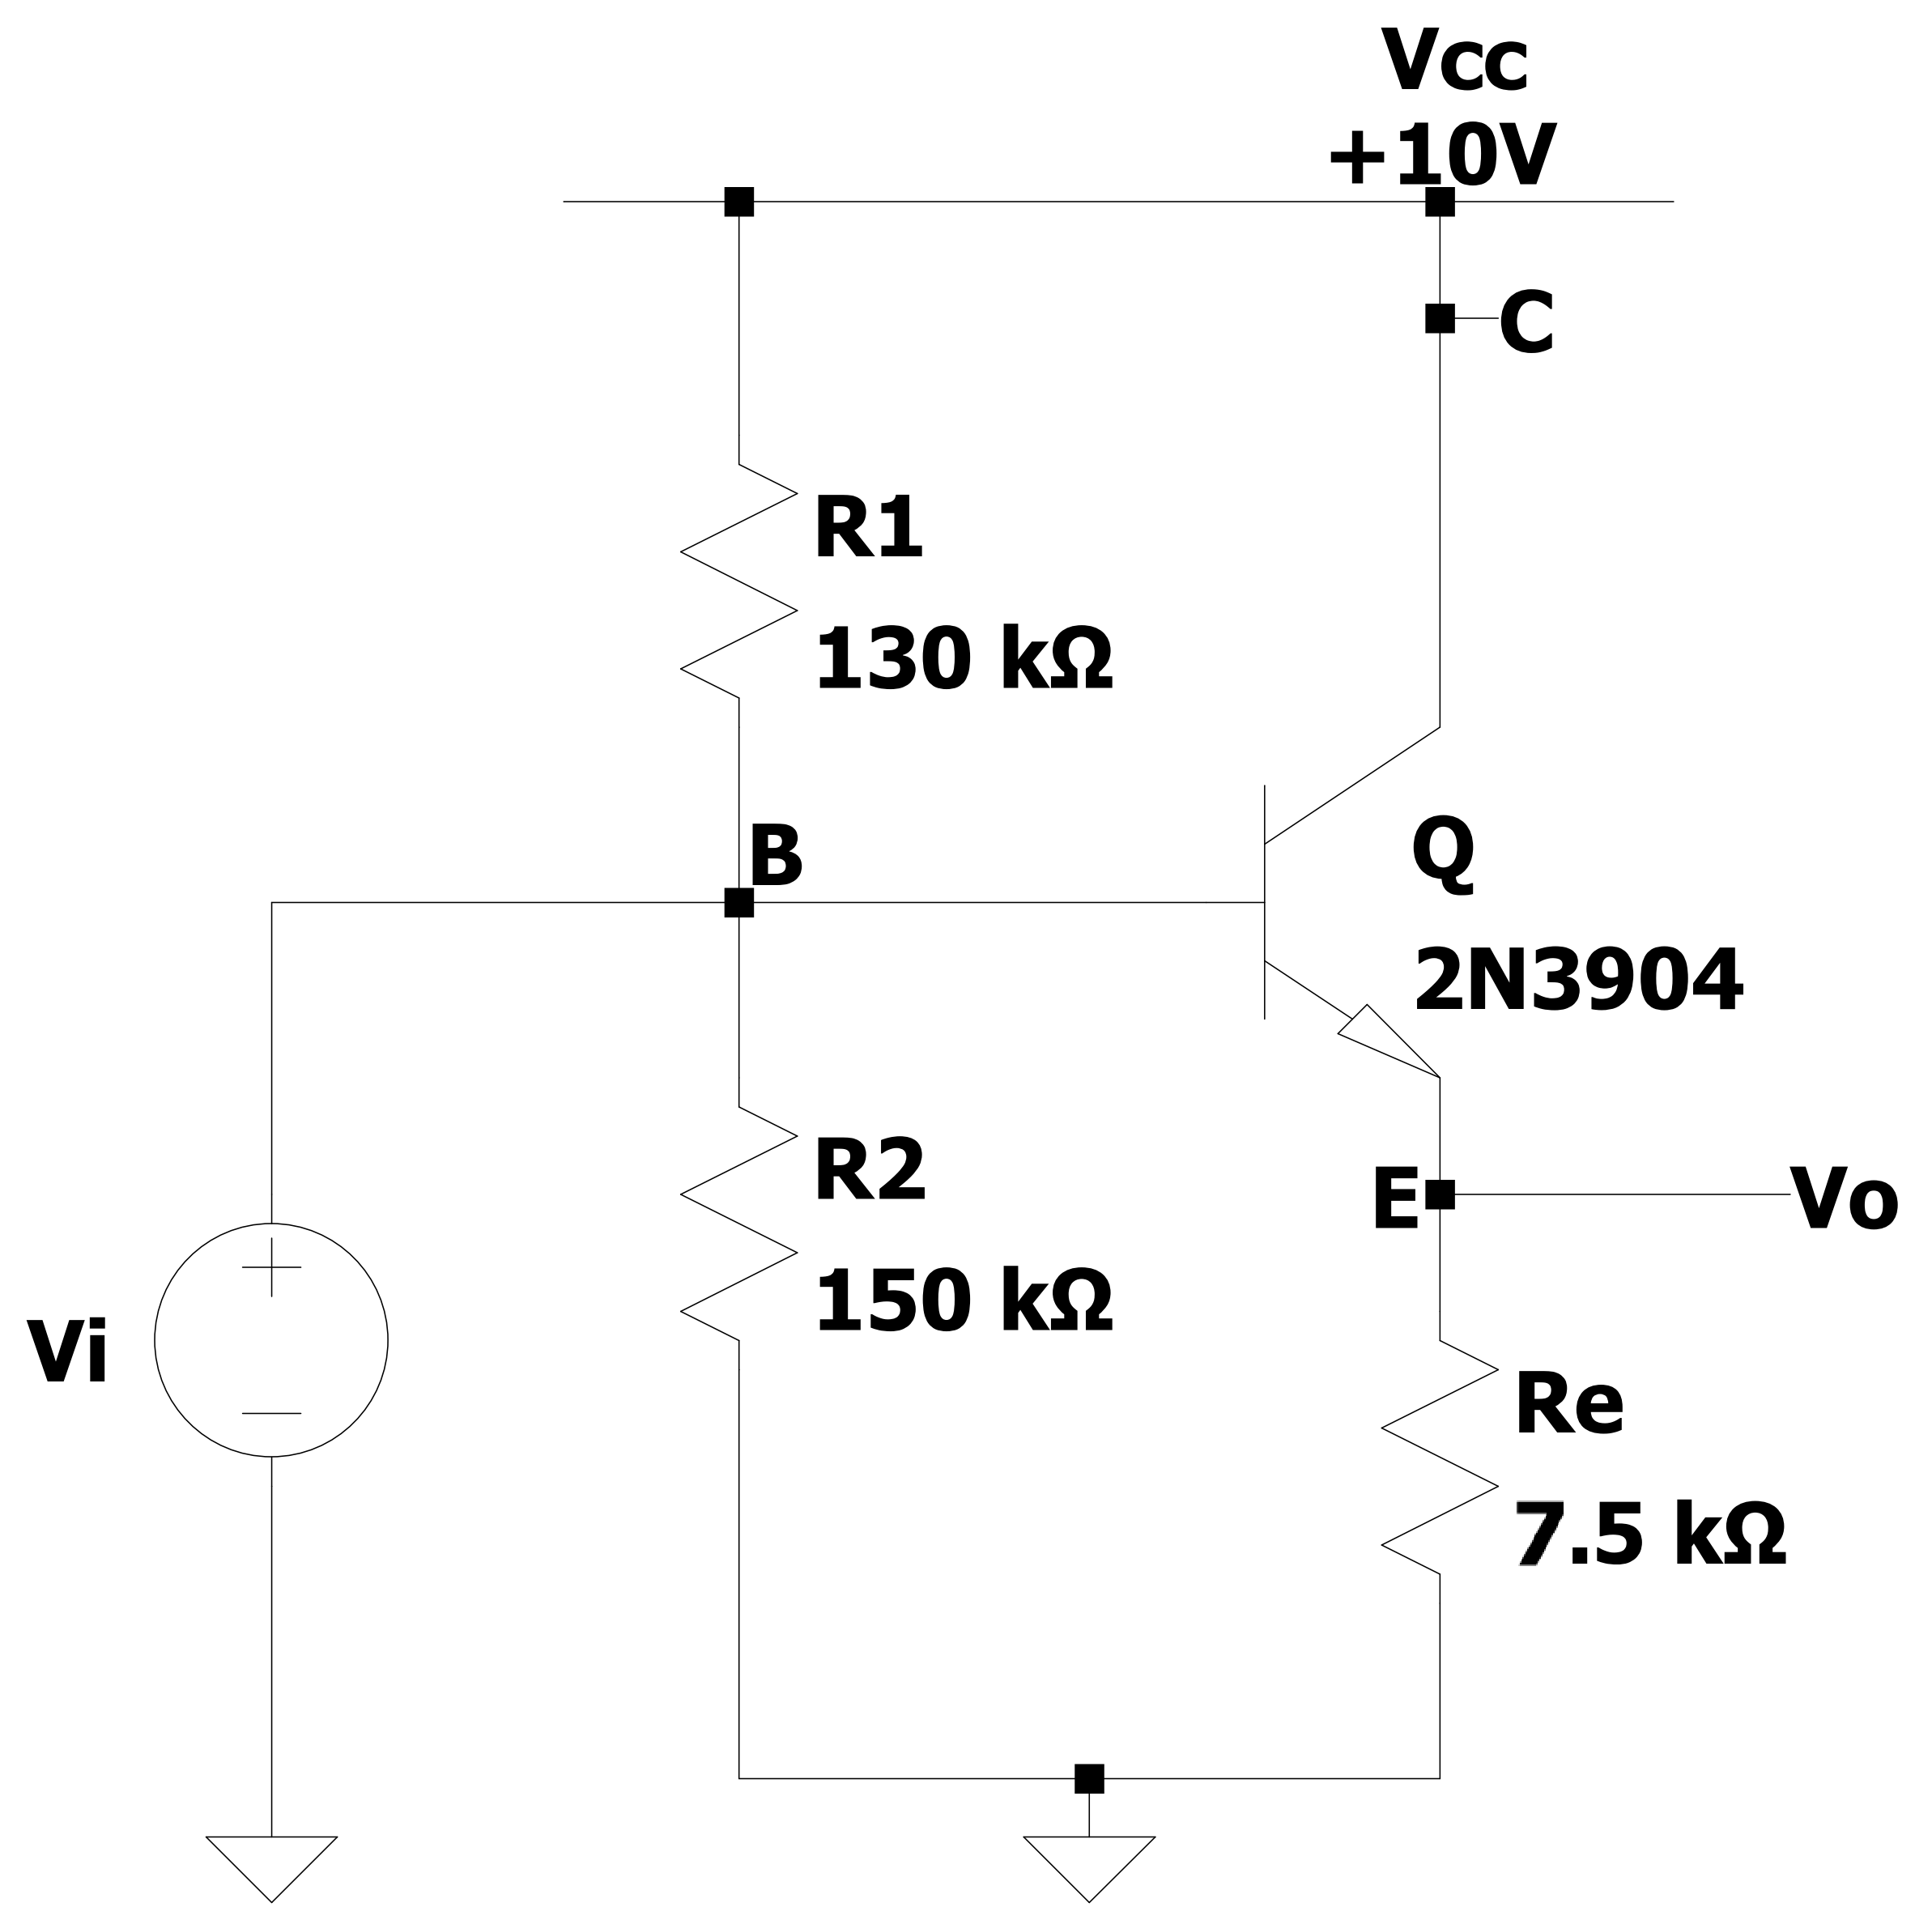
\includegraphics[height=9cm]{immagini/EFv2_2}
\caption{Schema modificato dell'\textit{Emitter follower} ad alimentazione singola.}
\label{figura:EFv2_2}
\end{figure}
\\\indent Ci accorgiamo subito che anche in questo caso il circuito non funziona come dovrebbe, perché sostituendo a $v_i$ un cortocircuito, forziamo ancora la base a massa. Bisogna fare in modo che il generatore di segnale sia disaccoppiato dal circuito in continua, così da evitare che la base venga forzata a massa, ma sia accoppiato in alternata, in modo tale che il segnale applicato in ingresso non venga modificato. Un componente che ha esattamente questo comportamento è il condensatore. \\Proviamo quindi a mettere un condensatore tra il segnale e la base del transistor. Il circuito risultante è la figura \ref{figura:EFv2_3}.
\begin{figure}[h!]
\centering
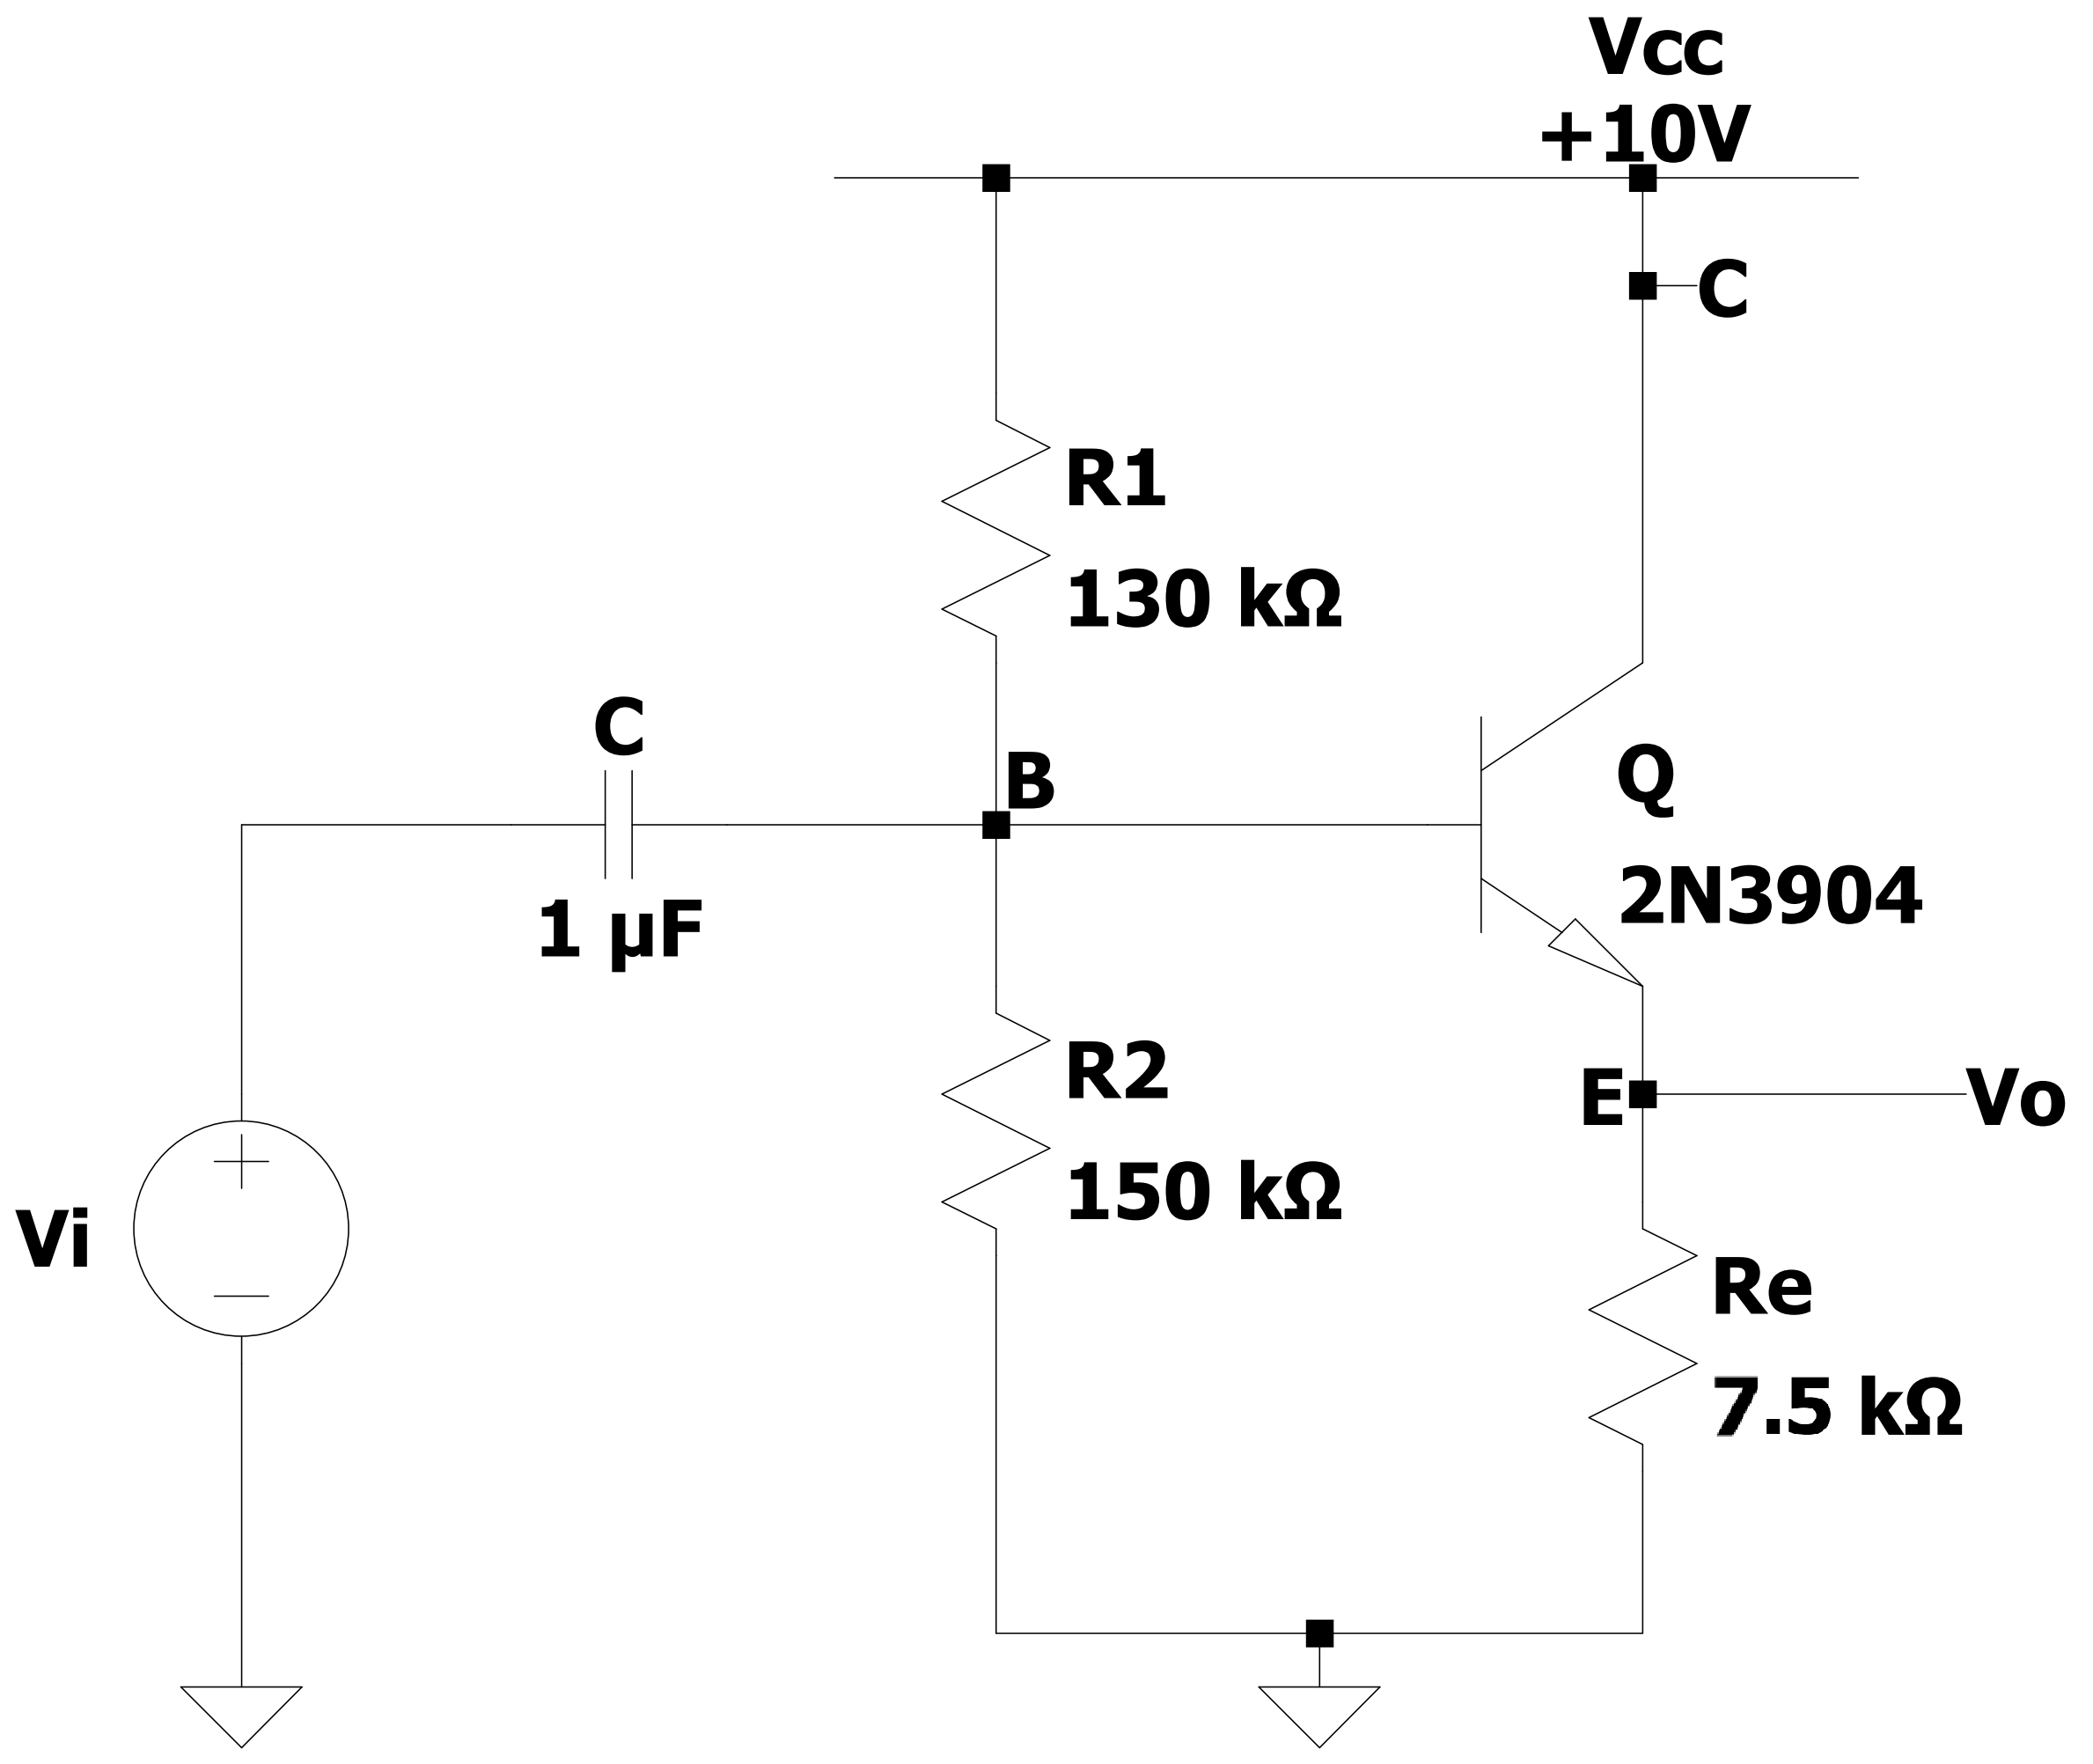
\includegraphics[height=9cm]{immagini/EFv2_3}
\caption{Schema finale dell'\textit{Emitter follower} ad alimentazione singola.}
\label{figura:EFv2_3}
\end{figure}
\\\indent Ora possiamo proseguire l'analisi. Per il punto di lavoro sostituiamo il generatore di segnale con un cortocircuito e il condensatore con un circuito aperto, perciò c'è un circuito aperto fra la massa e la base del transistor, proprio come ci aspettavamo. Lo schema è riportato in figura \ref{figura:EFv2_3_pl}.
\begin{figure}[h]
\centering
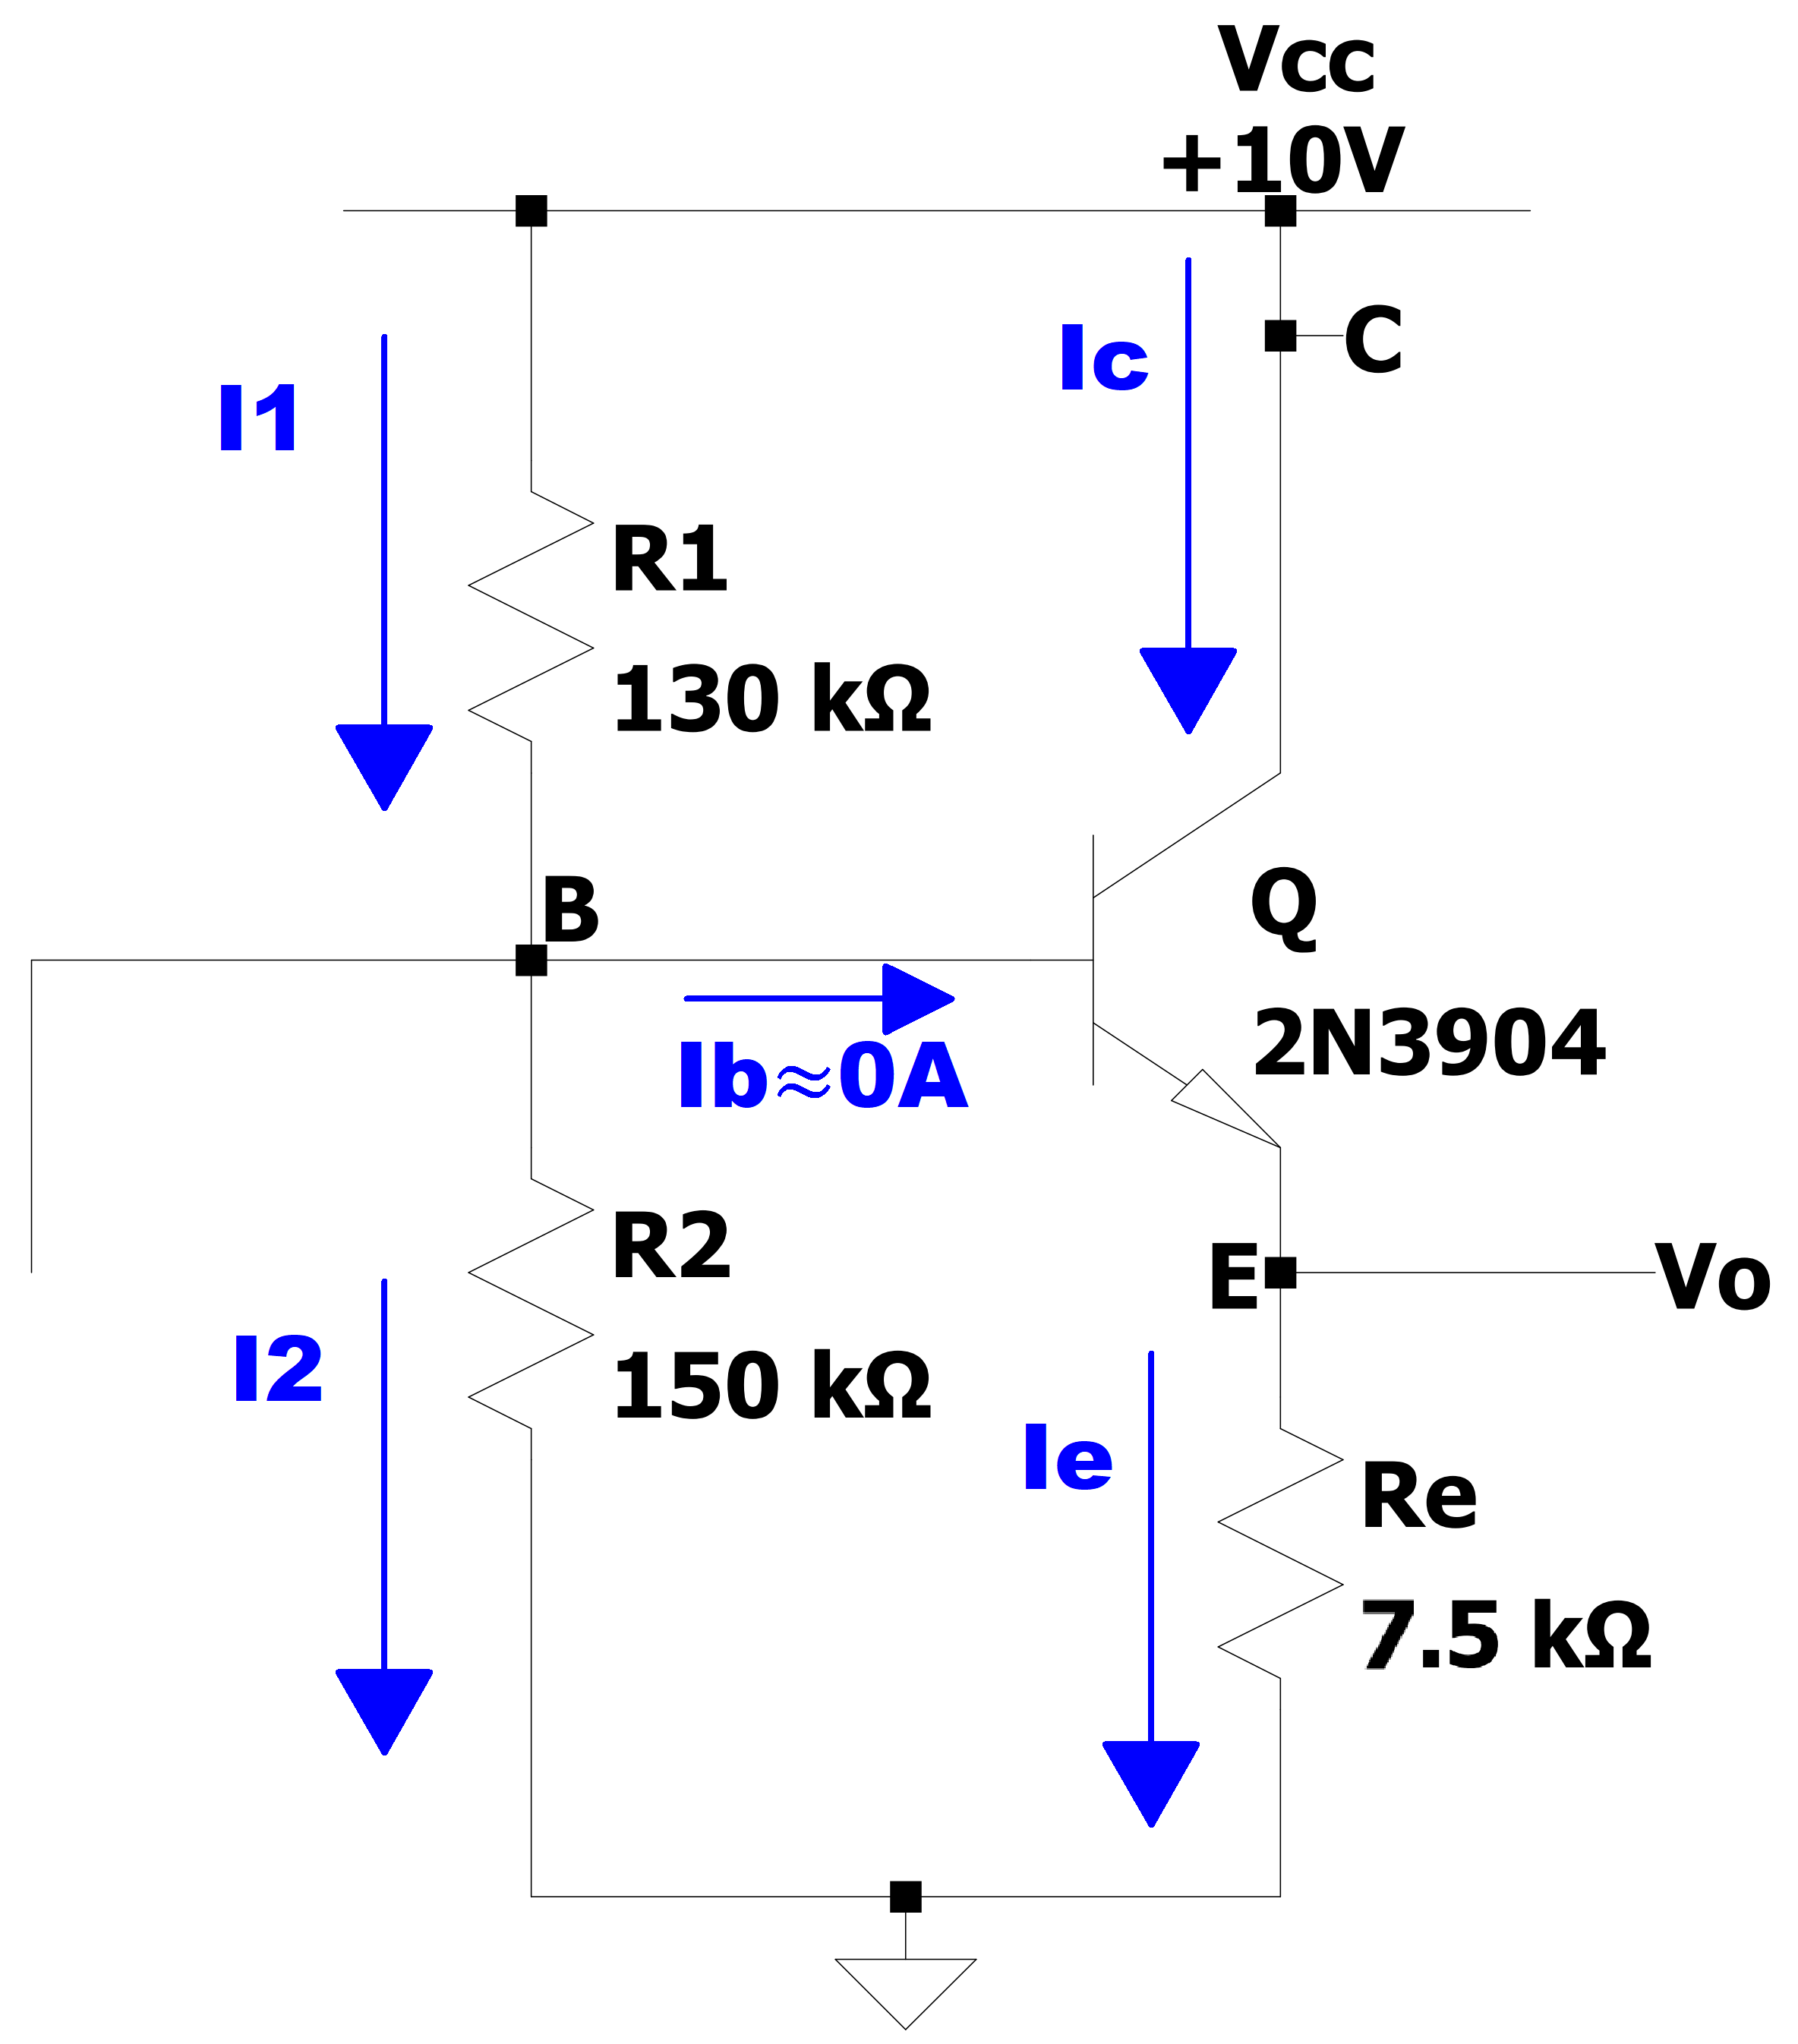
\includegraphics[height=10cm]{immagini/EFv2_3_pl}
\caption{Schema finale del punto di lavoro dell'\textit{Emitter follower} ad alimentazione singola.}
\label{figura:EFv2_3_pl}
\end{figure}
\\Risolviamo il circuito, sempre nell'ipotesi che $\displaystyle{\beta\rightarrow\infty}$ e che quindi $I_{B}=0A$. La tensione $V_B$ può essere ricavata applicando Kirchhoff alla base del transistor, oppure, più semplicemente, si può usare la formula del partitore di tensione:
\\[2pt]\indent$\displaystyle{V_B=\frac{R_2}{R_1+R_2}\cdot 10V=\frac{\SI{150}{k\ohm}}{\SI{280}{k\ohm}}\cdot 10V=5.357V}$
\\[2pt]Dato che $I_B$ è nulla, applicando la legge di Kirchhoff al nodo B otteniamo che $I_1=I_2$, possiamo ricavare una delle due correnti con la legge di Ohm, per esempio calcoliamo $I_2$:
\\[2pt]\indent$\displaystyle{I_2=\frac{V_B-0V}{R_2}=\frac{5.357V}{\SI{150}{k\ohm}}=0.0357mA}$
\\[2pt]Si noti che avremmo ottenuto lo stesso valore se avessimo calcolato $I_1$ al posto che $I_2$.
\\Per calcolare le tensioni e le correnti mancanti si procede esattamente come è stato fatto per l'\textit{Emitter follower} ad alimentazione duale, nella sezione \ref{puntolavoroEFv1}. Bisogna fare attenzione che cambiano i valori delle tensioni e la resistenza $R_E$, perciò saranno diverse anche le correnti che scorrono nei vari rami. 
\\Nella tabella \ref{table:EFv2_3_pl} sono riassunte tutte le grandezze ricavate dal punto di lavoro di questo circuito. 
\begin{table}[h]
	\centering
	\begin{tabular}{|c|c|c|c|c|c|c|c|c|}
		\hline
		\textbf{V\ped{B}[V]} & \textbf{V\ped{C}[V]} & \textbf{V\ped{E}[V]} & \textbf{I\ped{B}[A]} & \textbf{I\ped{1}[mA]} & \textbf{I\ped{2}[mA]} & \textbf{I\ped{E}[mA]} & \textbf{I\ped{C}[mA]} & \textbf{g\ped{m}[A/V]} \\ 
		\hline
		5.357 & 10 & 4.657 & 0 & 0.0357 & 0.0357 & 0.6209 & 0.6209 & 0.024\\ 
		\hline
	\end{tabular}
\caption{Riassunto delle grandezze ricavate dal punto di lavoro del circuito appena discusso.}
\label{table:EFv2_3_pl}
\end{table}
\subsection{Analisi di piccolo segnale}  
Per l'analisi di piccolo segnale consideriamo lo schema di figura \ref{figura:EFv2_3}. Sostituiamo l'alimentazione positiva a 10V con la massa, al posto del transistor utilizziamo il suo modello per piccolo segnale a bassa frequenza ed il condensatore, per ora, non lo sostituiamo con un cortocircuito. Lo schema diventa pertanto quello mostrato in figura \ref{figura:EFv2_3_ps}.
\begin{figure}[h]
\centering
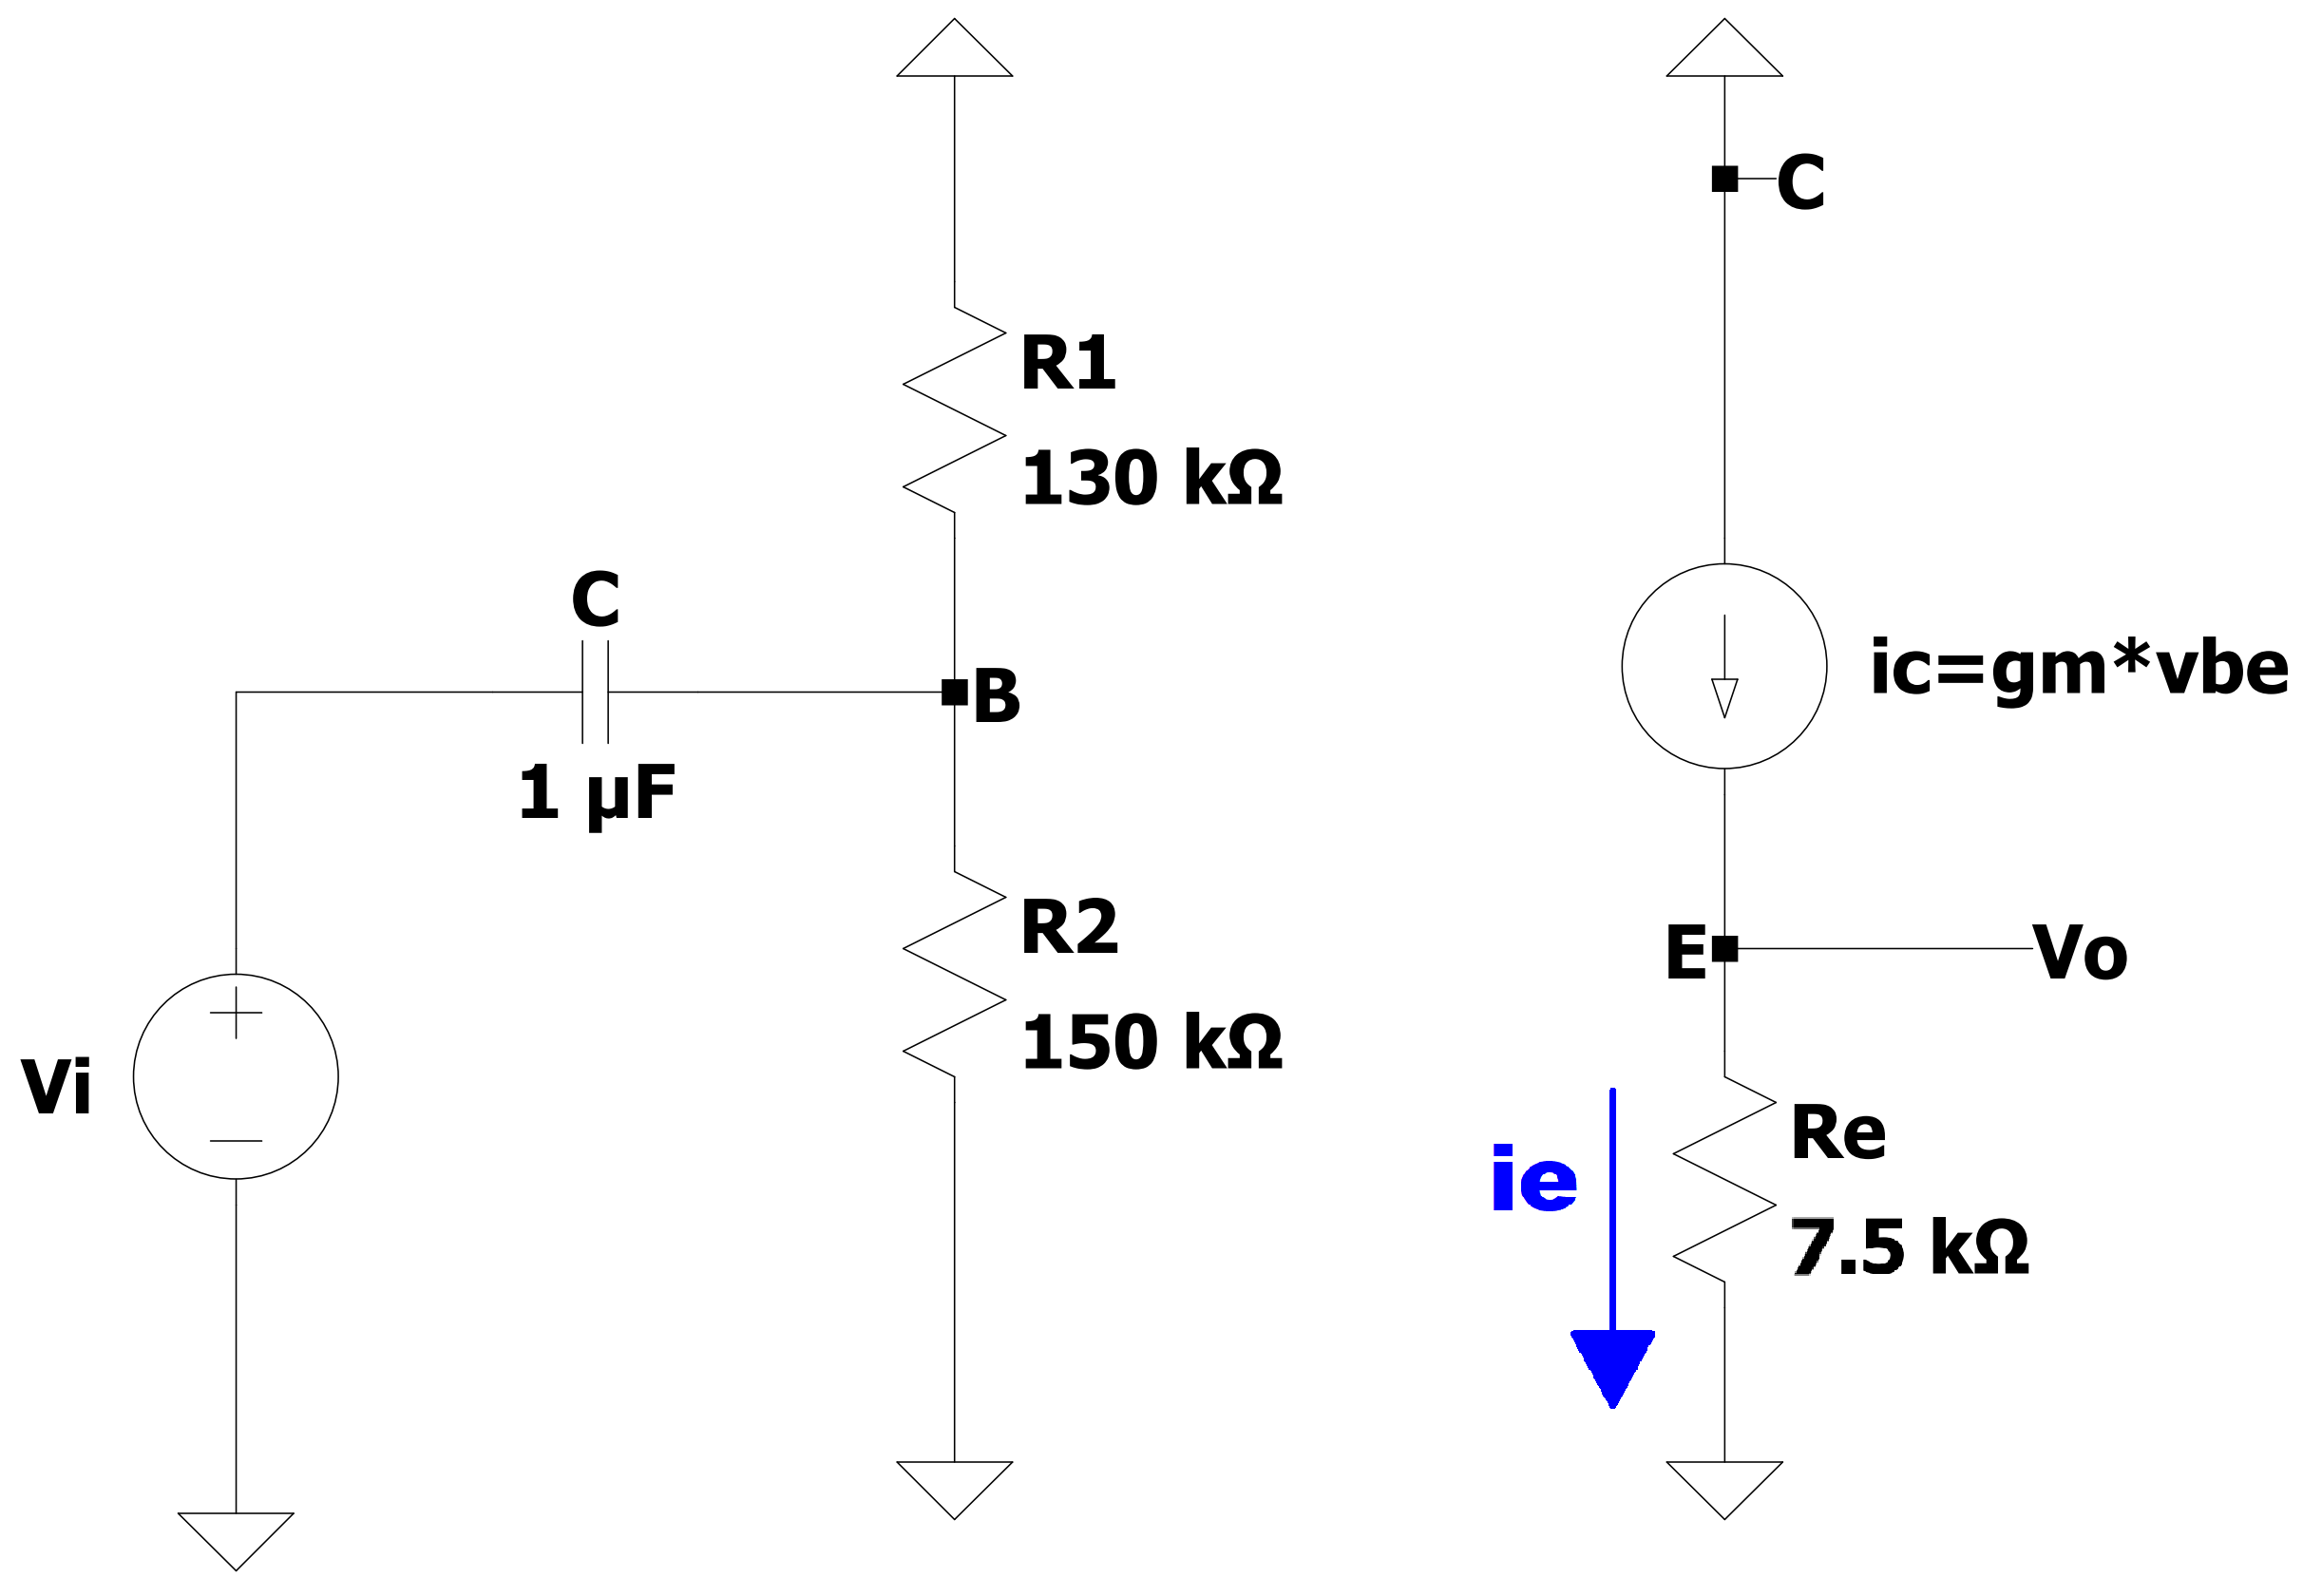
\includegraphics[height=10cm]{immagini/EFv2_3_ps}
\caption{Schema finale dell'analisi di piccolo segnale dell'\textit{Emitter follower} ad alimentazione singola.}
\label{figura:EFv2_3_ps}
\end{figure}
\\Il circuito di destra è identico a quello dell'\textit{Emitter follower} ad alimentazione di duale, cambia solo il valore della resistenza $R_E$. Nel circuito di sinistra possiamo invece riconoscere un filtro passa-alto formato dal condensatore $C$ e dal parallelo fra le resistenze $R_1$ e $R_2$. La frequenza di taglio di questo filtro è:
\\[2pt]\indent $\displaystyle{f_T=\frac{1}{2\pi\cdot C\cdot (R_1\parallelsum R_2)}=\frac{1}{2\pi\cdot 1\mu F\cdot(\SI{130}{k\ohm}\parallelsum\SI{150}{k\ohm})}=\SI{2.285}{\hertz}}$
\\[2pt]Se la frequenza di taglio è sufficientemente bassa, come nel nostro caso, il contributo del filtro passa-alto alla funzione di trasferimento del circuito è trascurabile, pertanto $v_o=v_i$. In caso contrario, nella funzione di trasferimento finale bisogna considerare anche la funzione di trasferimento del filtro.
\subsection{Componenti, strumenti e misure} 
Prima di realizzare la versione finale del circuito \textit{Emitter follower} ad alimentazione singola, abbiamo provato a collegare a massa l'alimentazione negativa del circuito utilizzato prima. In figura \ref{figura:oscillo2} sono riportate la tensione in ingresso e la tensione in uscita al circuito appena modificato. I due segnali sono stati accoppiati in DC.
\begin{figure}[h]
\centering
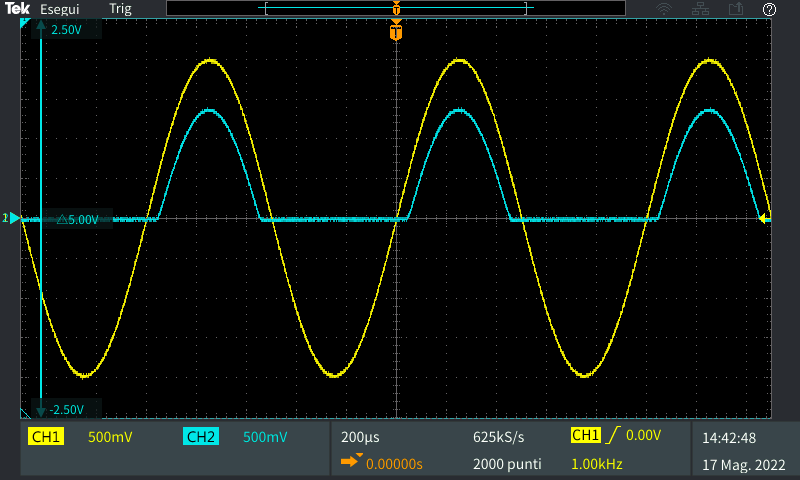
\includegraphics[height=7cm]{immagini/oscillo2}
\caption{Grafico della tensione in ingresso (CH1) e della tensione in uscita (CH2) al circuito.}
\label{figura:oscillo2}
\end{figure}
\\\indent Come ci aspettavamo, il circuito taglia le semionde negative: quando il segnale in ingresso è minore di 0.7V, la tensione in uscita rimane a 0V. Dal grafico possiamo anche vedere che la caduta di tensione data dalla giunzione p-n fra base ed emettitore rimane.
\\\indent Dopo aver verificato che il circuito si comporta come ci aspettavamo dall'analisi teorica, abbiamo costruito la versione finale già illustrata in figura \ref{figura:EFv2_3}. Il circuito, di cui si riporta la fotografia (figura \ref{figura:fotoEFv2_3}), è stato realizzato su una breadboard utilizzando questi componenti:
\begin{itemize}
\item transistor bipolare NPN 2N3904;
\item due resistenze connesse in serie, $R_{E_1}$ e $R_{E_2}$, entrambe da \SI{3.9}{k\ohm}, per realizzare la resistenza $R_E$ da \SI{7.8}{k\ohm};
%% da QUI
\item due resistenze, una da \SI{82}{k\ohm} ($R_{11}$) ed una da \SI{39}{k\ohm} ($R_{12}$) connesse in serie, per realizzare la resistenza $R_1$ da \SI{120}{k\ohm};
\item tre resistenze, una da \SI{39}{k\ohm} ($R_{21}$), una da \SI{27}{k\ohm} ($R_{22}$) ed una da \SI{82}{k\ohm} ($R_{23}$) connesse in serie, per realizzare la resistenza $R_2$ da \SI{148}{k\ohm};
\item un condensatore da \SI{1}{\mu\farad}.
\end{itemize}
Per quanto riguarda $R_E$, non è stato possibile utilizzare una resistenza del valore indicato (\SI{7.5}{k\ohm}), ma con queste connessioni otteniamo una resistenza di valore poco maggiore (solo il 4\%). Lo stesso discorso vale per le altre due resistenze, però quello che conta in questo caso non è tanto il valore del singolo componente, quanto il fattore di partizione. Il fattore di partizione che dovremmo ottenere è di 0.5357, quello che otteniamo è di 0.5522, ovvero solo il 3\% in più.
\begin{figure}[h]
\centering
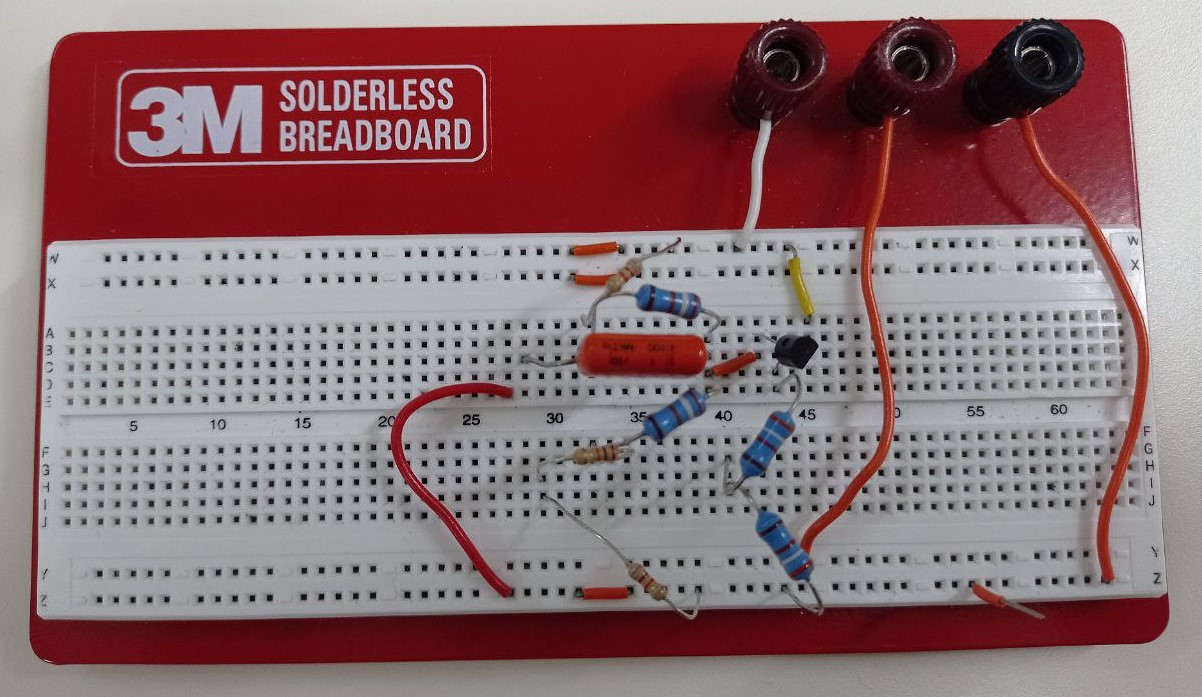
\includegraphics[height=8.5cm]{immagini/fotoEFv2_3}
\caption{Fotografia del circuito \textit{Emitter follower} ad alimentazione singola realizzato in laboratorio.}
\label{figura:fotoEFv2_3}
\end{figure}
\\Per le misure e le analisi, sono stati utilizzati i seguenti strumenti:
\begin{itemize}
\item alimentatore da banco, con alimentazione positiva impostata a 10V e limite in corrente di 50mA;
\item generatore di forme d'onda;
\item multimetro da banco;
\item oscilloscopio a due canali.
\end{itemize}
Come per il circuito precedente, per prima cosa andiamo a misurare il valore delle resistenze con il multimetro ed i valori delle tensioni delle giunzioni p-n del transistor. I valori ottenuti sono mostrati in tabella \ref{table:EFv2_3_comp}.
\\
\begin{table}[h]
	\centering
	\begin{tabular}{|c|c|c|}
	\cline{2-3} 
	\multicolumn{1}{c|}{} & \textbf{Valore nominale} & \textbf{Valore misurato}\\ 
		%\hline
		%{} & \textbf{Valore nominale} & \textbf{Valore misurato} \\ 
		\hline
		$\mathbf{R_{E_1}}$& \SI{3.9}{k\ohm} & \SI{3.88}{k\ohm} \\ 
		\hline
		$\mathbf{R_{E_2}}$& \SI{3.9}{k\ohm} & \SI{3.91}{k\ohm} \\ 
		\hline
		$\mathbf{R_{11}}$& \SI{82}{k\ohm} & \SI{82.67}{k\ohm} \\ 
		\hline
		$\mathbf{R_{12}}$& \SI{39}{k\ohm} & \SI{38.86}{k\ohm} \\ 
		\hline
		$\mathbf{R_{21}}$& \SI{39}{k\ohm} & \SI{38.80}{k\ohm} \\ 
		\hline
		$\mathbf{R_{22}}$& \SI{27}{k\ohm} & \SI{26.87}{k\ohm} \\ %CONTROLLA VALORE
		\hline
		$\mathbf{R_{23}}$& \SI{82}{k\ohm} & \SI{82.18}{k\ohm} \\ 
		\hline
		$\mathbf{V_{BE}}$& $\mathrm{ \simeq0.7V}$ & 0.699V \\ 
		\hline
		$\mathbf{V_{BC}}$& $\mathrm{ \simeq0.7V}$  & 0.659V \\ 
		\hline
	\end{tabular}
\caption{Grandezze misurate prima di realizzare il circuito.}
\label{table:EFv2_3_comp}
\end{table}
\\I valori delle resistenze saranno quindi $R_E=\SI{7.79}{k\ohm}$, $R_1=\SI{121.53}{k\ohm}$ e $R_2=\SI{147.85}{k\ohm}$. Ora studiamo il punto di lavoro del circuito. Misuriamo le tensioni dei nodi B ed E con il multimetro e calcoliamo le correnti $I_1$, $I_2$ e $I_E$ con la legge di Ohm. Ricaviamo quindi per differenza, applicando la legge di Kirchhoff, le correnti $I_B$ e $I_C$:
\\[2pt]\indent $\displaystyle{I_1=I_B+I_2\rightarrow I_B=I_1-I_2}$
\\\indent $\displaystyle{I_E=I_C+I_B\rightarrow I_C=I_E-I_B}$
\\[2pt]Tutti i valori misurati sono riportati in tabella \ref{table:EFv2_3_pl_mis}. Anche in questo caso le misure sono molto vicine ai valori teorici.
\begin{table}[h]
	\centering
	\begin{tabular}{|c|c|c|c|c|c|c|c|c|}
		\hline
		\textbf{V\ped{B}[V]} & \textbf{V\ped{C}[V]} & \textbf{V\ped{E}[V]} & \textbf{I\ped{1}[\textmu A]} & \textbf{I\ped{2}[\textmu A]} & \textbf{I\ped{E}[\textmu A]} & \textbf{I\ped{B}[\textmu A]} & \textbf{I\ped{C}[\textmu A]} & \textbf{g\ped{m}[A/V]} \\ 
		\hline
		5.228 & 10.000 & 4.607 & 39.27 & 35.36 & 591.40 & 3.91 & 587.49 & 0.023\\ 
		\hline
	\end{tabular}
\caption{Grandezze misurate dallo studio del punto di lavoro del circuito.}
\label{table:EFv2_3_pl_mis}
\end{table}
\\Terminato lo studio del punto di lavoro, applichiamo il segnale al circuito collegando il generatore di forme d'onda e osserviamo il grafico della tensione in ingresso e della tensione in uscita con l'oscilloscopio. La forma d'onda utilizzata è una sinusoide di frequenza $f=\SI{1}{k\hertz}$ e tensione picco-picco $V_{PP}$ di 2V. Il grafico è riportato in figura \ref{figura:oscillo3}, i due segnali sono accoppiati in DC.
\begin{figure}[h]
\centering
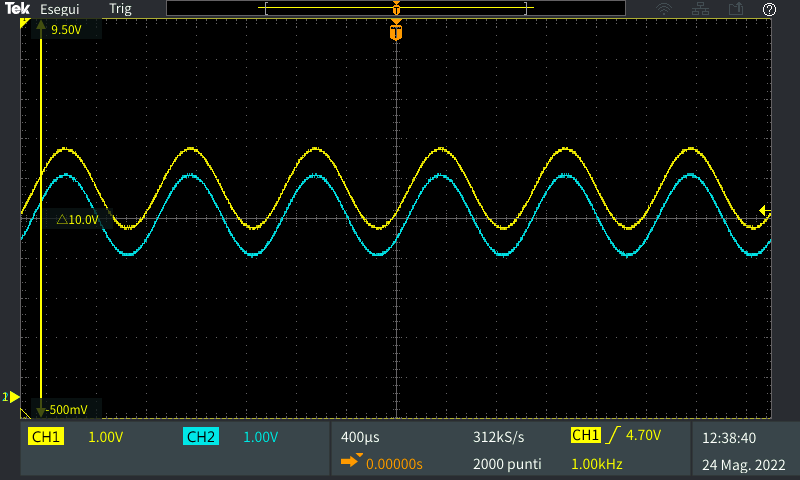
\includegraphics[height=7cm]{immagini/oscillo3}
\caption{Grafico della tensione in ingresso (CH1) e della tensione in uscita (CH2) al circuito.}
\label{figura:oscillo3}
\end{figure}
\\Dal grafico possiamo vedere che il guadagno del circuito è unitario perché entrambe le sinusoidi hanno la stessa ampiezza. La tensione applicata in ingresso, analogamente all'\textit{Emitter follower} ad alimentazione duale, la ritroviamo in uscita con una differenza di circa 0.7V, che è la caduta di tensione data dalla giunzione p-n fra base ed emettitore. I segnali di tensione in ingresso e in uscita sono in fase. 
\\Il grafico XY di un \textit{Emitter follower} è un tratto di retta con pendenza unitaria e quota -0.7, data dalla caduta di tenzione dell giunzione p-n fra base ed emettitore.
%----------------------------------------------------------------------------------------
%	CIRCUITO 2: COMMON EMITTER AMPLIFIER
%----------------------------------------------------------------------------------------
\clearpage
\newpage
\chapter{Circuito 2: Common Emitter Amplifier}
\section{Introduzione}
Vogliamo ora realizzare un circuito che funzioni come amplificatore. Se manteniamo l'emettitore ad una tensione costante e preleviamo l'uscita dal collettore, questo è possibile. Questo circuito è chiamato \textit{Common Emitter amplifier}. Abbiamo analizzato tre diverse versioni di questo circuito ma ne abbiamo realizzate solo due, una con alimentazione duale ed una con alimentazione singola, entrambe con la configurazione detta a \textit{degenerazione di emettitore}. 
\section{Prima versione} % senza degenerazione emitter, solo trattazione teorica non realizzato in lab
\label{CEv1_cap}
Questo schema è stato discusso solo dal punto di vista teorico. Di seguito si riportano lo schema e l'analisi del circuito. 
\subsection{Schema} 
Dato che faremo solo un'analisi teorica, trascuriamo sia il valore delle resistenze che il valore delle alimentazioni. Lo schema di riferimento è riportato in figura \ref{figura:CEv1}.
\begin{figure}[h]
\centering
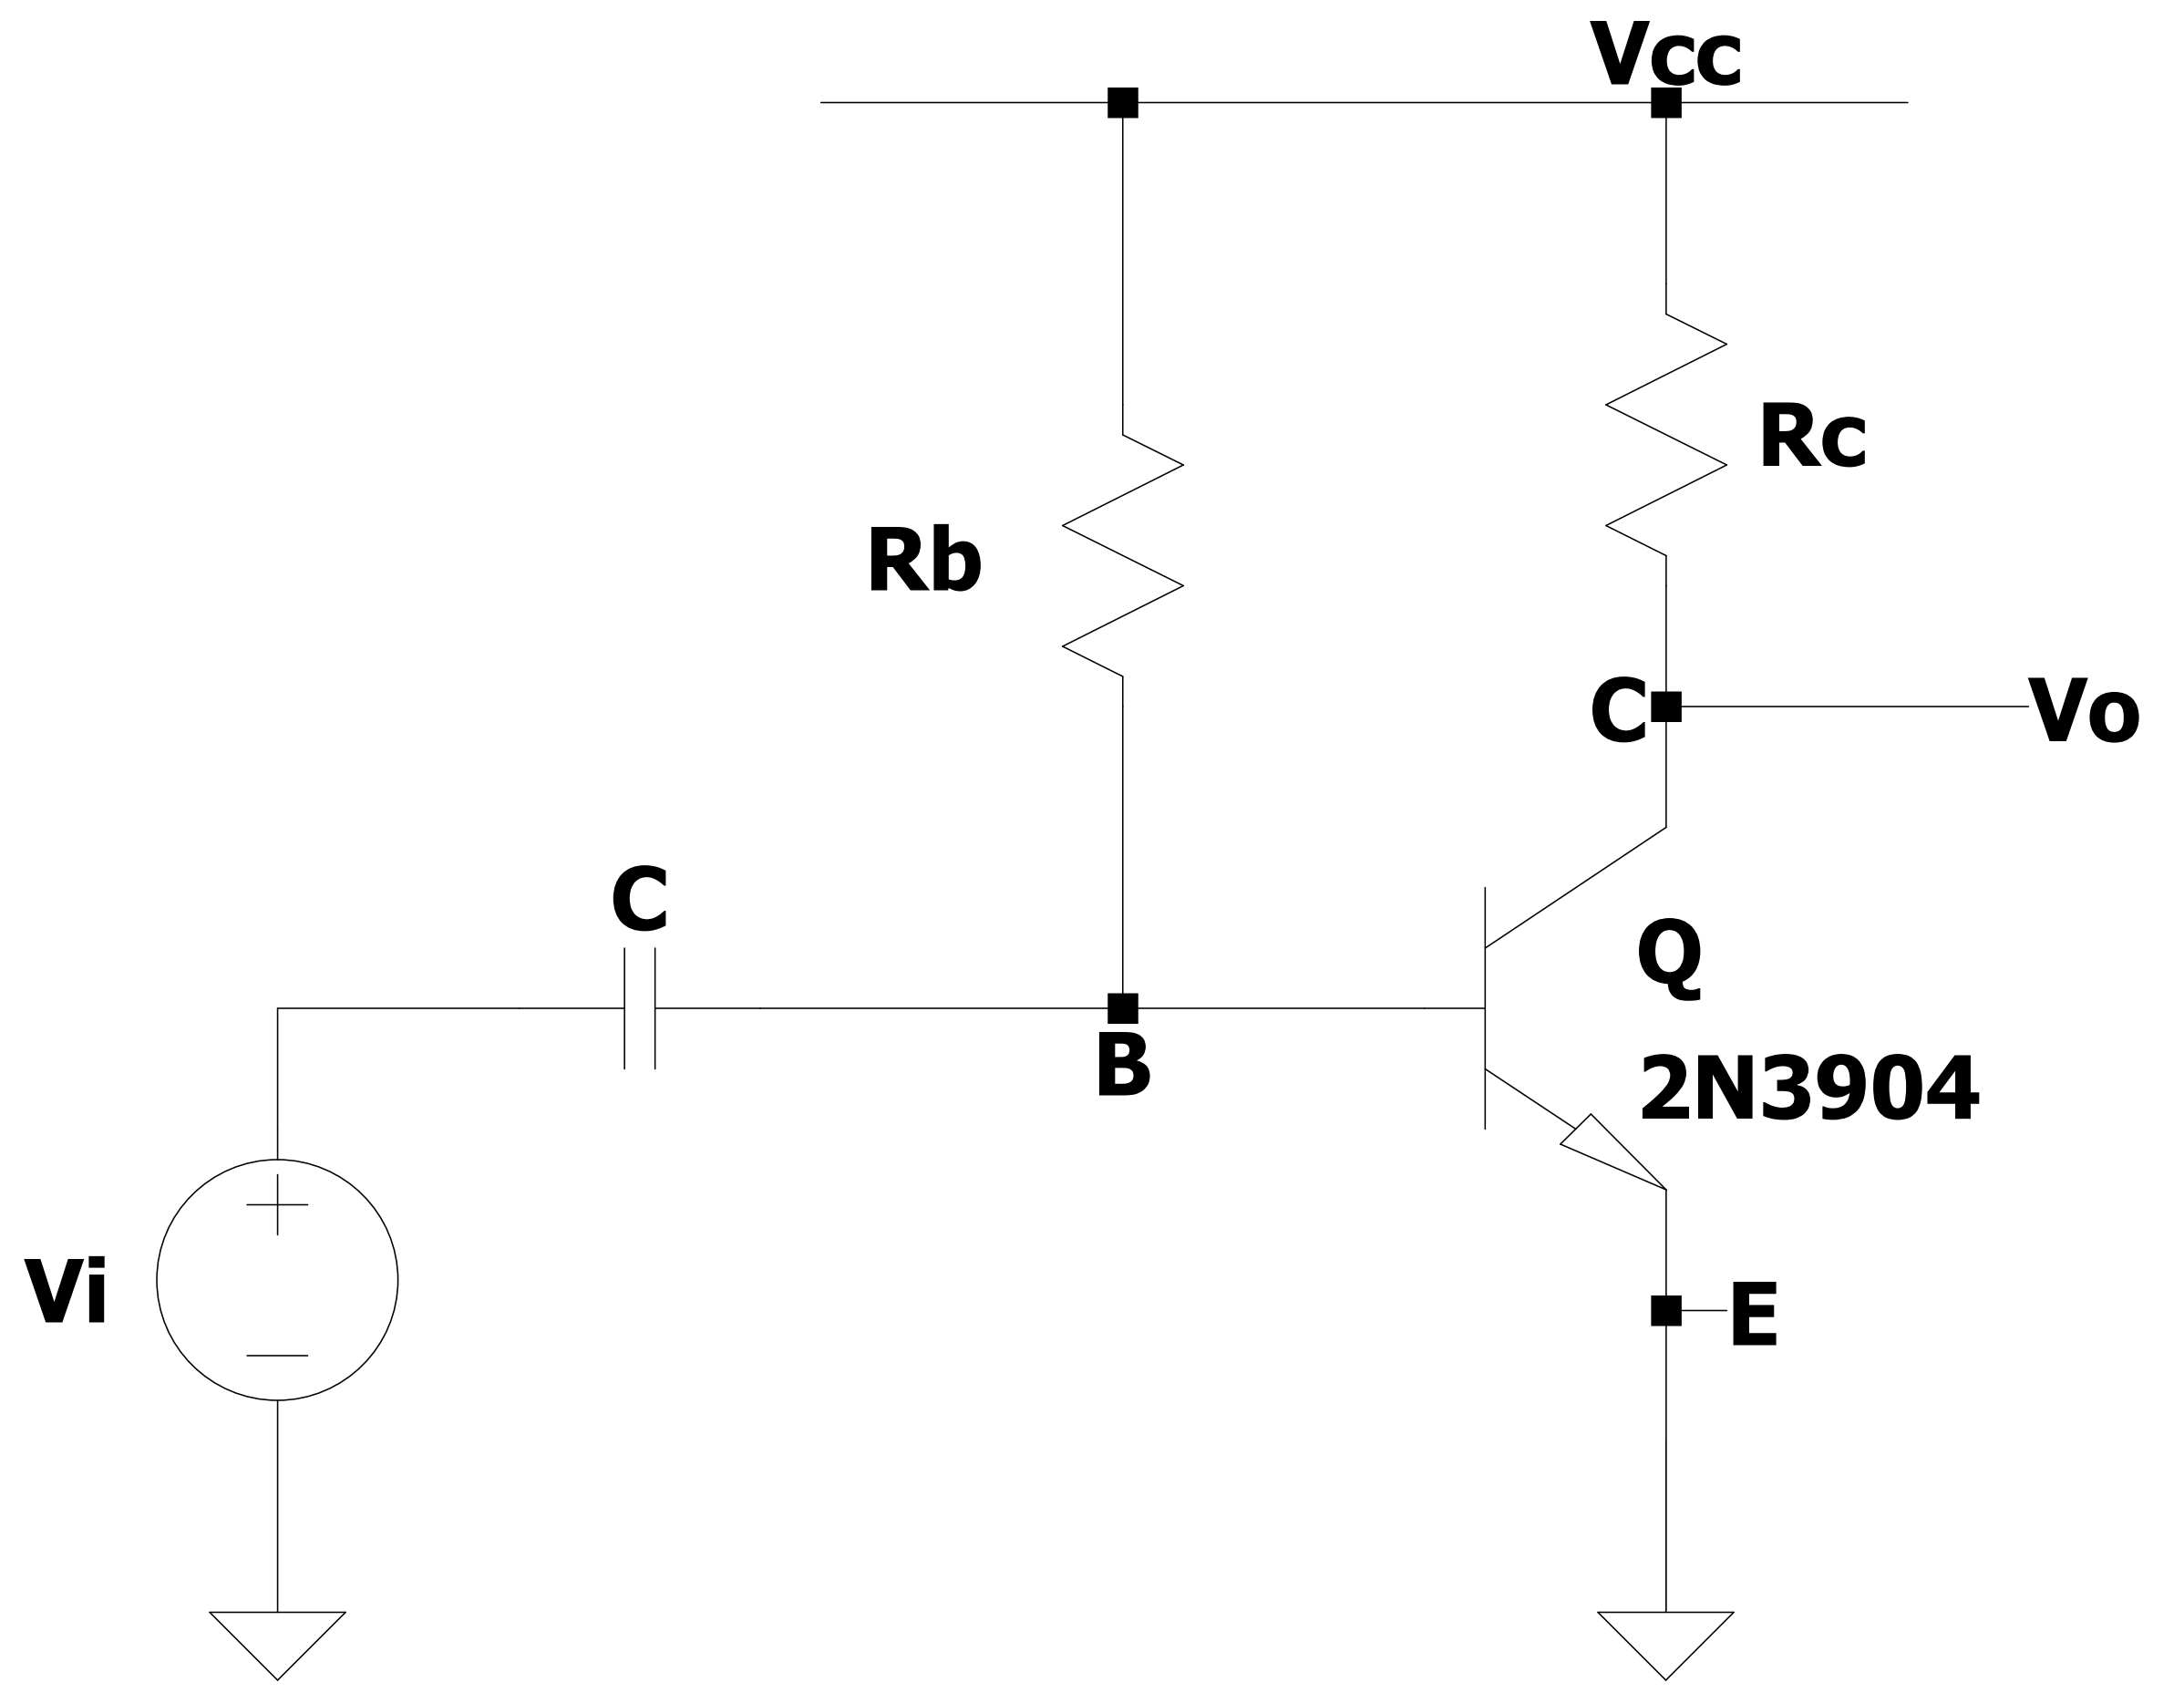
\includegraphics[height=7.9cm]{immagini/CEv1}
\caption{Schema del più semplice \textit{Common Emitter amplifier} realizzabile.}
\label{figura:CEv1}
\end{figure}
\subsection{Analisi del circuito} 
Consideriamo lo schema precedente. La determinazione del punto di lavoro non dà problemi. Passiamo allora all'analisi di piccolo segnale: per semplicità il condensatore diventa un cortocircuito, l'alimentazione $V_{CC}$ viene sostituita con la massa e al posto del transistor abbiamo il suo modello per piccolo segnale a bassa frequenza. Lo schema diventa quello mostrato in figura \ref{figura:CEv1_ps}.
\begin{figure}[h]
\centering
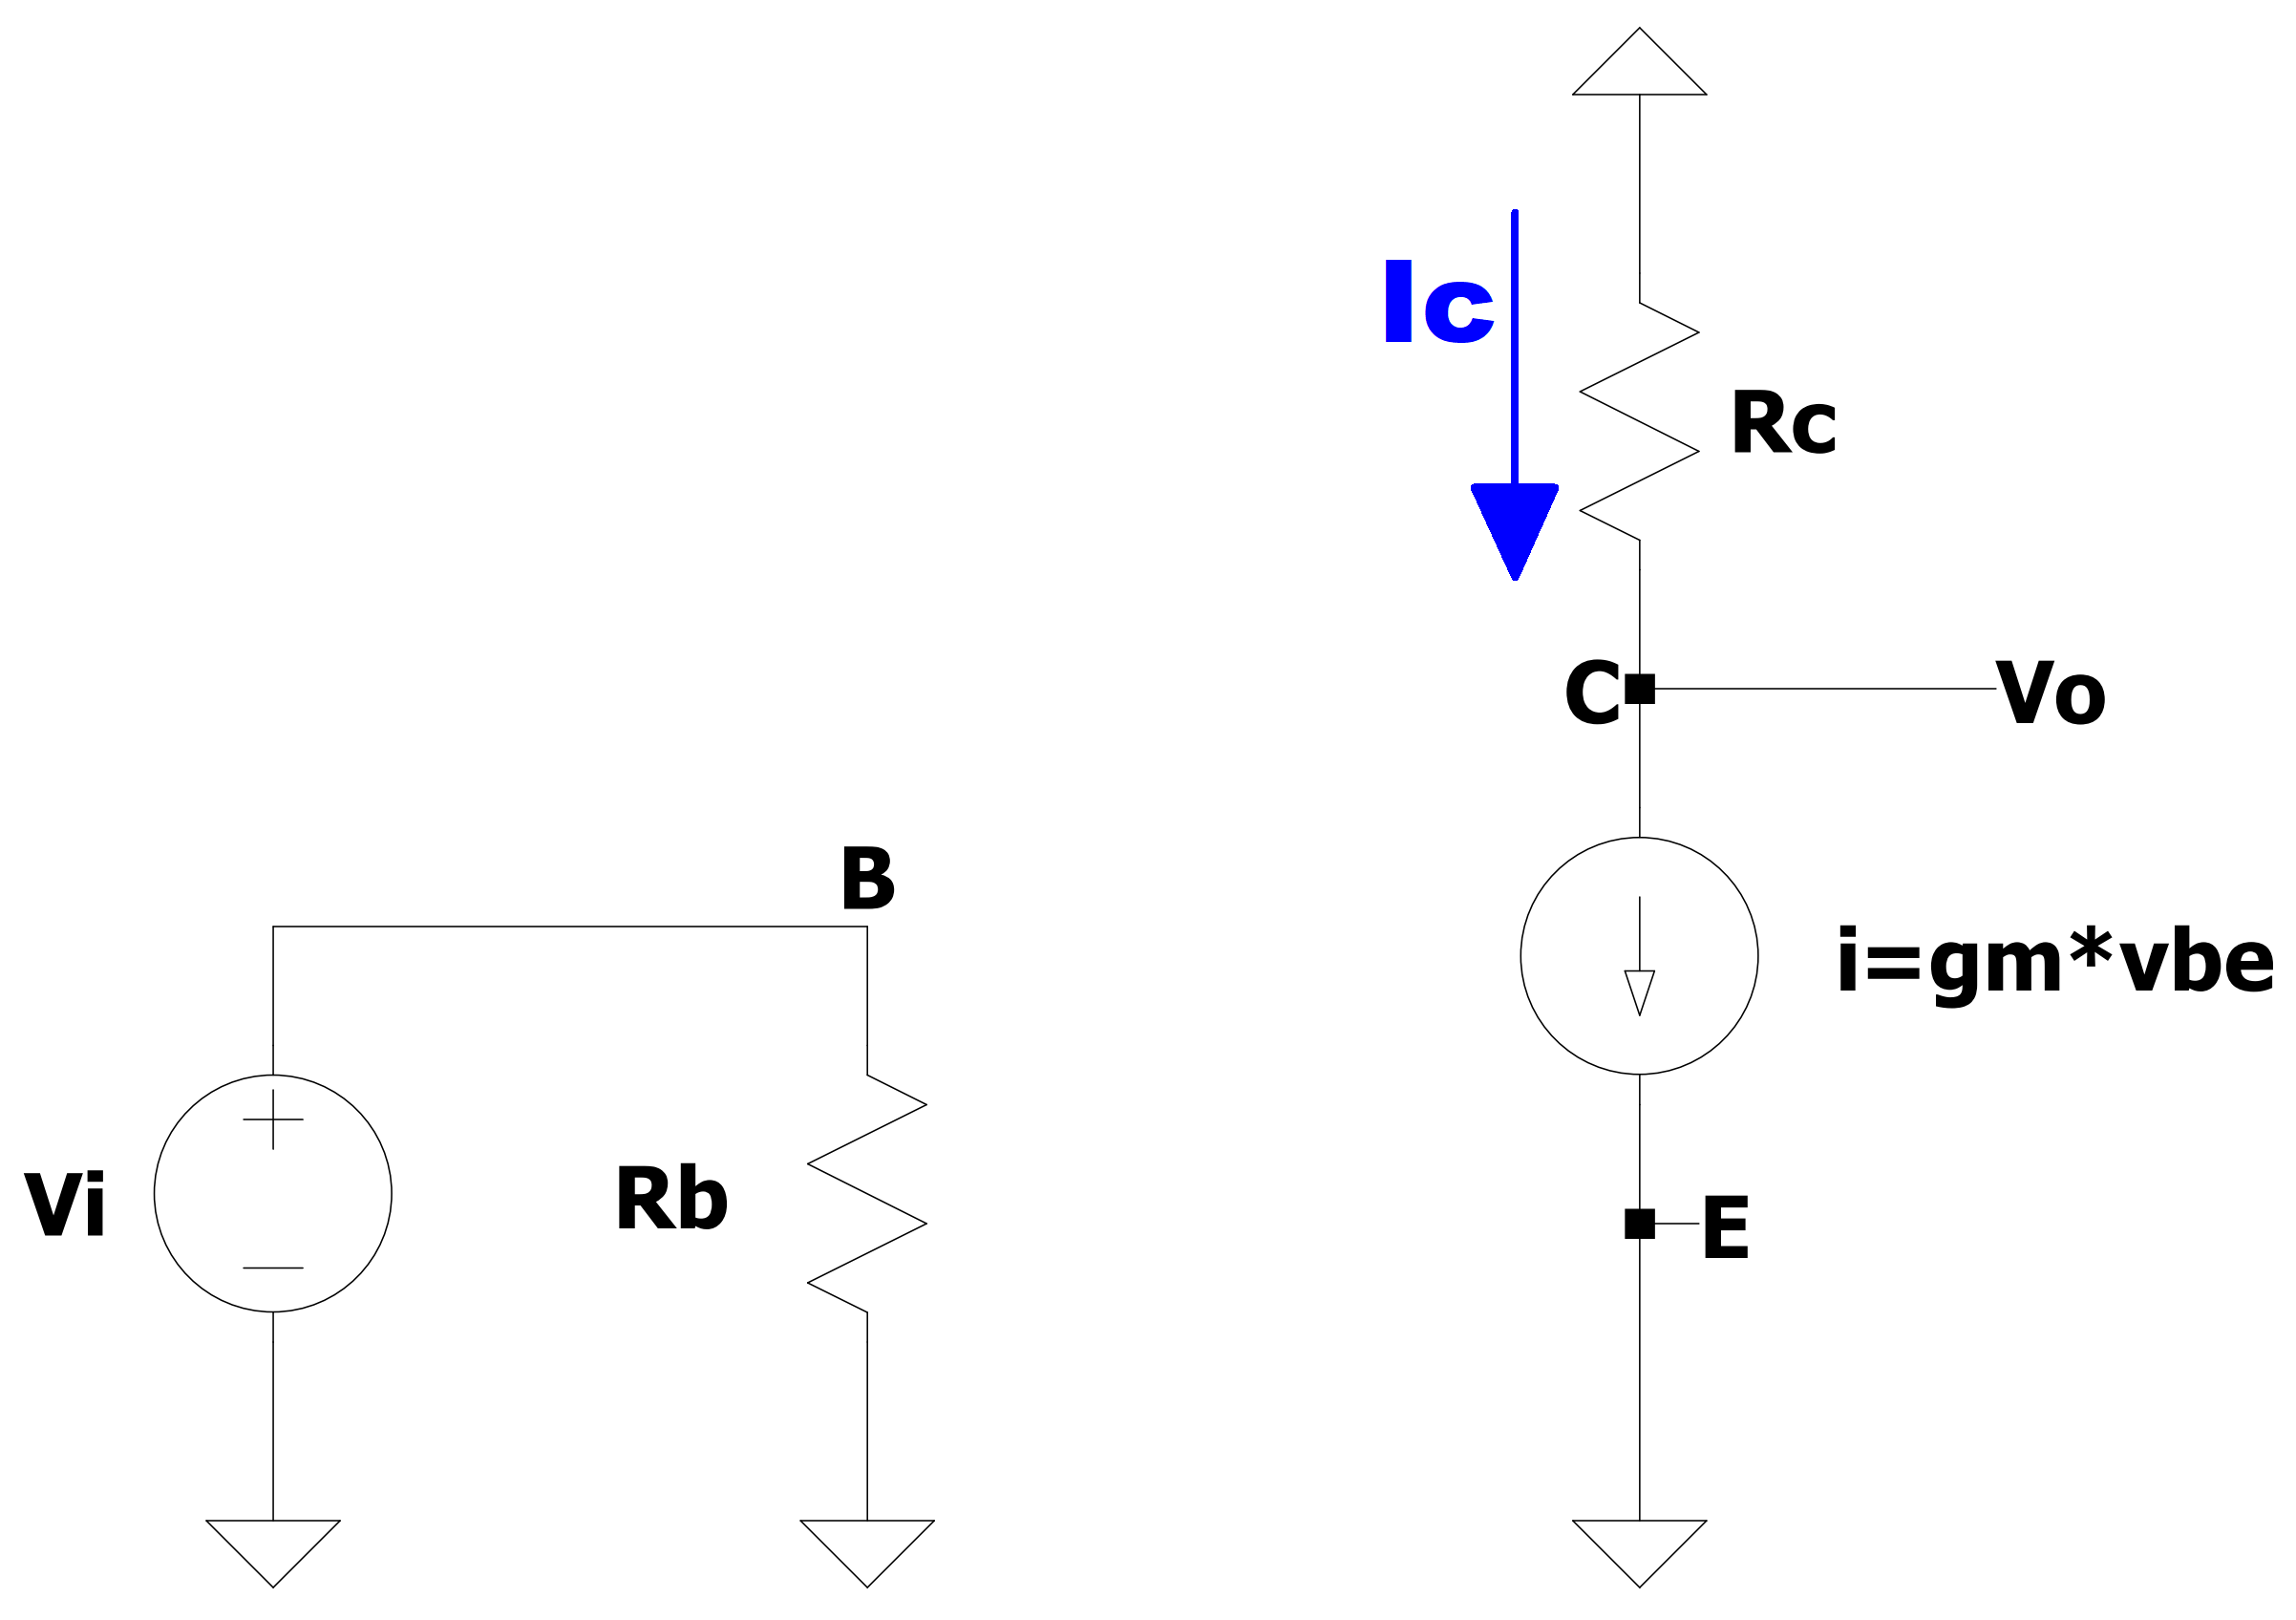
\includegraphics[height=8.7cm]{immagini/CEv1_ps}
\caption{Schema per l'analisi di piccolo segnale.}
\label{figura:CEv1_ps}
\end{figure}
\\La tensione $v_B$ è pari alla tensione in ingresso $v_i$, dato che nel circuito di sinistra non circola corrente. Per quanto riguarda il circuito di destra, facciamo un bilancio di correnti al nodo del collettore:
\\[2pt]\indent $\displaystyle{i_C=i=g_m v_{BE}=\frac{0V-v_c}{R_C}}$
\\[2pt]Sappiamo però che $v_B=v_i$, $v_C=v_o$ e $v_E=0V$ perché questo nodo si trova a massa. L'equazione precedente si può riscrivere come:
\\[2pt]\indent $\displaystyle{g_m v_i=\frac{-v_o}{R_C}}$
\\[2pt]A questo punto possiamo calcolare facilmente la funzione di trasferimento del circuito, che risulta:
\\[2pt]\indent $\displaystyle{\frac{v_o}{v_i}=-g_m R_C}$
\\[2pt]Dato che solitamente $g_m R_C\gg 1$, il circuito ha un guadagno in tensione, come ci aspettavamo. Il guadagno dipende dalla resistenza $R_C$ e dalla transconduttanza $g_m$. Quest'ultima introduce però alcuni problemi, perché ricordando che la transconduttanza è definita come:
\\[2pt]\indent $\displaystyle{g_m=\frac{I_C}{\Phi_T}}$ e che $\displaystyle{\Phi_T=\frac{k_b\cdot T}{q}}$
\\[2pt]risulta evidente che il guadagno dipende sia dal punto di lavoro del circuito ($I_C$) che dalla temperatura ($T$). Per risolvere il problema, è sufficiente inserire una resistenza fra l'emettitore e massa, ottenendo un \textit{Common Emitter amplifier} con \textit{degenerazione di emettitore}. Questa soluzione sarà presentata nelle sezioni \ref{CEv2_cap} (\textit{Common Emitter amplifier} ad alimentazione duale) e \ref{CEv3_cap} (\textit{Common Emitter amplifier} ad alimentazione singola). 
\\\indent Dalla funzione di trasferimento possiamo già notare che compare un segno meno: questo introdurrà uno sfasamento di 180° fra il segnale d'ingresso e il segnale d'uscita. Gli amplificatori realizzati saranno perciò \textit{invertenti}.
\section{Seconda versione} \label{CEv2_cap}% con degenerazione emitter, alimentazione duale
La prima versione di \textit{Common Emitter amplifier} con degenerazione di emettitore analizzata è quella ad alimentazione duale. Di seguito si riportano lo schema (figura \ref{figura:CEv2}), l'analisi del punto di lavoro e di piccolo segnale, e le misure effettuate su questo circuito. 
\begin{figure}[h]
\centering
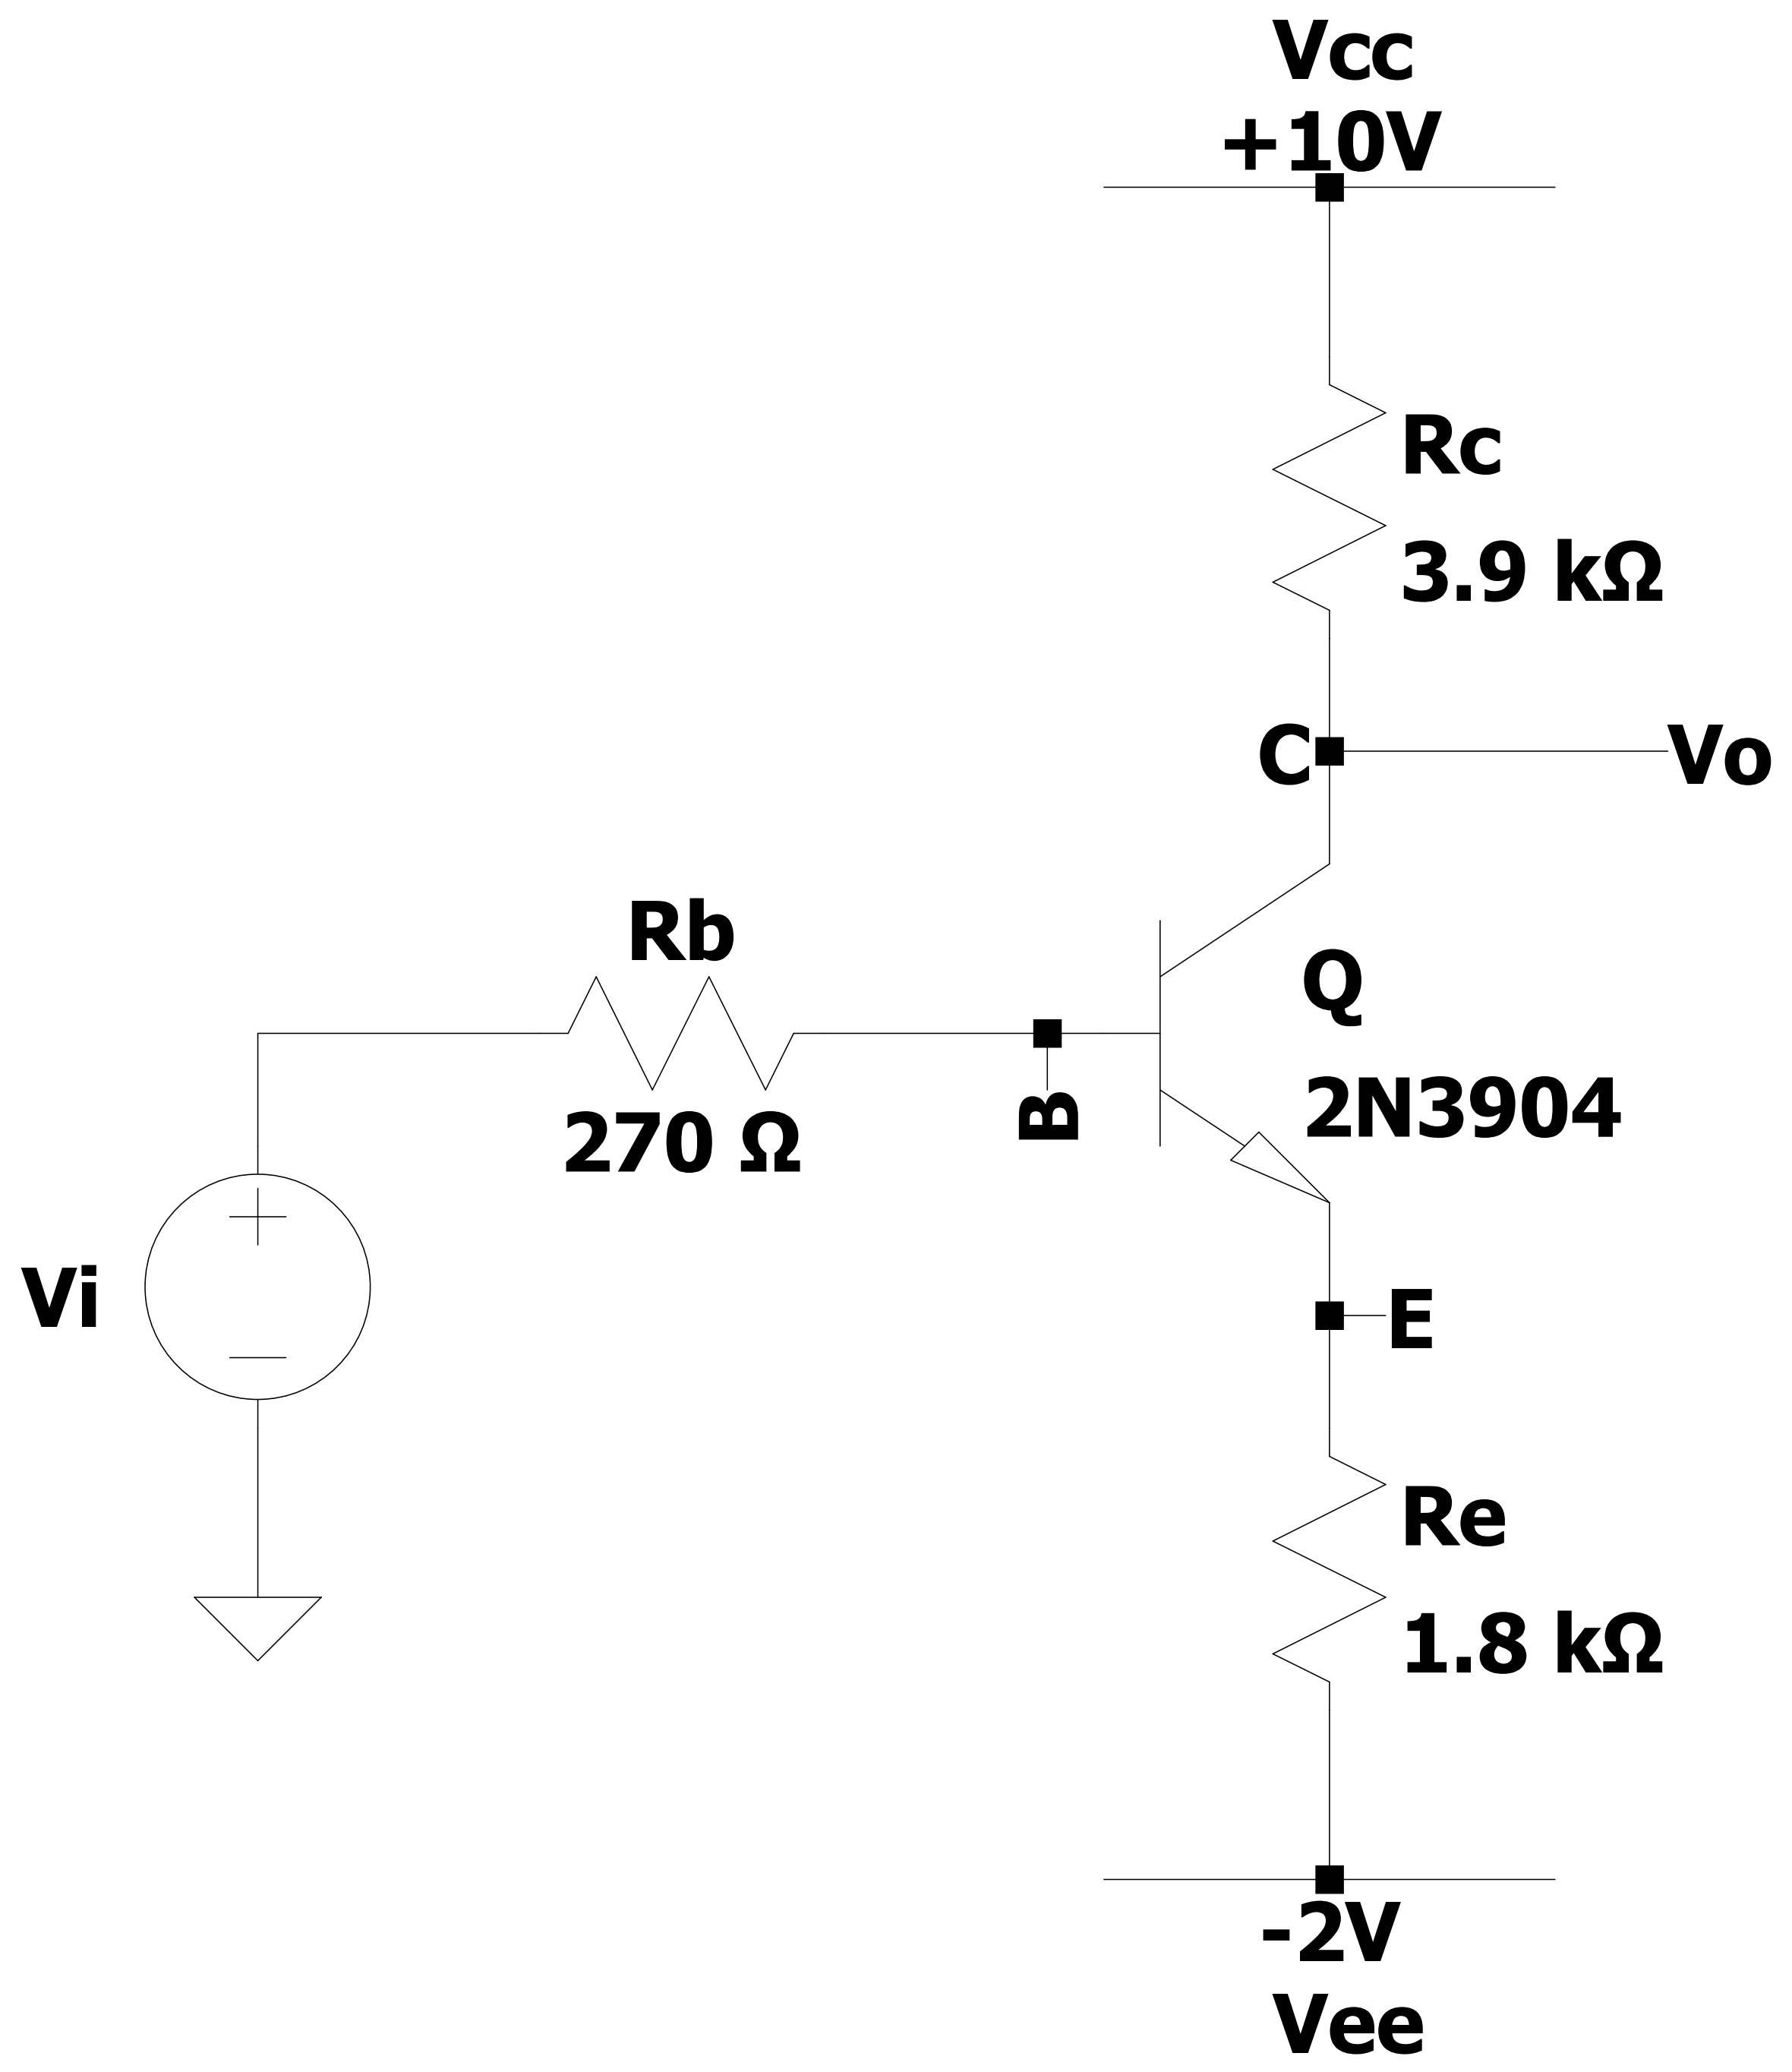
\includegraphics[height=11cm]{immagini/CEv2}
\caption{\textit{Common Emitter amplifier} con degenerazione di emettitore ad alimentazione duale.}
\label{figura:CEv2}
\end{figure}
\subsection{Punto di lavoro} \label{ptolavCEv2}
Per il punto di lavoro è sufficiente sostituire il generatore di segnale con un cortocircuito. Otteniamo lo schema di figura \ref{figura:CEv2_pl}.
\begin{figure}[h]
\centering
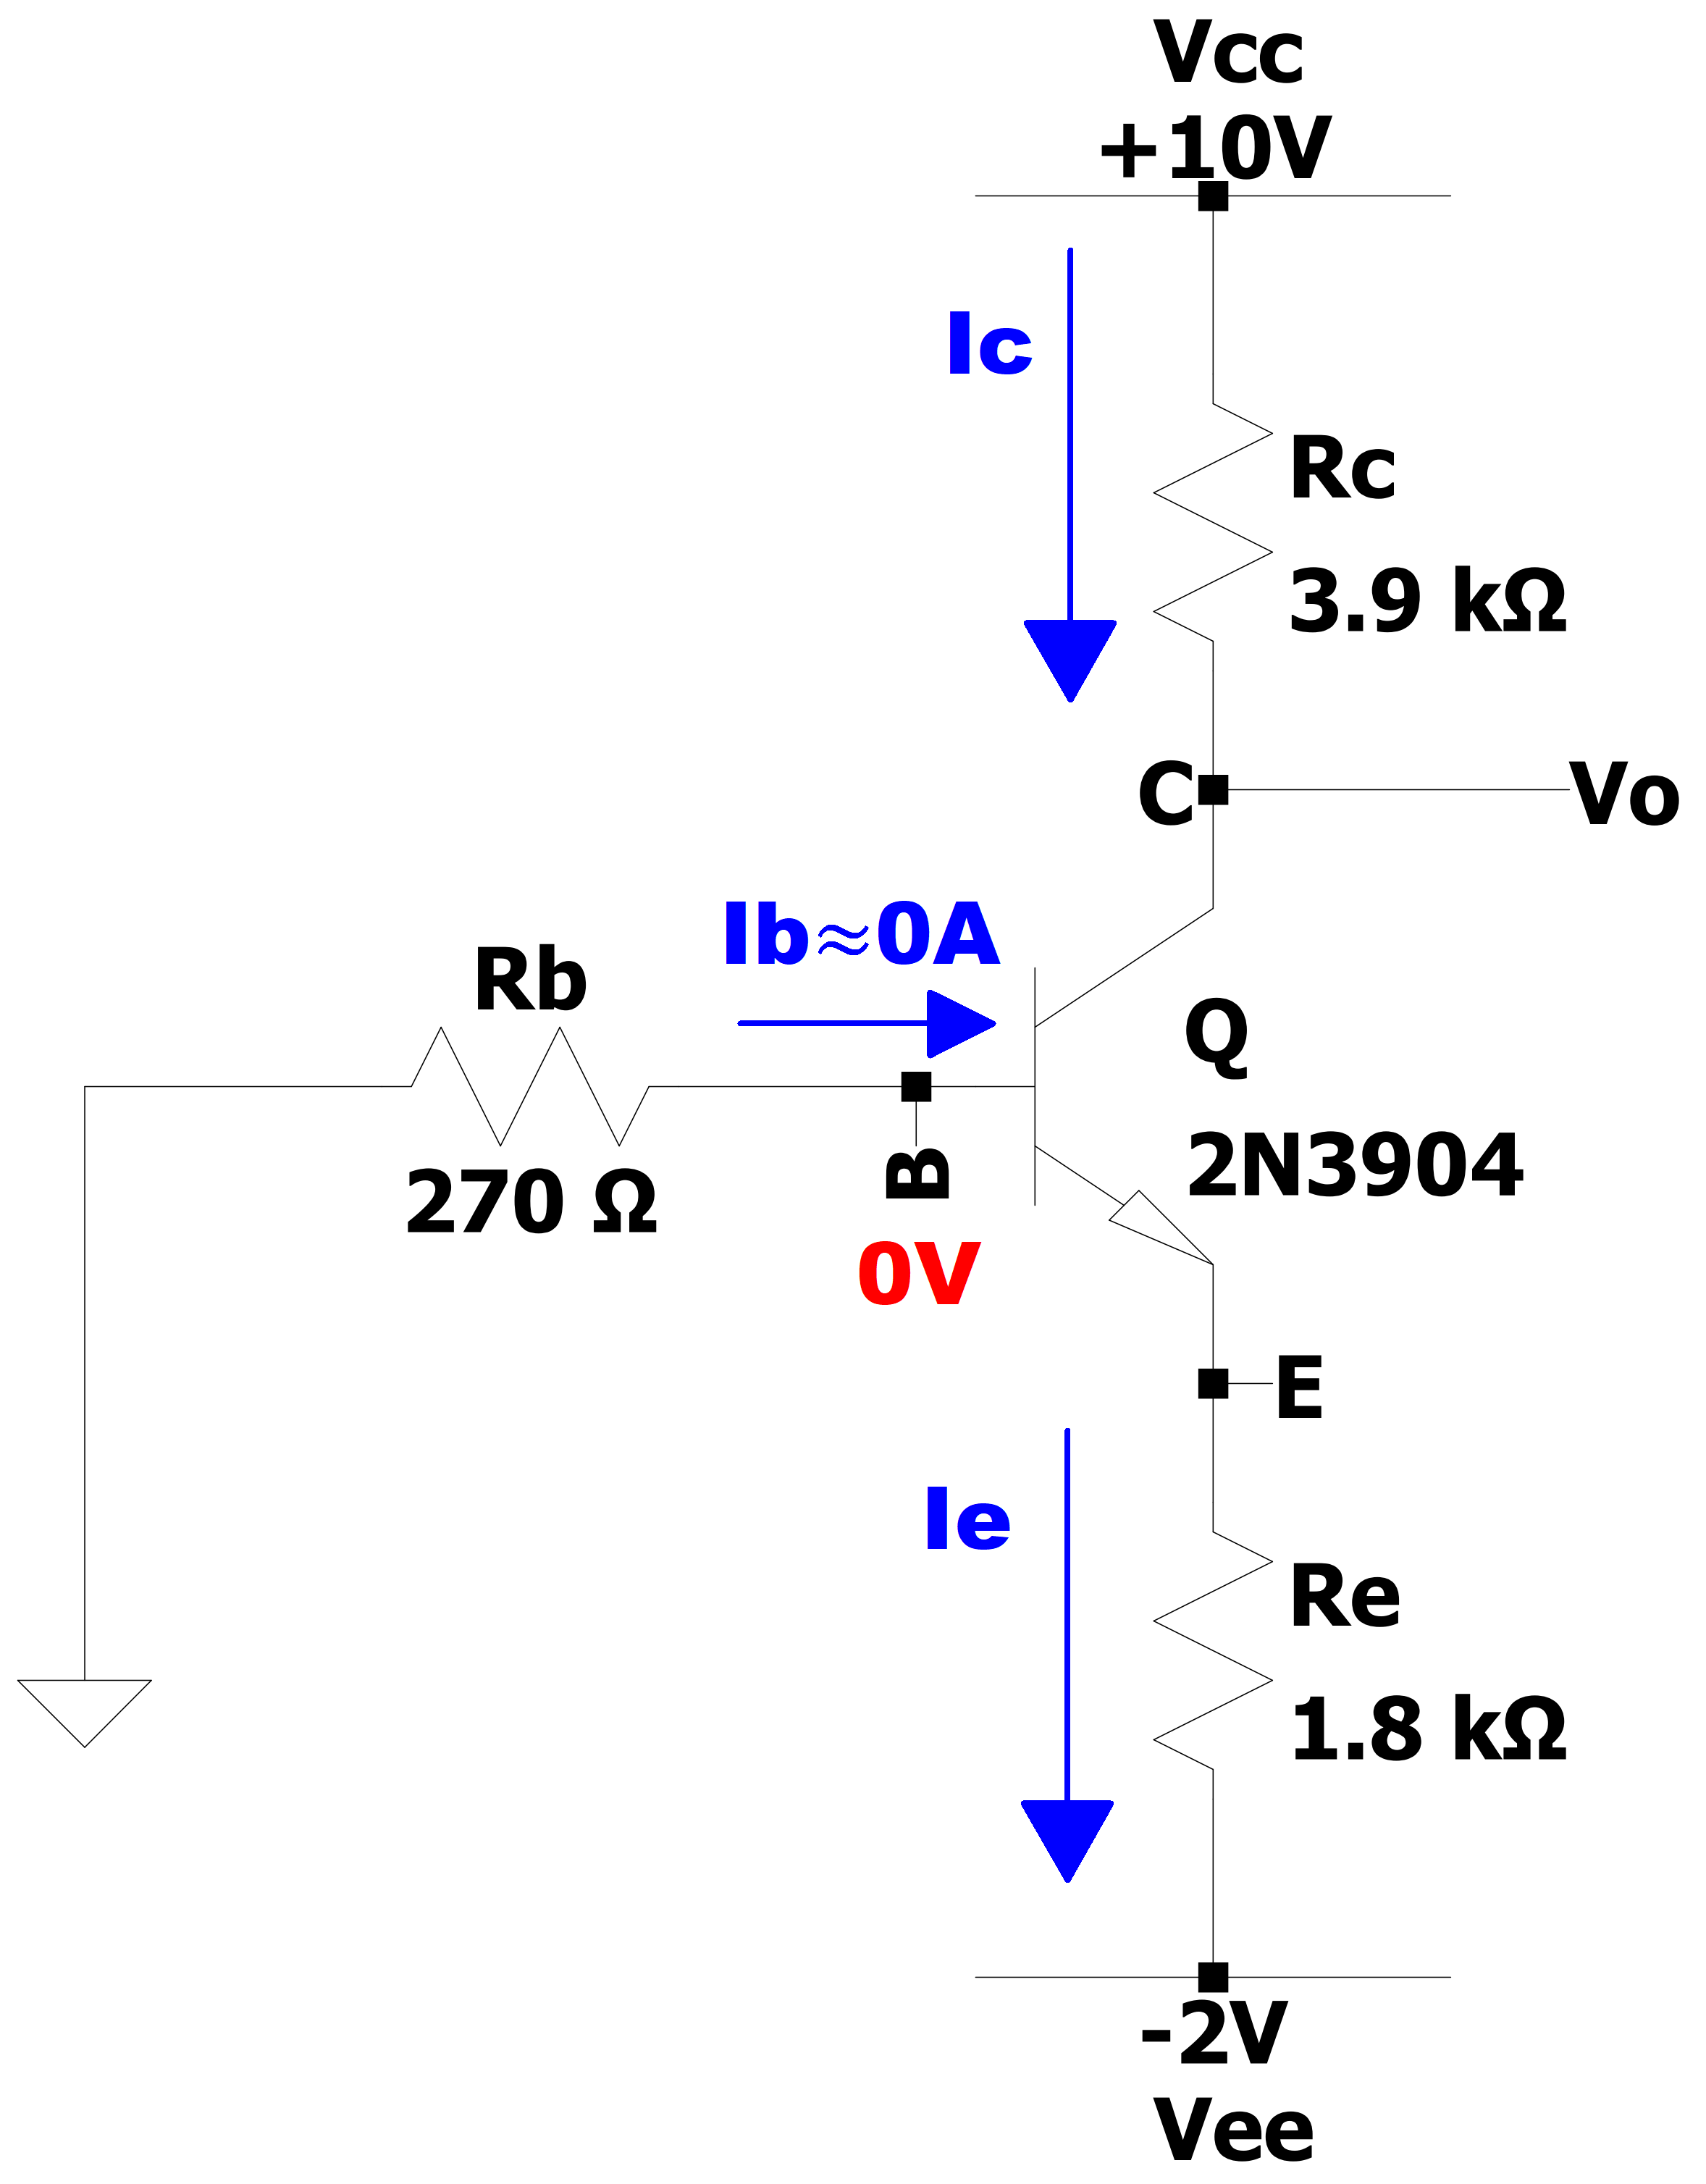
\includegraphics[height=11cm]{immagini/CEv2_pl}
\caption{Schema del circuito per l'analisi del punto di lavoro.}
\label{figura:CEv2_pl}
\end{figure}
\\Nell'analisi utilizziamo il modello ideale del transistor, perciò assumiamo che $\displaystyle{\beta\rightarrow\infty}$ e che $I_{B}=0A$, di conseguenza la corrente che fluisce nella resistenza è nulla, perciò, per la legge di Ohm, sarà nulla anche la caduta di tensione ai suoi capi, quindi si ricava che $V_{B}=0V$. 
\\Suppondendo che il transistor si trovi in regione attiva diretta, la tensione $V_{BE}$ fra la base e l'emettitore è pari a circa +0.7V perché la giunzione è polarizzata direttamente. Dato che sappiamo che $V_{B}=0V$, possiamo calcolare per differenza $V_{E}$, dunque $V_{E}=0V-0.7V=-0.7V$.
\\Calcoliamo la corrente di emettitore con la legge di Ohm: 
\\[2pt]\indent$\displaystyle{V_E-V_{EE}=R_E\cdot I_E \rightarrow I_E=\frac{V_E-V_{EE}}{R_E}=\frac{-0.7V-(-2V)}{1.8k\Omega}=0.722mA}$
\\[2pt]Consideriamo il transistor come se fosse un nodo, otteniamo che $I_C+I_B=I_E$, ma dato che $I_{B}$ è nulla, allora $I_C=I_E=0.722mA$.
\\L'ultima grandezza da determinare è la tensione $V_C$, che è uguale alla tensione $V_o$ dato che l'uscita viene prelevata al collettore. Per ricavarla utilizziamo ancora la legge di Ohm:
\\[2pt]\indent $\displaystyle{V_C=V_{CC}-R_C\cdot I_C= 10V-\SI{3.9}{k\ohm}\cdot 0.722mA=7.184V}$
\\Dato che $V_{CB}>0V$, la giunzione base-collettore è polarizzata inversamente, quindi l'ipotesi che il transistor si trovi in regione attiva diretta è verificata. 
\\Ora che abbiamo risolto il circuito, calcoliamo anche la transconduttanza:
\\[2pt]\indent$\displaystyle{g_m=\frac{I_C}{\Phi_T}=\frac{0.722mA}{26mV}=0.0278\frac{A}{V}}$
\\[3pt]In tabella \ref{table:CEv2_pl} sono riassunte tutte le grandezze ricavate dal punto di lavoro. 
\begin{table}[h]
	\centering
	\begin{tabular}{|c|c|c|c|c|c|c|}
		\hline
		\textbf{V\ped{B}[V]} & \textbf{V\ped{C}[V]} & \textbf{V\ped{E}[V]} & \textbf{I\ped{B}[A]} & \textbf{I\ped{E}[mA]} & \textbf{I\ped{C}[mA]} & \textbf{g\ped{m}[A/V]} \\ 
		\hline
		0 & 7.184 & -0.7 & 0 & 0.722 & 0.722 & 0.0278\\ 
		\hline
	\end{tabular}
\caption{Riassunto delle grandezze ricavate dal punto di lavoro del circuito.}
\label{table:CEv2_pl}
\end{table}
\subsection{Analisi di piccolo segnale} \label{CEv3_pscap}
Terminato il punto di lavoro, passiamo all'analisi per piccolo segnale. Poniamo le due alimentazioni a massa e sostituiamo al transistor il suo modello per piccolo segnale a bassa frequenza. Lo schema è mostrato in figura \ref{figura:CEv2_ps}.
\begin{figure}[h]
\centering
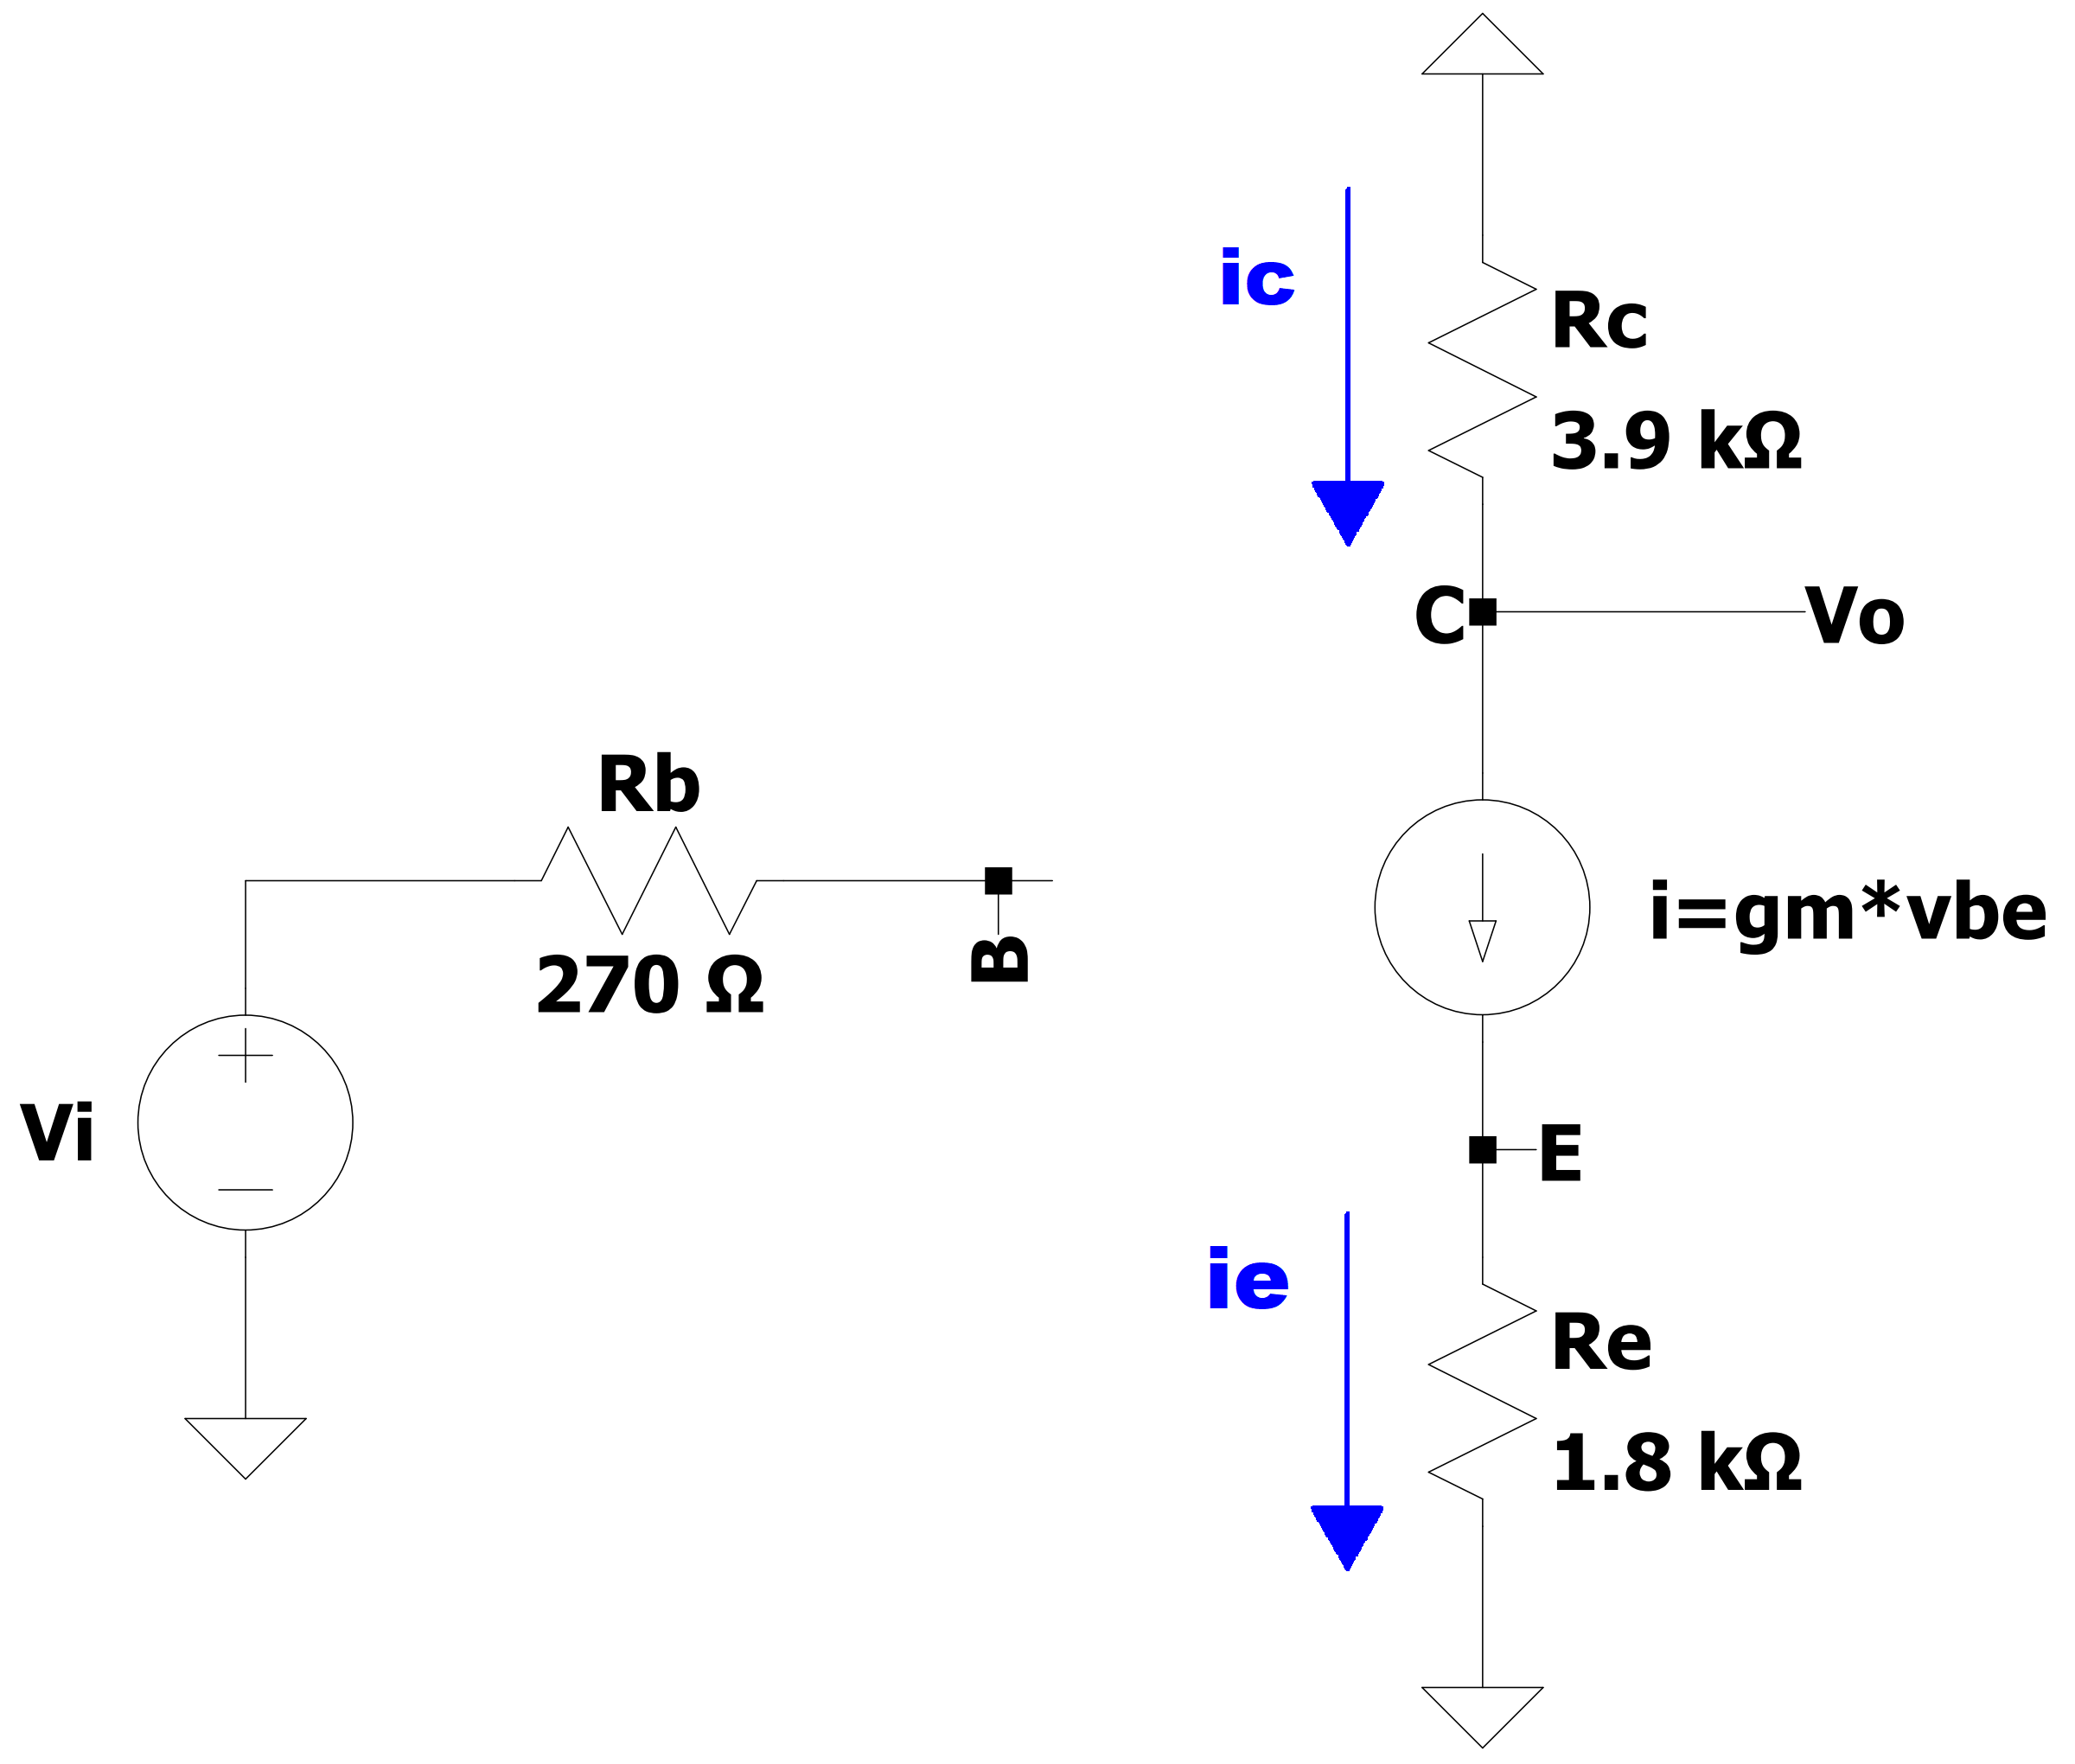
\includegraphics[height=11cm]{immagini/CEv2_ps}
\caption{Schema del circuito per l'analisi di piccolo segnale.}
\label{figura:CEv2_ps}
\end{figure}
\\Dato che la base del transistor è isolata, nel circuito di sinistra non circola corrente, perciò non c'è caduta di tensione sulla resistenza $R_B$, quindi la tensione $v_B$ risulta pari alla tensione applicata in ingresso con il generatore $v_i$.
\\Eseguendo un bilancio di correnti al collettore otteniamo:
\\[2pt]\indent$i_C=i=g_m\cdot v_{BE}$ ma $\displaystyle{i_C=-\frac{v_C}{R_C}}$ per la legge di Ohm $\displaystyle{\rightarrow -\frac{v_C}{R_C}=g_m\cdot v_{BE}}$
\\[2pt]Dato che l'uscita è prelevata al collettore, $v_o=v_C$, perciò ricaviamo $v_o$ dall'equazione precedente:
\begin{equation}
v_o=-g_m R_C\cdot v_{BE}
\label{f1}
\end{equation}
Sappiamo già che $v_B$ è uguale a $v_i$, dobbiamo ricavare $v_E$. Trattiamo il transistor come se fosse un nodo e facciamo un bilancio di correnti:
\\[2pt]\indent$\displaystyle{-\frac{v_o}{R_C}=\frac{v_E}{R_E}\rightarrow v_E=-\frac{R_E}{R_C}\cdot v_o}$ 
\\[2pt]Sostituiamo le grandezze note nell'equazione \eqref{f1}. Otteniamo:
\\[2pt]\indent$\displaystyle{v_o=-g_mR_C\cdot v_i+g_mR_C \left( -\frac{R_E}{R_C}\cdot v_o \right)=-g_mR_C\cdot v_i-g_mR_E\cdot v_o}$
\\[2pt]Dall'equazione precedente si può ricavare la funzione di trasferimento del circuito, che risulta:
\\[2pt]\indent $\displaystyle{\frac{v_o}{v_i}=-\frac{g_mR_C}{1+g_mR_E}\simeq -\frac{R_C}{R_E}}$ per $g_mR_E\gg 1$
\\[2pt]Rispetto alla soluzione già trattata nella sezione \ref{CEv1_cap}, il guadagno di questo circuito dipende solo debolmente dalla transconduttanza, il cui contributo è molto spesso trascurabile. Nella funzione di trasferimento rimane il segno meno, perciò il segnale in uscita sarà sfasato di 180° rispetto al segnale in ingresso: l'amplificatore realizzato sarà pertanto invertente. 
\\\indent Il guadagno dipende dal rapporto fra la resistenza di collettore e la resistenza di emettitore: se $R_C<R_E$ il circuito attenua il segnale in ingresso, quindi otteniamo un attenuatore; se $R_C>R_E$ il segnale viene amplificato, perciò il circuito è un amplificatore; infine, se $R_C=R_E$ il circuito ha guadagno unitario, di conseguenza si comporta come un buffer. Nel nostro circuito, ci aspettiamo un guadagno, in modulo, di:
\\[2pt]\indent$\displaystyle{\frac{R_C}{R_E}=\frac{\SI{3.9}{k\ohm}}{\SI{1.8}{k\ohm}}\simeq 2.17}$
\subsection{Componenti, strumenti e misure} 
Il circuito, mostrato in figura \ref{figura:fotoCEv2_pl} con le connessioni utilizzate per lo studio del punto di lavoro, è stato realizzato su una breadboard utilizzando questi componenti:
\begin{itemize}
\item transistor bipolare NPN 2N3904;
\item una resistenza da \SI{270}{\ohm} per $R_B$;
\item una resistenza da \SI{3.9}{k\ohm} per $R_C$;
\item una resistenza da \SI{1.8}{k\ohm} per $R_E$.
\end{itemize}
\begin{figure}[h]
\centering
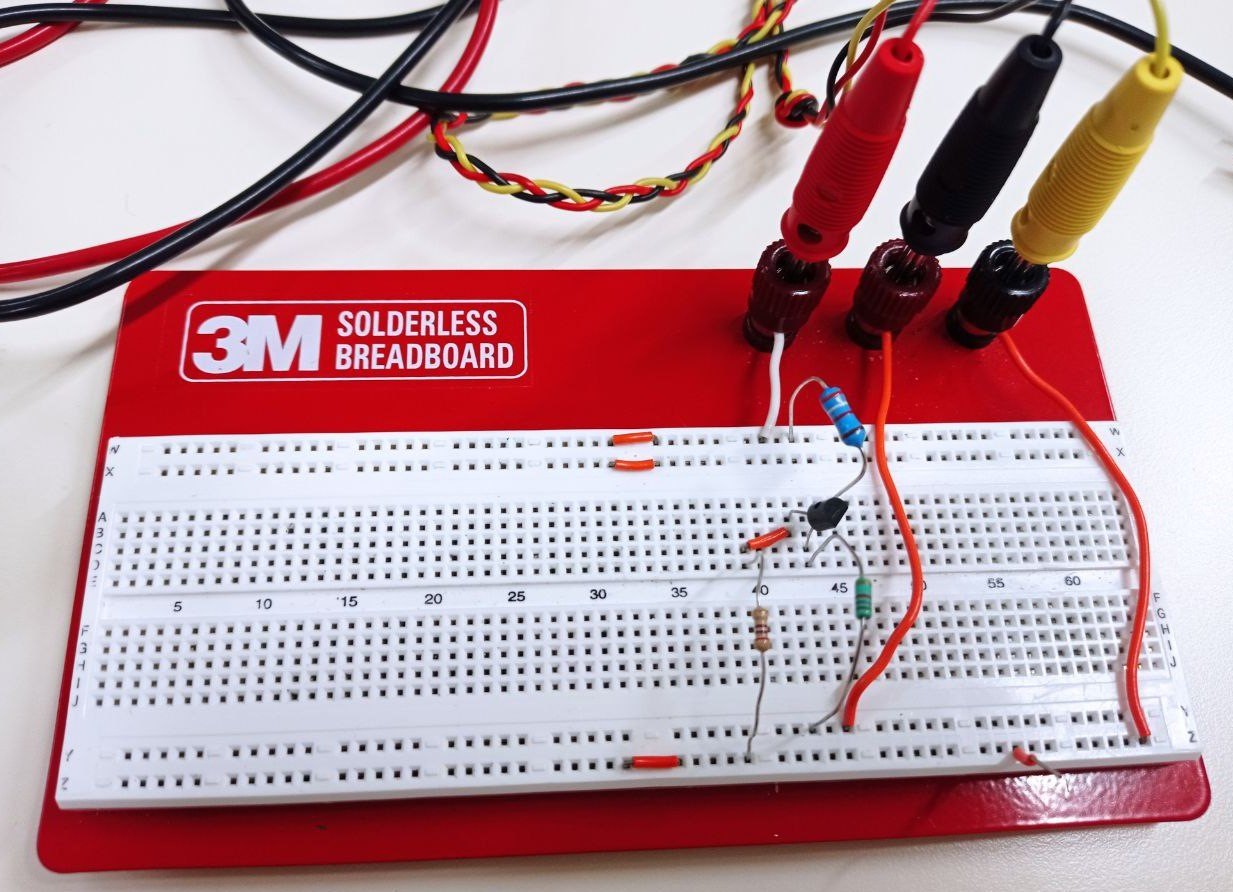
\includegraphics[height=8.9cm]{immagini/fotoCEv2_pl}
\caption{\textit{Common Emitter amplifier} con le connessioni per lo studio del punto di lavoro.}
\label{figura:fotoCEv2_pl}
\end{figure}
Per le misure e le analisi, sono stati utilizzati i seguenti strumenti:
\begin{itemize}
\item alimentatore da banco, con alimentazione positiva impostata a 10V ed alimentazione negativa a -2V, entrambe con limite in corrente di 50mA;
\item generatore di forme d'onda;
\item multimetro da banco;
\item oscilloscopio a due canali.
\end{itemize}
Per prima cosa, con il multimetro si sono misurati i valori delle resistenze ed i valori delle tensioni delle giunzioni p-n del transistor. I valori ottenuti sono mostrati in tabella \ref{table:CEv2_comp}.
\begin{table}[h]
	\centering
	\begin{tabular}{|c|c|c|}
	\cline{2-3} 
	\multicolumn{1}{c|}{} & \textbf{Valore nominale} & \textbf{Valore misurato}\\ 
		%\hline
		%{} & \textbf{Valore nominale} & \textbf{Valore misurato} \\ 
		\hline
		$\mathbf{R_B}$ & \SI{270}{\ohm} & \SI{270}{\ohm} \\ 
		\hline
		$\mathbf{R_C}$& \SI{3.9}{k\ohm} & \SI{3.907}{k\ohm} \\ 
		\hline
		$\mathbf{R_E}$& \SI{1.8}{k\ohm} & \SI{1.807}{k\ohm} \\ 
		\hline
		$\mathbf{V_{BE}}$& $\mathrm{ \simeq0.7V}$ & 0.699V \\ 
		\hline
		$\mathbf{V_{BC}}$& $\mathrm{ \simeq0.7V}$  & 0.659V \\ 
		\hline
	\end{tabular}
\caption{Grandezze misurate prima di realizzare il circuito.}
\label{table:CEv2_comp}
\end{table}
\\Dopo aver posizionato tutti i componenti sulla breadboard, è stato fatto lo studio del punto di lavoro del circuito. Non è stato applicato il segnale e il terminale della resistenza $R_B$ non connesso alla base del transistor è stato collegato a massa. Il circuito risultante è quello già incontrato nella figura \ref{figura:fotoCEv2_pl}.
\\\indent Abbiamo misurato le tensioni dei tre terminali del transistor, poi abbiamo ricavato le correnti di tutti i rami utlilizzando la legge di Ohm. Infine, abbiamo verificato con la legge di Kirchhoff che il bilancio delle correnti del transistor, visto come un nodo, era rispettato. I risultati sono riportati in tabella \ref{table:EFv1_pl_mis}. 
\begin{table}[h]
	\centering
	\begin{tabular}{|c|c|c|c|c|c|c|}
		\hline
		\textbf{V\ped{B}[mV]} & \textbf{V\ped{C}[V]} & \textbf{V\ped{E}[V]} & \textbf{I\ped{B}[mA]} & \textbf{I\ped{E}[mA]} & \textbf{I\ped{C}[mA]} & \textbf{g\ped{m}[A/V]} \\ 
		\hline
		-1.167 & 7.106 & -0.653 & 0.004 & 0.745 & 0.741 & 0.0287\\ 
		\hline
	\end{tabular}
\caption{Grandezze misurate dallo studio del punto di lavoro del circuito.}
\label{table:EFv1_pl_mis}
\end{table}
\\I valori ottenuti sono confrontabili con i risultati teorici calcolati nella sezione \ref{ptolavCEv2}. Come succede anche per i circuiti già analizzati, sia $V_B$ che $I_B$ non sono nulle, ma il loro valore (in modulo) è molto piccolo, perciò nel punto di lavoro è ragionevole trascurarle.
\\\indent Dalla legge di Kirchhoff abbiamo che $I_B+I_C=I_E\rightarrow 0.004mA+0.741mA=0.745mA$, ovvero il bilancio delle correnti sul transistor è verificato.
\\Il guadagno che ci aspettiamo è:
\\[2pt]\indent$\displaystyle{\frac{R_C}{R_E}=\frac{\SI{3.907}{k\ohm}}{\SI{1.807}{k\ohm}}= 2.16}$
\\[2pt]ovvero 0.5\% in meno del guadagno teorico.
\\Applichiamo in ingresso un segnale sinusoidale con frequenza $f=\SI{1}{k\hertz}$ e tensione picco-picco $V_{PP}$ di 1V. La tensione in ingresso e la tensione in uscita sono state visualizzate collegando opportunamente le sonde dell'oscilloscopio, in figura \ref{figura:oscillo4} è mostrato il grafico dei due segnali accoppiati in AC mentre in figura \ref{figura:oscillo5} l'ingresso e l'uscita sono accoppiate in DC.
\begin{figure}[h]
\centering
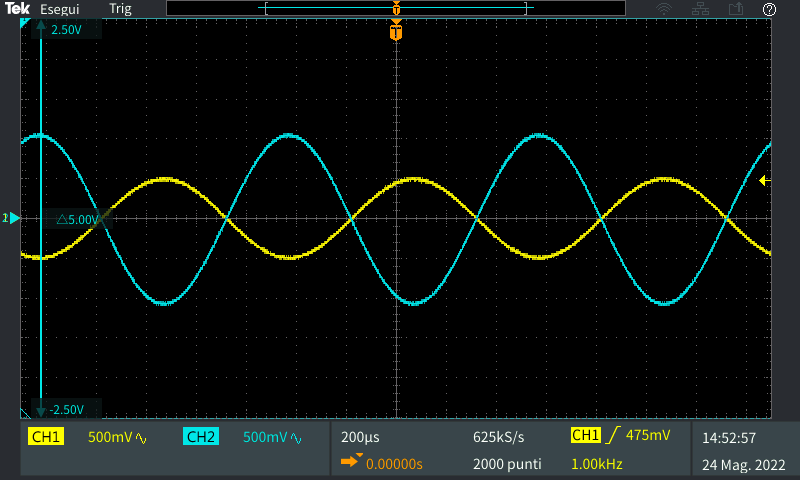
\includegraphics[height=8cm]{immagini/oscillo4}
\caption{Grafico della tensione in ingresso (CH1) e della tensione in uscita (CH2) accoppiate in AC.}
\label{figura:oscillo4}
\end{figure}
\begin{figure}[h!]
\centering
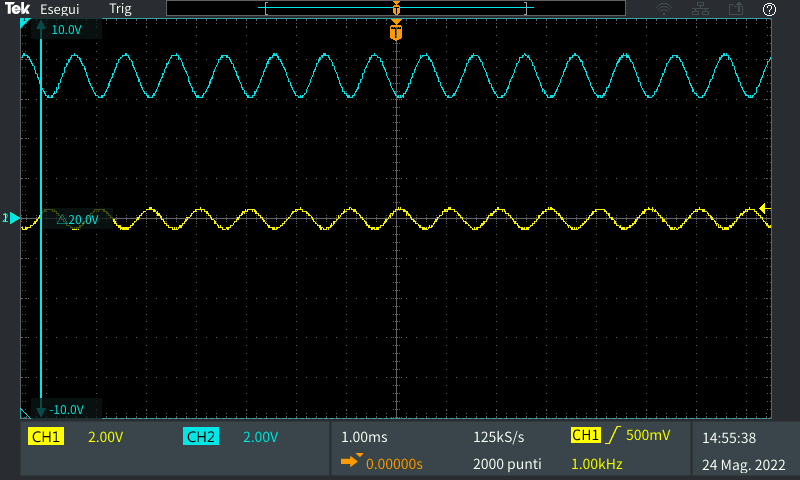
\includegraphics[height=8cm]{immagini/oscillo5}
\caption{Grafico della tensione in ingresso (CH1) e della tensione in uscita (CH2) accoppiate in DC.}
\label{figura:oscillo5}
\end{figure}
\\\\Dai due grafici è evidente che l'amplificatore inverte l'ingresso, perché i due segnali sono in controfase: quando l'ingresso è positivo l'uscita è negativa e viceversa. L'uscita è circa il doppio, in modulo, del segnale applicato in ingresso. 
\section{Terza versione} \label{CEv3_cap} % con degenerazione emitter, alimentazione singola (in piccolo segnale aggiungi già il condensatore)
Dopo aver analizzato il \textit{Common Emitter amplifier} ad alimentazione duale, abbiamo modificato questo circuito per giungere ad una versione ad alimentazione singola. L'alimentazione negativa è stata sostituita con la massa, successivamente abbiamo applicato un partitore di tensione alla base del transistor e abbiamo inserito un condensatore fra il segnale e la base, per evitare di incontrare le problematiche già riscontrate nella costruzione dell'\textit{Emitter follower} ad alimentazione singola e discusse nella sezione \ref{EFv2cap}. Il circuito completo è riportato in figura \ref{figura:CEv3}.
\begin{figure}[h]
\centering
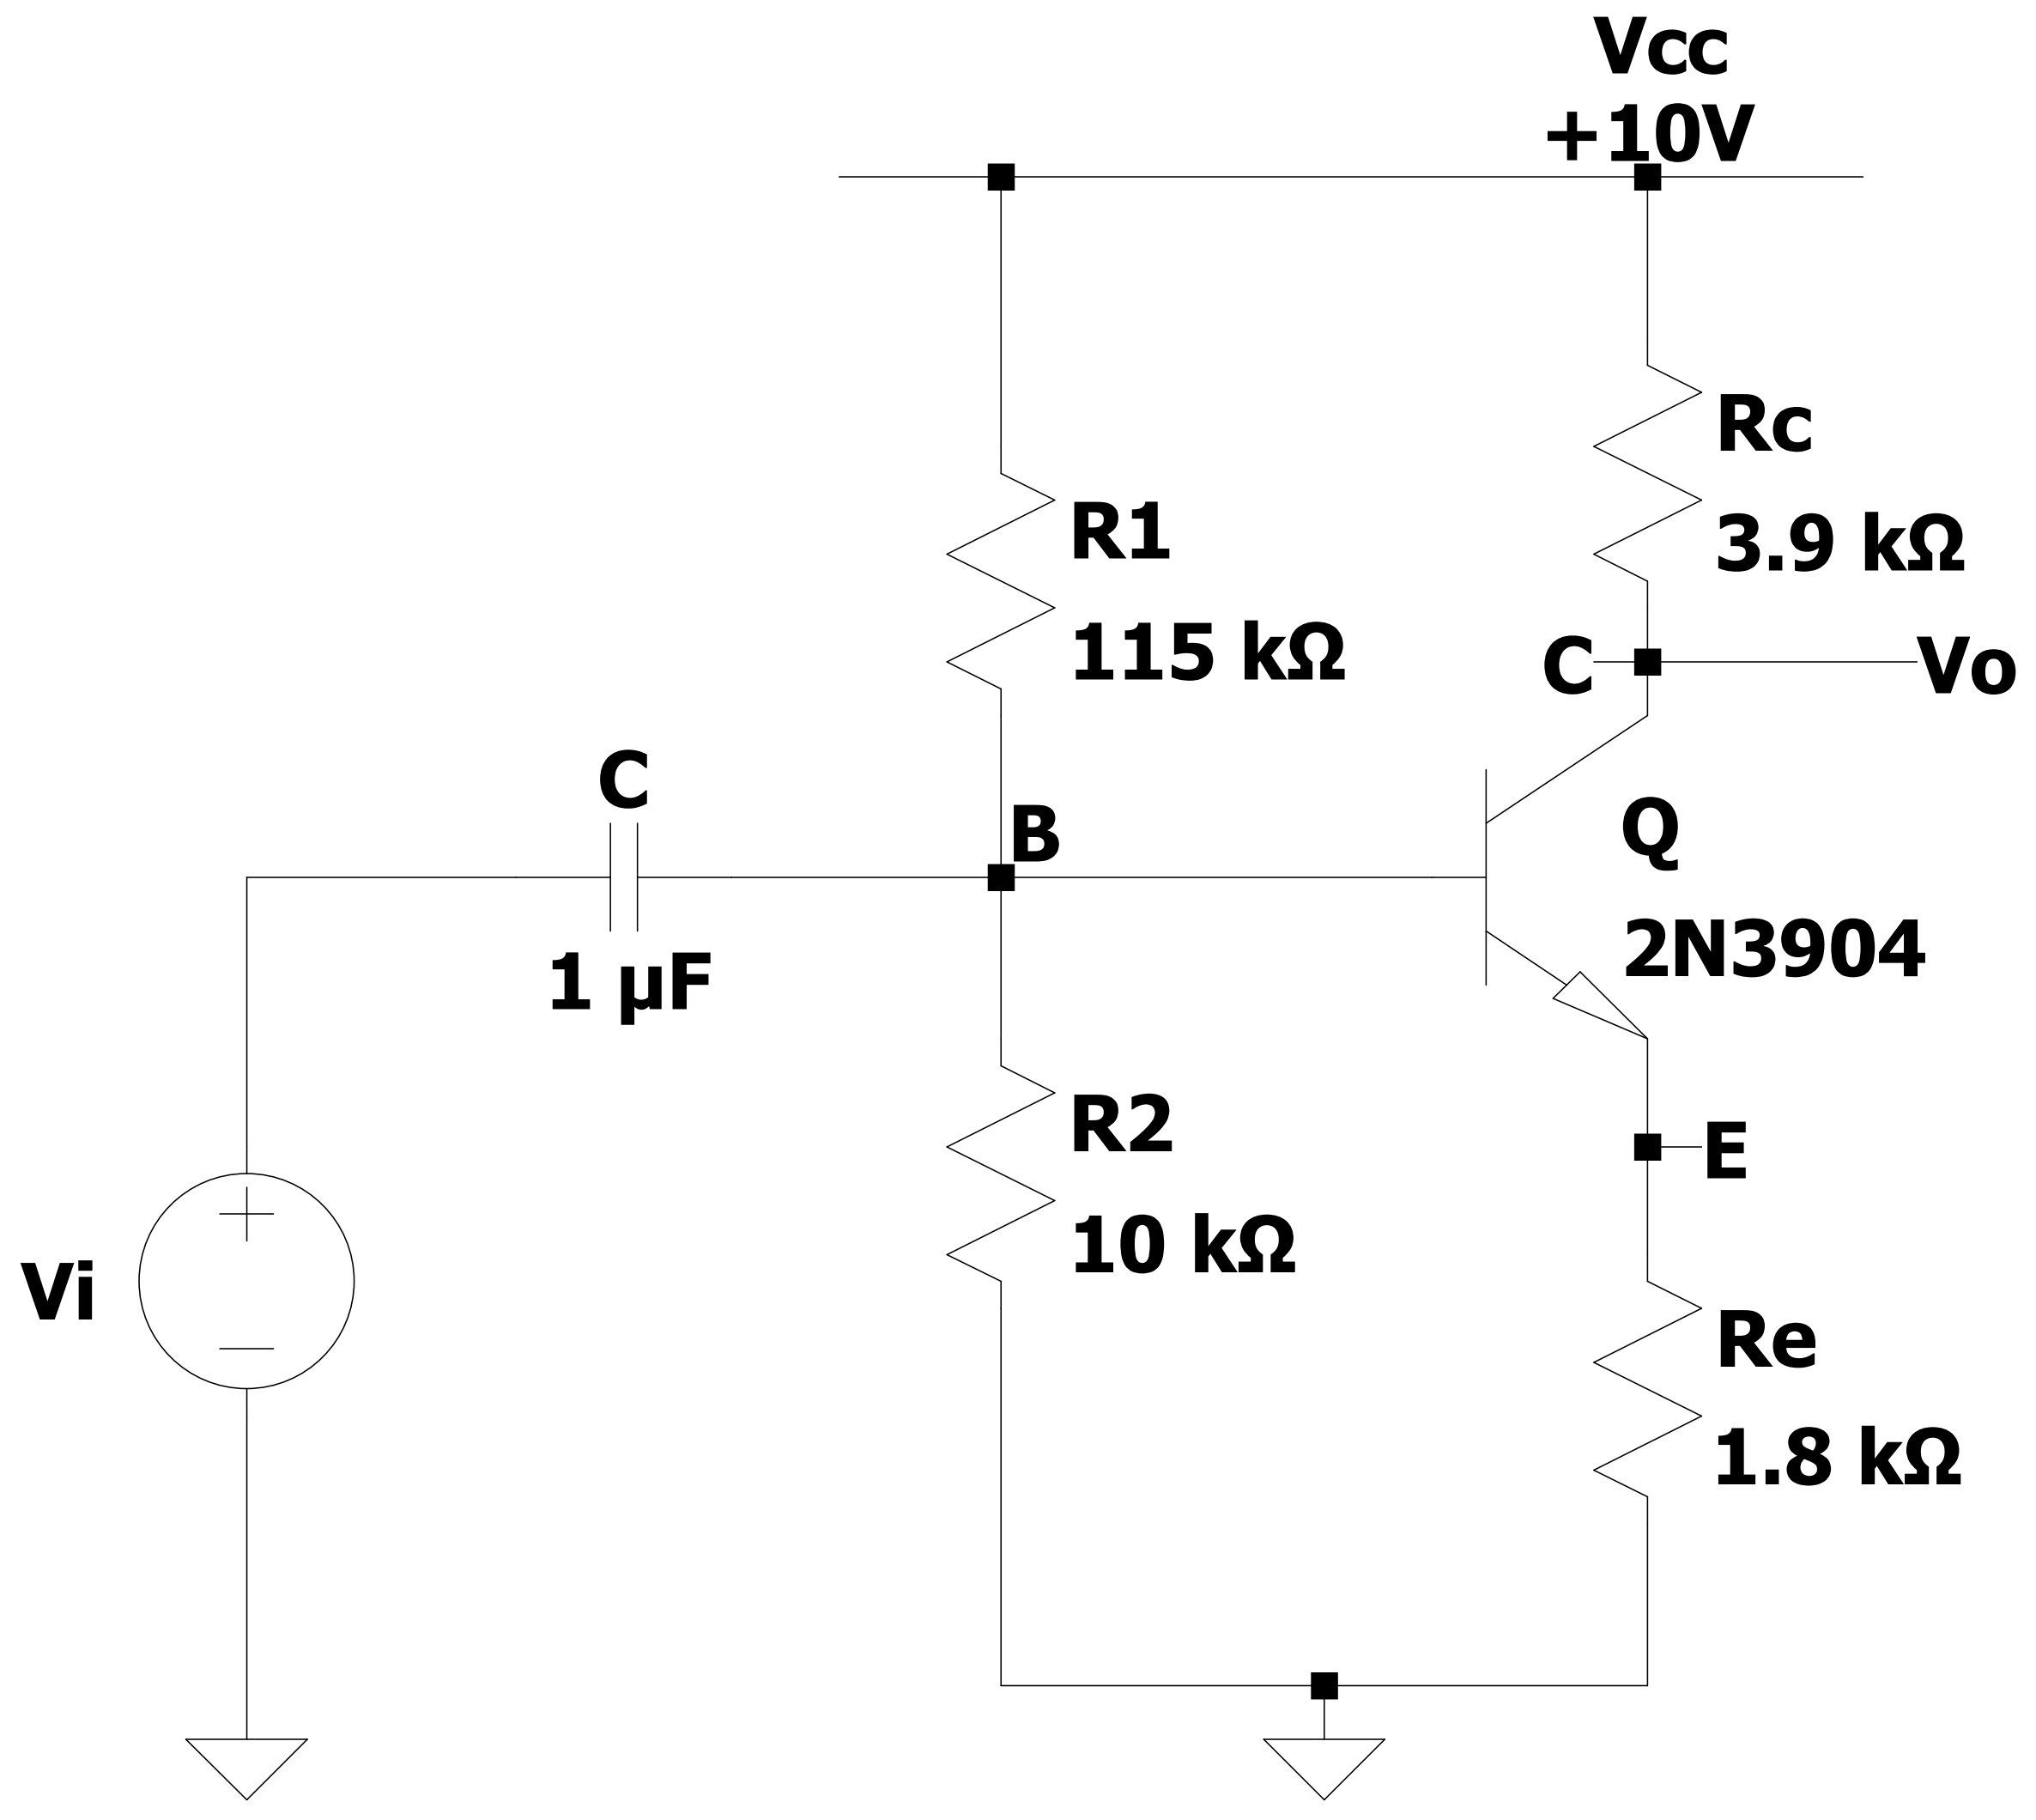
\includegraphics[height=10cm]{immagini/CEv3}
\caption{Schema del \textit{Common Emitter amplifier} ad alimentazione singola.}
\label{figura:CEv3}
\end{figure}
\subsection{Punto di lavoro} \label{CEv3_plcap}
Il punto di lavoro è molto simile a quello del \textit{Common Emitter amplifier} con degenerazione di emettitore ad alimentazione duale analizzato nella sezione \ref{ptolavCEv2}. Il generatore di segnale è sostituito con un cortocircuito ed il condensatore con un circuito aperto. Otteniamo lo schema di figura \ref{figura:CEv3_pl}.
\begin{figure}[h]
\centering
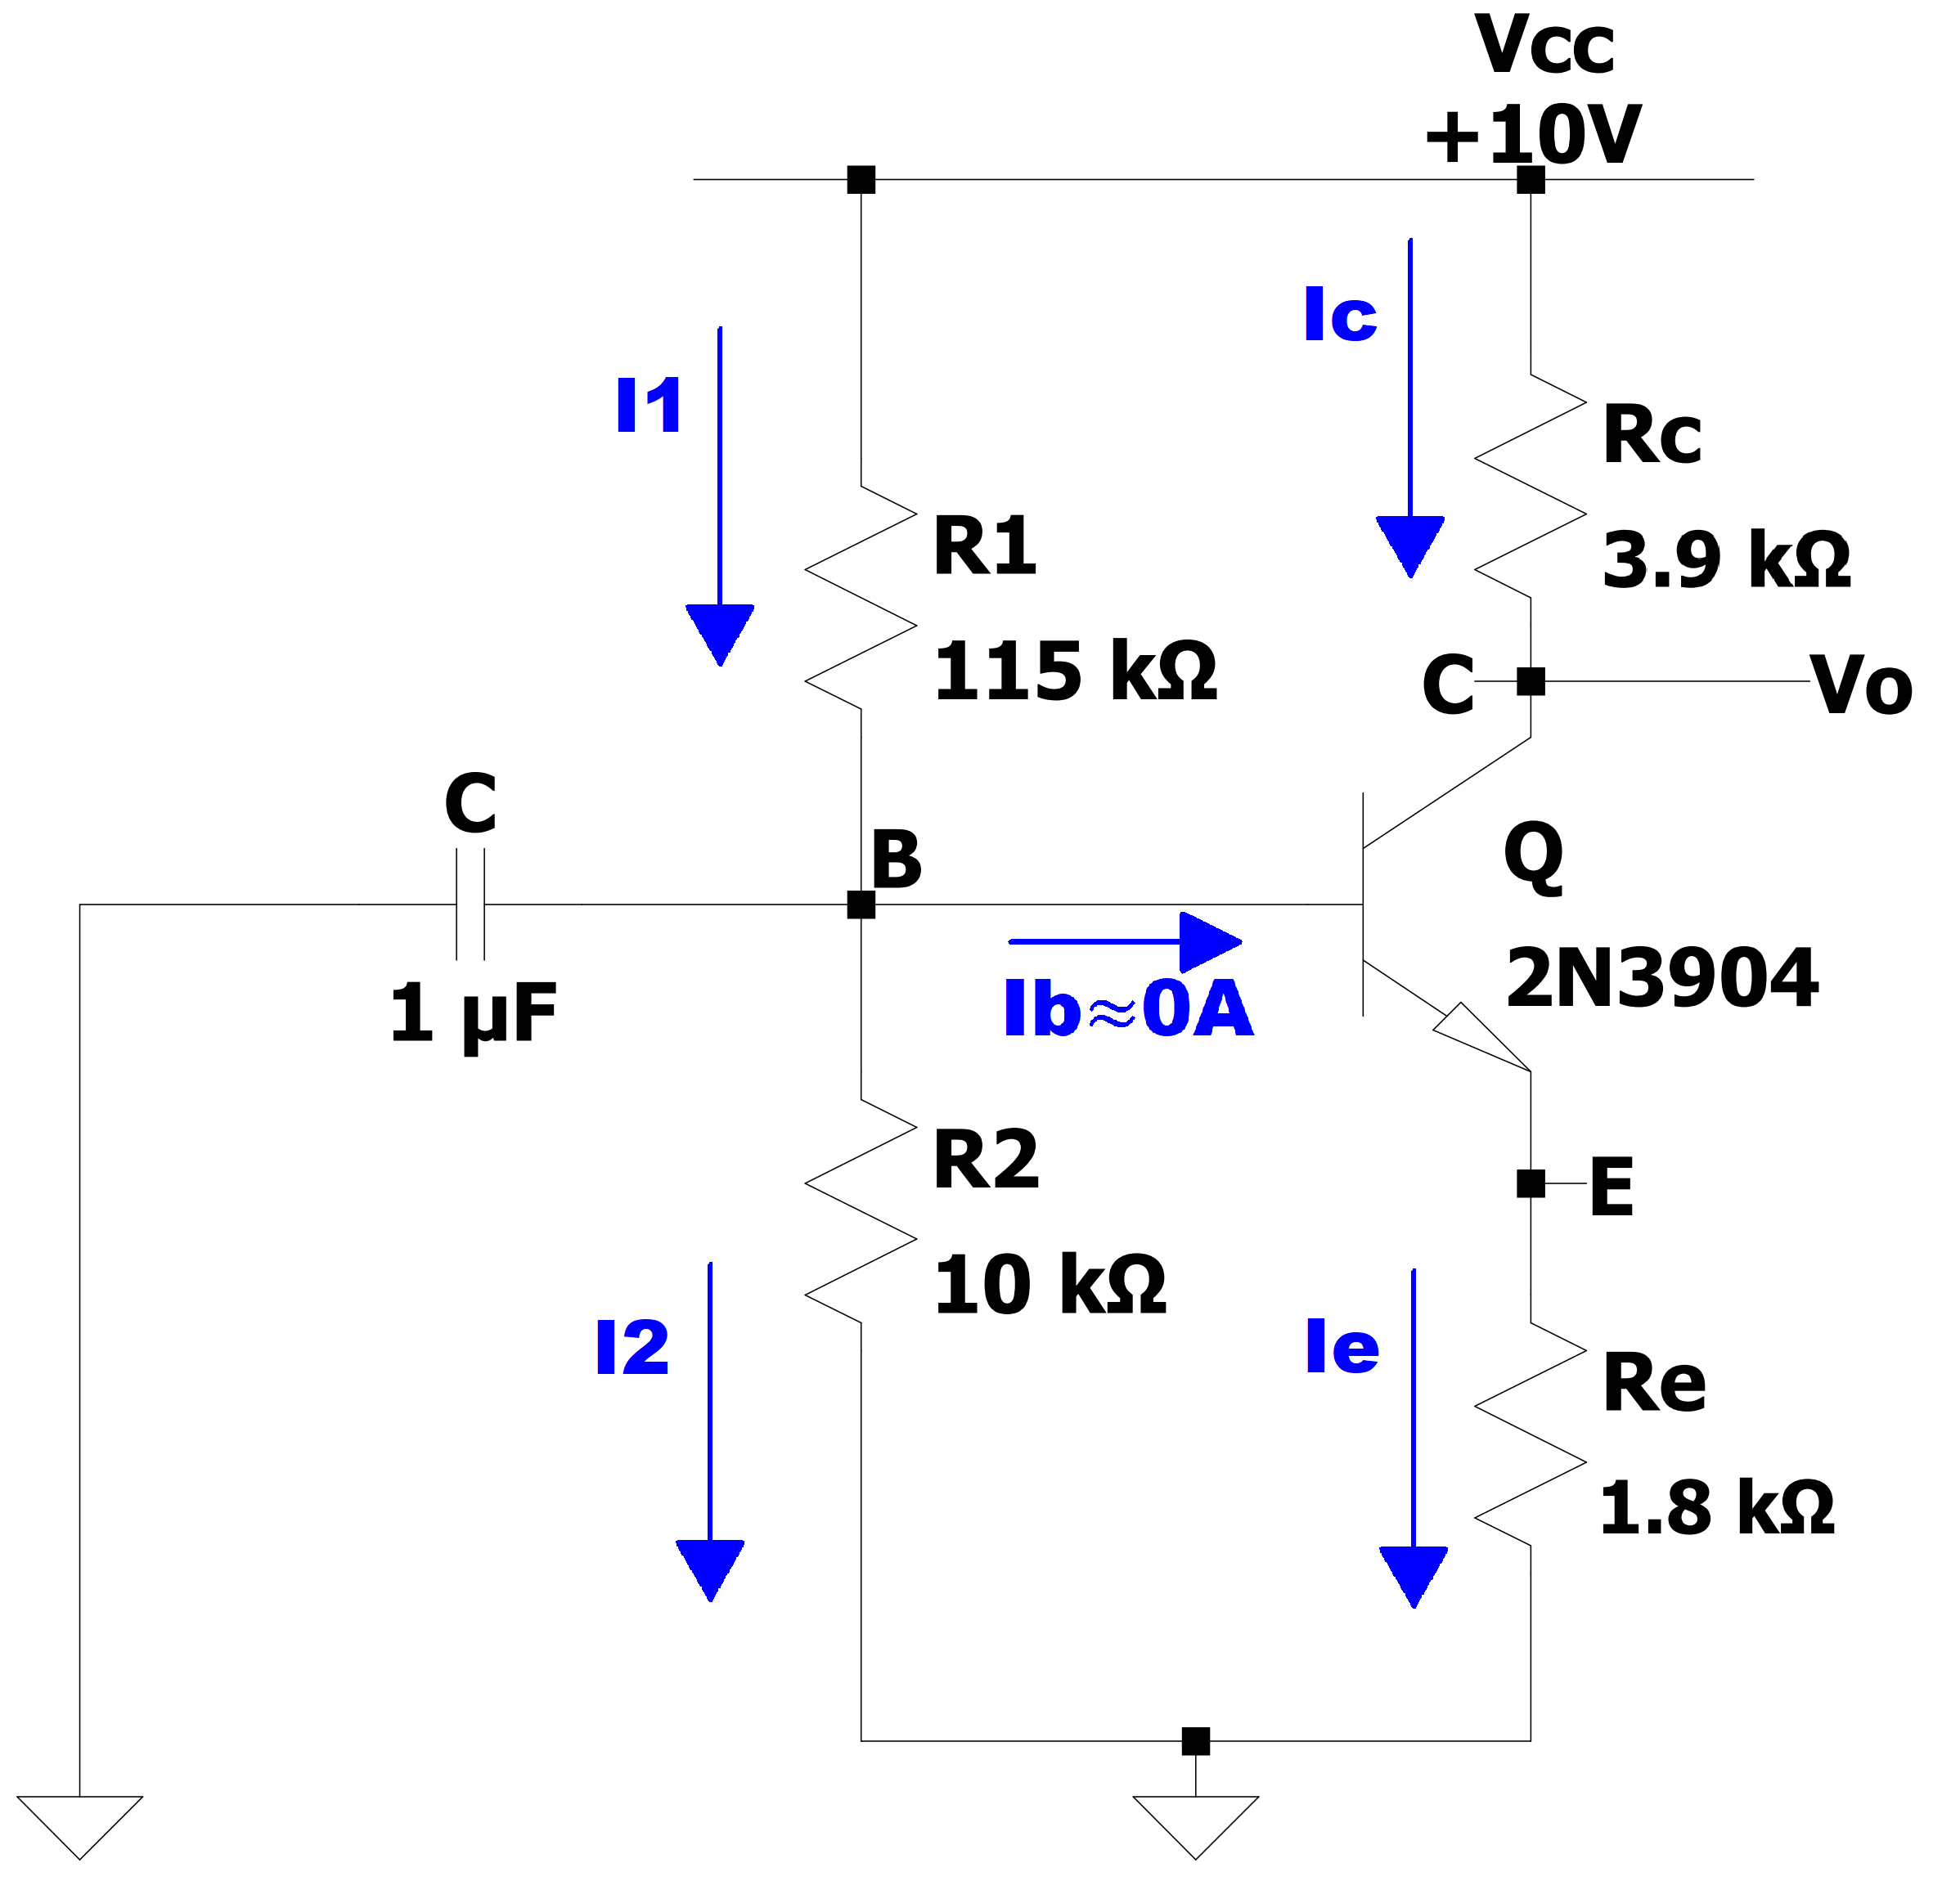
\includegraphics[height=11cm]{immagini/CEv3_pl}
\caption{Punti di lavoro del \textit{Common Emitter amplifier} con degenerazione di emettitore ad alimentazione singola.}
\label{figura:CEv3_pl}
\end{figure}
\\Per l'analisi, assumiamo ancora che $\displaystyle{\beta\rightarrow\infty}$ e che $I_{B}=0A$. La tensione $V_B$ si può ricavare sfruttando il partitore di tensione: %aggiorna
\\[2pt]\indent$\displaystyle{V_B=\frac{R_2}{R_1+R_2}\cdot 10V=\frac{\SI{10}{k\ohm}}{\SI{125}{k\ohm}}\cdot 10V=0.8V}$
\\[2pt]Dato che $I_B$ è nulla, applicando la legge di Kirchhoff al nodo B otteniamo che $I_1=I_2$. Possiamo ricavare una delle due correnti con la legge di Ohm, per esempio calcoliamo $I_2$:
\\[2pt]\indent$\displaystyle{I_2=\frac{V_B-0V}{R_2}=\frac{0.8V}{\SI{10}{k\ohm}}=0.08mA}$
\\[2pt]Per determinare $V_C$, $V_E$, $I_C$ e $I_E$ si procede esattamente come è stato fatto per il circuito precedente.
\\[3pt]In tabella \ref{table:CEv3_pl} sono riassunte tutte le grandezze ricavate dal punto di lavoro. 
\begin{table}[h]
	\centering
	\begin{tabular}{|c|c|c|c|c|c|c|c|c|}
		\hline
		\textbf{V\ped{B}[V]} & \textbf{V\ped{C}[V]} & \textbf{V\ped{E}[V]} & \textbf{I\ped{B}[A]} & \textbf{I\ped{E}[mA]} & \textbf{I\ped{C}[mA]} & \textbf{I\ped{1}[mA]} & \textbf{I\ped{2}[mA]} & \textbf{g\ped{m}[A/V]} \\ 
		\hline
		0.8 & 9 & 0.1 & 0 & 0.100 & 0.100 & 0.056 & 0.056 & 0.0038\\ 
		\hline
	\end{tabular}
\caption{Riassunto delle grandezze ricavate dal punto di lavoro del circuito.}
\label{table:CEv3_pl}
\end{table}
\subsection{Analisi di piccolo segnale}  
Dopo il punto di lavoro, passiamo all'analisi per piccolo segnale. Analogamente a quanto fatto per l'\textit{Emitter follower} ad alimentazione singola, sostituiamo l'alimentazione positiva a 10V con la massa, al posto del transistor utilizziamo il suo modello per piccolo segnale a bassa frequenza ed il condensatore, per ora, non lo sostituiamo con un cortocircuito. Lo schema diventa pertanto quello mostrato in figura \ref{figura:CEv3_ps}.
\begin{figure}[h]
\centering
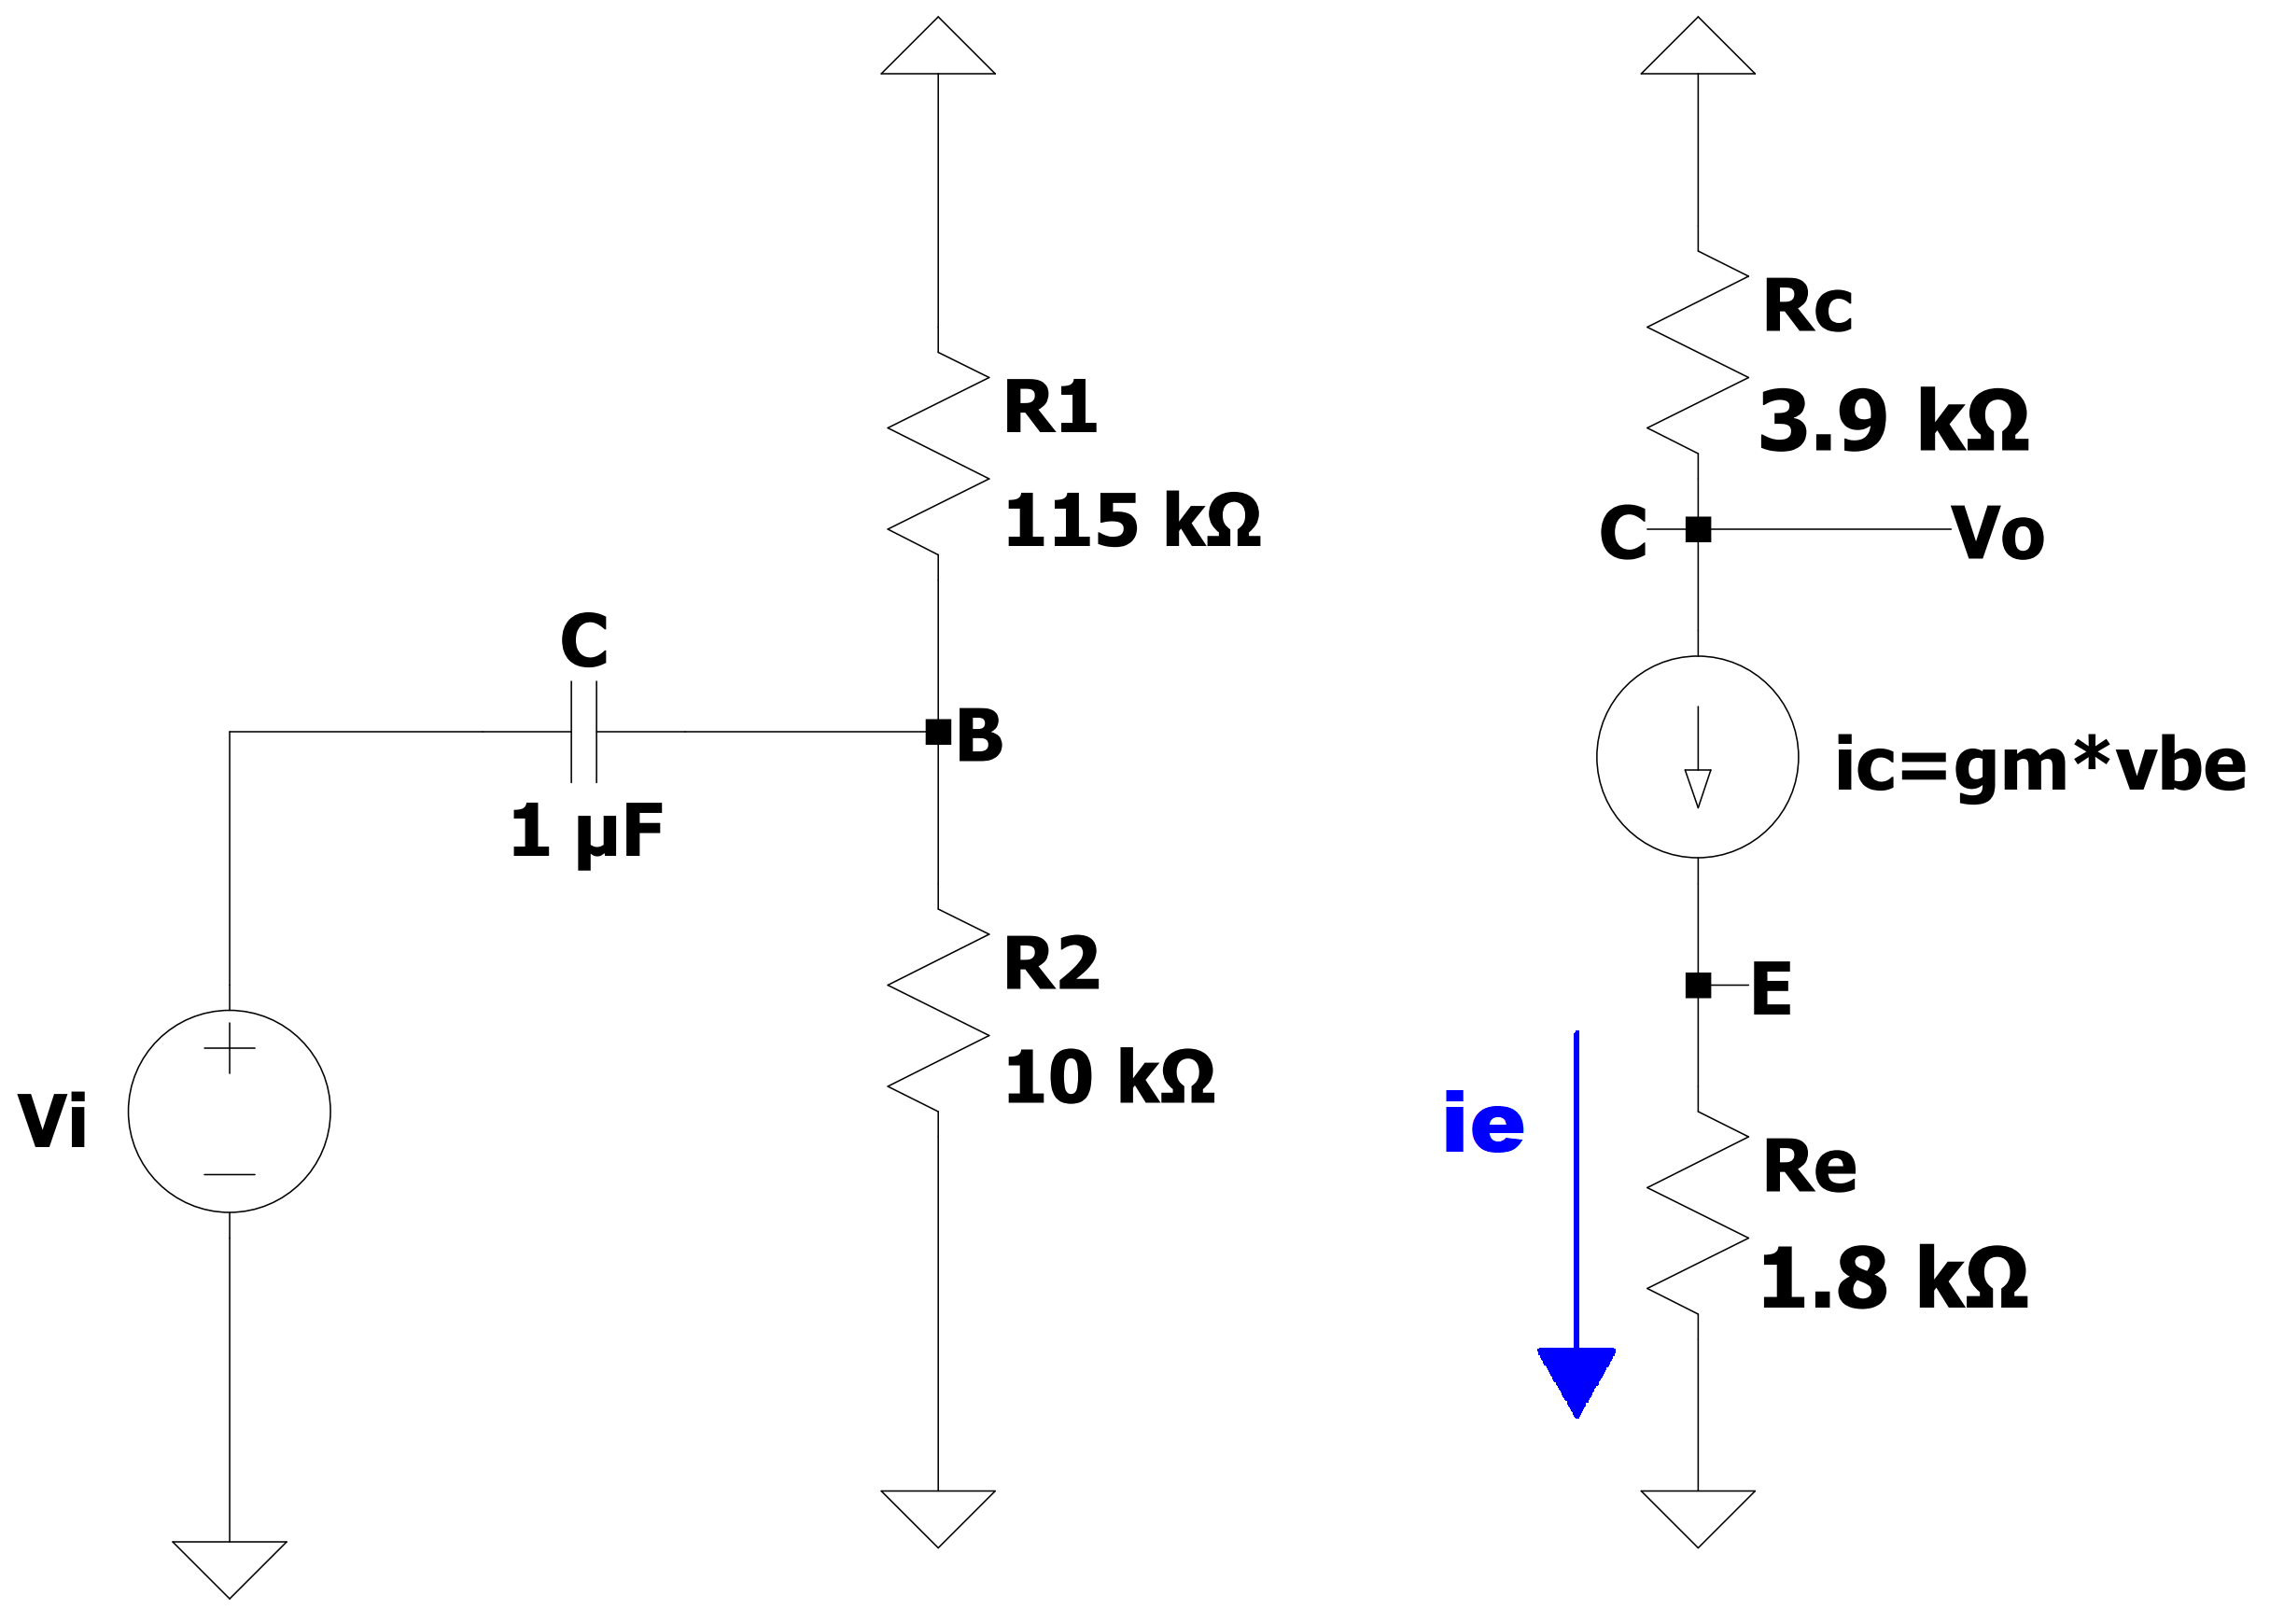
\includegraphics[height=10cm]{immagini/CEv3_ps}
\caption{Schema per l'analisi di piccolo segnale del circuito.}
\label{figura:CEv3_ps}
\end{figure}
\\Il circuito di destra lo risolviamo esattamente come abbiamo fatto per il \textit{Common Emitter amplifier} ad alimentazione duale e discusso nella sezione \ref{CEv3_pscap}, perciò otteniamo la stessa funzione di trasferimento. Si ricorda che questa era pari a:
\\[2pt]\indent $\displaystyle{\frac{v_o}{v_i}=-\frac{g_mR_C}{1+g_mR_E}\simeq -\frac{R_C}{R_E}}$ per $g_mR_E\gg 1$
\\[2pt]Consideriamo invece il circuito di sinistra. Come avveniva per l'\textit{Emitter follower} ad alimentazione singola, il segnale applicato in ingresso entra in un filtro passa-alto. La sua frequenza di taglio, $f_T$ è di:
\\[2pt]\indent $\displaystyle{f_T=\frac{1}{2\pi\cdot C\cdot (R_1\parallelsum R_2)}=\frac{1}{2\pi\cdot 1\mu F\cdot(\SI{115}{k\ohm}\parallelsum\SI{10}{k\ohm})}=\SI{17.30}{\hertz}}$
\\[2pt]Nella sezione \ref{CEv3_miscap} vedremo che se lavoriamo a frequenza sufficientemente elevata ($f\gg f_T$) il contributo del filtro è trascurabile; al contrario, se $f$ è confrontabile con $f_T$ questo non è possibile, perché l'attenuazione data dal filtro modifica notevolmente il segnale che ci aspetteremmo in uscita. 
\subsection{Componenti, strumenti e misure} \label{CEv3_miscap}
Il circuito, di cui si riporta la fotografia (figura \ref{figura:fotoCEv3}), è stato realizzato su una breadboard utilizzando questi componenti:
\begin{itemize}
\item transistor bipolare NPN 2N3904;
\item una resistenza da \SI{3.9}{k\ohm} per $R_C$;
\item una resistenza da \SI{1.8}{k\ohm} per $R_E$;
\item due resistenze, una da \SI{82}{k\ohm} ($R_{11}$) ed una da \SI{27}{k\ohm} ($R_{12}$) connesse in serie, per realizzare la resistenza $R_1$ da \SI{109}{k\ohm};
\item una resistenza da \SI{12}{k\ohm} per $R_2$;
\item un condensatore da \SI{1}{\mu\farad}.
\end{itemize}
Per quanto riguarda $R_1$ ed $R_2$, non è stato possibile utilizzare una resistenza del valore indicato: con questi componenti otteniamo un fattore di partizione di 0.099, contro un valore teorico di 0.08. Perciò, le grandezze del punto di lavoro che misureremo saranno un po' diverse rispetto a quanto calcolato nella sezione \ref{CEv3_plcap}.
\begin{figure}[h]
\centering
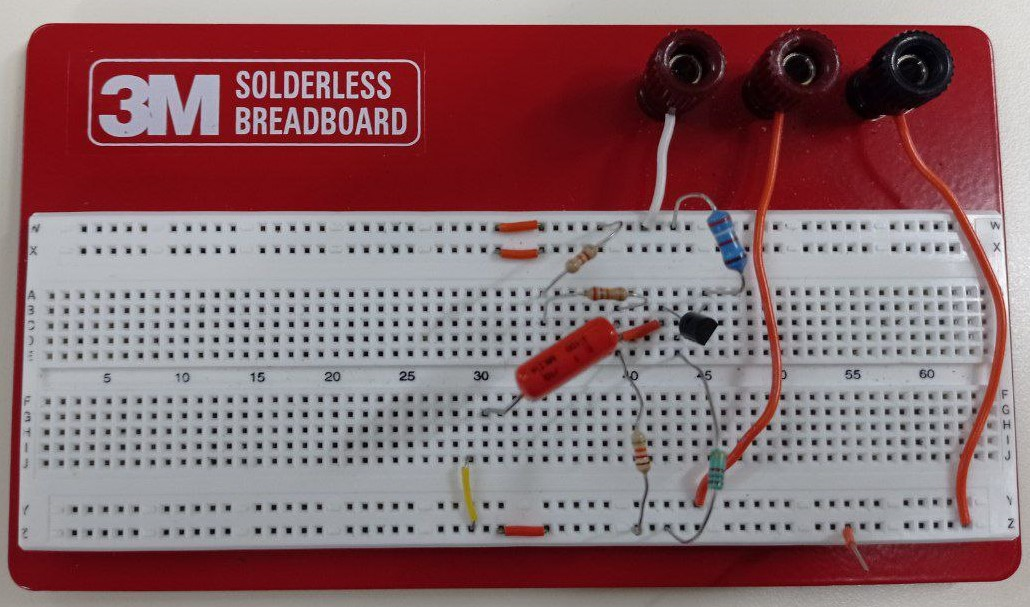
\includegraphics[height=7.8cm]{immagini/fotoCEv3}
\caption{\textit{Common Emitter amplifier} ad alimentazione singola realizzato in laboratorio.}
\label{figura:fotoCEv3}
\end{figure}
\\Per le misure e le analisi, sono stati utilizzati i seguenti strumenti:
\begin{itemize}
\item alimentatore da banco, con alimentazione positiva impostata a 10V e limite in corrente di 50mA;
\item generatore di forme d'onda;
\item multimetro da banco;
\item oscilloscopio a due canali.
\end{itemize}
Come per gli altri circuiti, per prima cosa andiamo a misurare con il multimetro il valore delle resistenze ed i valori delle tensioni delle giunzioni p-n del transistor. I valori ottenuti sono mostrati in tabella \ref{table:CEv3_comp}.
\\
\begin{table}[h]
	\centering
	\begin{tabular}{|c|c|c|}
	\cline{2-3} 
	\multicolumn{1}{c|}{} & \textbf{Valore nominale} & \textbf{Valore misurato}\\ 
		%\hline
		%{} & \textbf{Valore nominale} & \textbf{Valore misurato} \\ 
		\hline
		$\mathbf{R_{C}}$& \SI{3.9}{k\ohm} & \SI{3.907}{k\ohm} \\ 
		\hline
		$\mathbf{R_{E}}$& \SI{1.8}{k\ohm} & \SI{1.807}{k\ohm} \\ 
		\hline
		$\mathbf{R_{11}}$& \SI{82}{k\ohm} & \SI{82.138}{k\ohm} \\ 
		\hline
		$\mathbf{R_{12}}$& \SI{27}{k\ohm} & \SI{26.862}{k\ohm} \\ 
		\hline
		$\mathbf{R_{2}}$& \SI{12}{k\ohm} & \SI{11.953}{k\ohm} \\ 
		\hline
		$\mathbf{V_{BE}}$& $\mathrm{ \simeq0.7V}$ & 0.699V \\ 
		\hline
		$\mathbf{V_{BC}}$& $\mathrm{ \simeq0.7V}$  & 0.659V \\ 
		\hline
	\end{tabular}
\caption{Grandezze misurate prima di realizzare il circuito.}
\label{table:CEv3_comp}
\end{table}
\\Il valore della resistenza $R_1$ sarà quindi pari a \SI{109.000}{k\ohm}. Ora studiamo il punto di lavoro del circuito. Misuriamo le tensioni dei nodi B,C ed E con il multimetro e calcoliamo le correnti $I_1$, $I_2$, $I_C$ e $I_E$ con la legge di Ohm. Ricaviamo quindi per differenza, applicando la legge di Kirchhoff, la corrente $I_B$:
\\[2pt]\indent $\displaystyle{I_1=I_B+I_2\rightarrow I_B=I_1-I_2}$
\\[2pt]Facendo un bilancio di correnti sul transistor otteniamo:
\\[2pt]\indent $\displaystyle{I_E=I_C+I_B}$
\\[2pt]Questa equazione può essere utilizzata per verificare che le correnti calcolate siano corrette.
\\Tutti i valori misurati o calcolati sono riportati in tabella \ref{table:EFv2_3_pl_mis}. 
%% DA QUI
\begin{table}[h]
	\centering
	\begin{tabular}{|c|c|c|c|c|c|c|c|c|}
		\hline
		\textbf{V\ped{B}[V]} & \textbf{V\ped{C}[V]} & \textbf{V\ped{E}[V]} & \textbf{I\ped{1}[mA]} & \textbf{I\ped{2}[mA]} & \textbf{I\ped{B}[mA]} & \textbf{I\ped{E}[mA]} & \textbf{I\ped{C}[mA]} & \textbf{g\ped{m}[A/V]} \\ 
		\hline
		0.973 & 9.238 & 0.354 & 0.083 & 0.081 & 0.002 & 0.196 & 0.195 & 0.075\\ 
		\hline
	\end{tabular}
\caption{Grandezze misurate dallo studio del punto di lavoro del circuito.}
\label{table:EFv2_3_pl_mis}
\end{table}
\\I valori ottenuti sono leggermente maggiori di quelli che abbiamo calcolato nell'analisi teorica, ma questo non deve stupirci perché il fattore di partizione del circuito realizzato è maggiore di quello teorico. Il bilancio di correnti sul transistor è: $I_B+I_C=0.002mA+0.195mA=0.197mA$, che risulta corretto dato che commentiamo un errore dell'ordine del \textmu A.
\\\indent Dopo lo studio del punto di lavoro, con il generatore di forme d'onda applichiamo in ingresso al circuito delle sinusoidi. Collegando al circuito le sonde dell'oscilloscopio, osserviamo il grafico della tensione in ingresso e della tensione in uscita. La prima forma d'onda utilizzata è una sinusoide di frequenza $f=\SI{1}{k\hertz}$ e tensione picco-picco $V_{PP}$ di 100mV. Il grafico è riportato in figura \ref{figura:oscillo6}, i due segnali sono accoppiati in AC.
\begin{figure}[h]
\centering
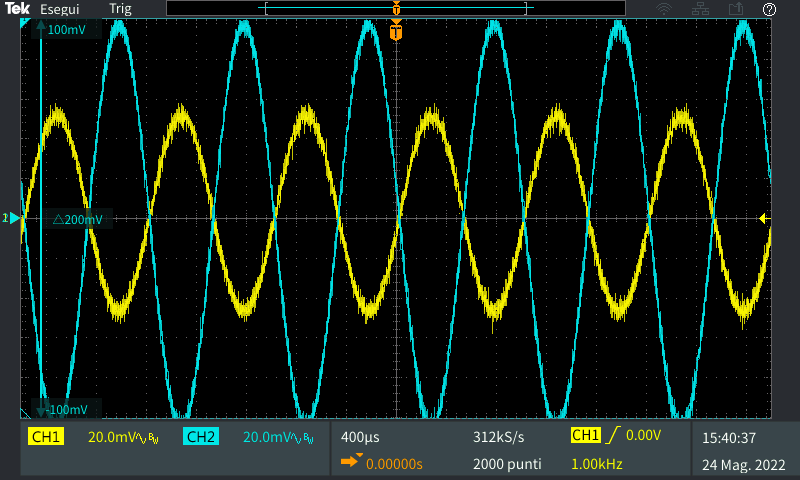
\includegraphics[height=7.5cm]{immagini/oscillo6}
\caption{Grafico della tensione in ingresso (CH1) e della tensione in uscita (CH2) al circuito.}
\label{figura:oscillo6}
\end{figure}
\\Dato che l'ampiezza della sinusoide è piuttosto piccola, i segnali non risultano molto ``puliti'' a causa del rumore elettronico. Il rumore elettronico non è eliminabile, ma dato che è una grandezza statistica a media 0, possiamo sfruttare l'oscilloscopio per mediare su 64 campioni l'ingresso e l'uscita, in questo modo otteniamo dei segnali molto più puliti. Questo grafico è mostrato in figura \ref{figura:oscillo7}, i segnali sono ancora accoppiati in AC.  
\begin{figure}[h]
\centering
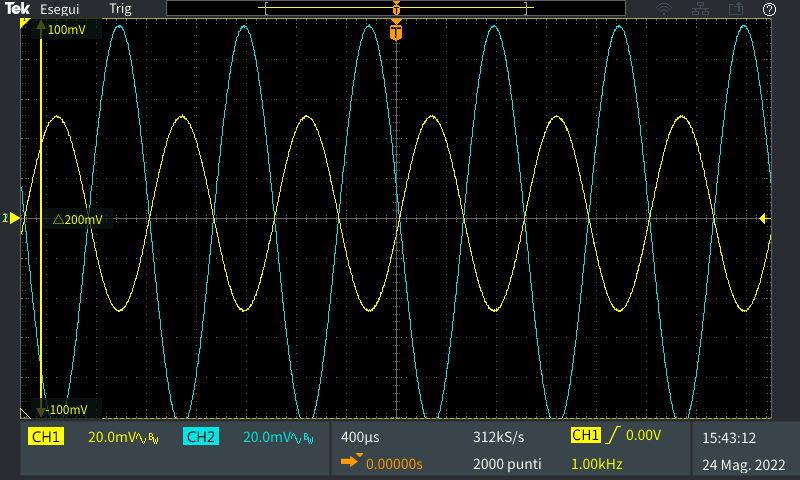
\includegraphics[height=7.2cm]{immagini/oscillo7}
\caption{Grafico delle tensioni precedenti mediate su 64 campioni.}
\label{figura:oscillo7}
\end{figure}
\\Proviamo ora ad applicare un'altra sinusoide, sempre alla stessa frequenza ma con tensione picco-picco $V_{PP}$ di 1V. L'uscita è prelevata dal collettore, la sua tensione DC l'abbiamo già misurata e sappiamo che è pari a 9.238V. Dato che la tensione picco-picco è di 1V, il valore maggiore che la sinusoide può raggiungere è di 500mV. Il guadagno del circuito è di 2.17, perciò l'ampiezza massima che la sinusoide in uscita può raggiungere è di 1.085V. Se sommiamo alla componente continua dell'uscita il massimo valore della componente alternata dell'uscita, otteniamo un valore di tensione di 10.323V. Però il circuito è alimentato fra massa e 10V, quindi non può fornire in uscita una tensione maggiore di 10V: con questo ingresso, l'uscita satura, dunque il tratto di semionda che dovrebbe essere maggiore di 10V, in realtà sarà costante e pari al valore della tensione di alimentazione. Il grafico è illustrato in figura \ref{figura:oscillo8}.
\begin{figure}[h]
\centering
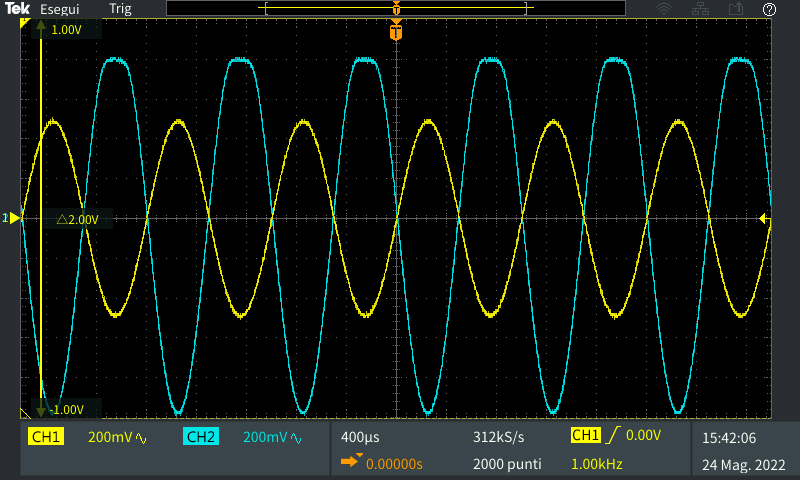
\includegraphics[height=7.2cm]{immagini/oscillo8}
\caption{Grafico delle due tensioni. Si può notare che l'uscita satura.}
\label{figura:oscillo8}
\end{figure}
\\Se aumentiamo ulteriormente la tensione picco-picco del segnale in ingresso, l'effetto è ancor più visibile. In figura \ref{figura:oscillo9} è stato usato un segnale sinusoidale con $V_{PP}=3$V e $f=\SI{10}{k\hertz}$.
\begin{figure}[h]
\centering
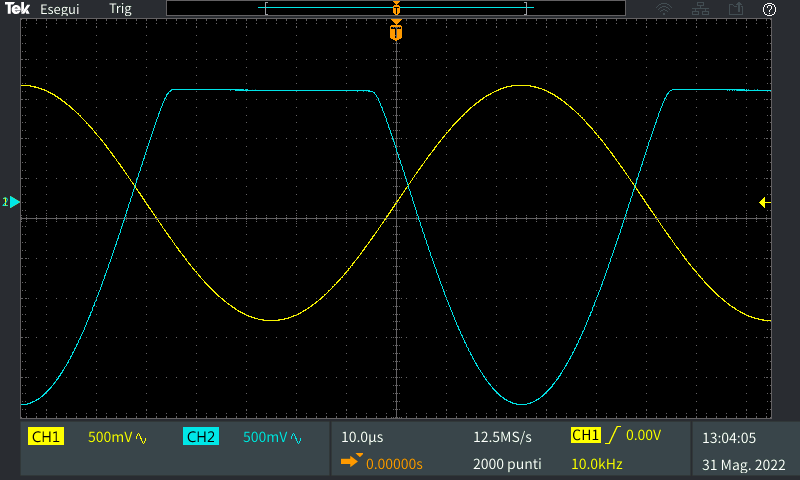
\includegraphics[height=8cm]{immagini/oscillo9}
\caption{Grafico della tensione in uscita quando V\ped{PP}=3V. L'uscita satura.}
\label{figura:oscillo9}
\end{figure}
\\Un altro studio che si può fare su questo circuito riguarda il contributo del filtro passa-alto a diverse frequenze. La funzione di trasferimento del filtro nel dominio di Laplace la si può ricavare tramite un bilancio di correnti al nodo B. La tensione in ingresso è $v_i\left(s\right)$ e la tensione in uscita al filtro è $v_B\left(s\right)$. La funzione di trasferimento del filtro è:
\\[2pt]\indent $\displaystyle{v_B\left(s\right)=\frac{s\left(R_1\parallelsum R_2\right)C}{1+s\left(R_1\parallelsum R_2\right)C}\cdot v_i\left(s\right)}$
\\[2pt]Se passiamo al regime alternato, dobbiamo sostituire $s$ con $j\omega$, pertanto la funzione di trasferimento risulta: 
\\[2pt]\indent $\displaystyle{v_B\left(\omega\right)=\frac{j\omega\left(R_1\parallelsum R_2\right)C}{1+j\omega\left(R_1\parallelsum R_2\right)C}\cdot v_i\left(\omega\right)}$, con $\displaystyle{\omega=2\pi f}$
\\[2pt]Perciò, la tensione della base del transistor, $v_B\left(j\omega\right)$, dipende dalla frequenza alla quale lavoriamo.
\\Il parallelo delle due resistenze $R_1$ e $R_2$ vale:
\\[2pt]\indent $\displaystyle{R_1\parallelsum R_2=R_{eq}=\frac{R_1\cdot R_2}{R_1+R_2}=\frac{\SI{109}{k\ohm}\cdot\SI{12}{k\ohm}}{\SI{109}{k\ohm}+\SI{12}{k\ohm}}=\SI{10.810}{k\ohm}}$
\\[2pt]La frequenza di taglio con i parametri $R_1$, $R_2$ e $C$ del nostro filtro è $f_T=\SI{14.72}{\hertz}$, che corrisponde ad una pulsazione di $\omega_T=\SI{92.49}{\radian/s}$. 
\\\indent Proviamo quindi ad applicare due segnali sinusoidali, entrambi con tensione picco-picco di 100mV, la frequenza del primo segnale è \SI{10}{\hertz}, corrispondente ad una pulsazione di \SI{62.83}{\radian/s}, invece la frequenza del secondo è \SI{10}{k\hertz}, corrispondente ad una pulsazione di \SI{6283.19}{\radian/s}. Ci aspettiamo che con il primo segnale il circuito non funzionerà come un \textit{Common Emitter amplifier}, perché l'effetto del filtro non sarà trascurabile, dato che lavoriamo ad una frequenza minore di quella di taglio; al contrario, con il secondo segnale il circuito dovrebbe funzionare correttamente, dato che siamo ad una frequenza molto maggiore rispetto a quella di taglio.
\\\indent Nei grafici seguenti vediamo la tensione in ingresso e la tensione in uscita quando applichiamo il primo segnale (figura \ref{figura:oscillo10}) e quando invece applichiamo il secondo (\ref{figura:oscillo11}).
\begin{figure}[h]
\centering
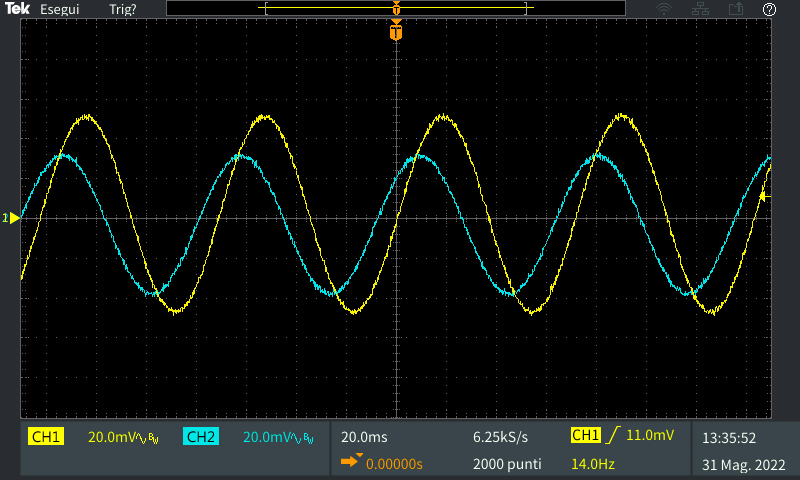
\includegraphics[height=8.4cm]{immagini/oscillo10}
\caption{Grafico della tensione in ingresso e in uscita al circuito con il primo segnale.}
\label{figura:oscillo10}
\end{figure}
\begin{figure}[h!]
\centering
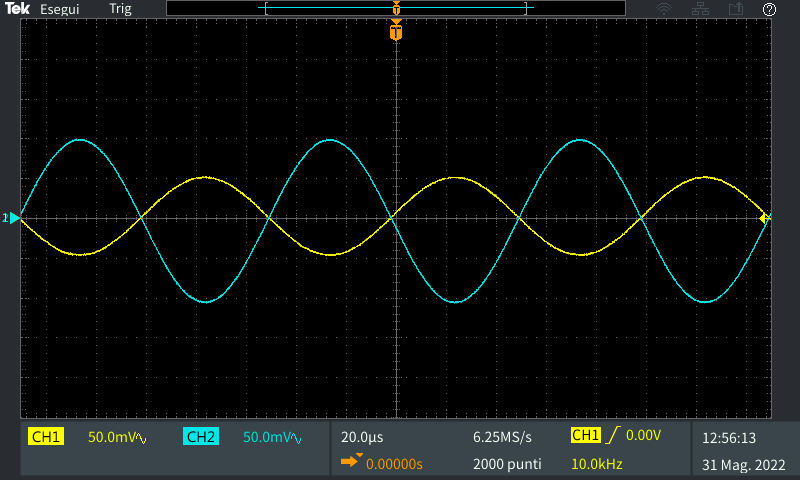
\includegraphics[height=8.4cm]{immagini/oscillo11}
\caption{Grafico della tensione in ingresso e in uscita al circuito con il secondo segnale.}
\label{figura:oscillo11}
\end{figure}
\\Con il secondo segnale il circuito funziona correttamente. Con il primo segnale invece no, in particolare, l'uscita è sia attenuata che sfasata rispetto al segnale in ingresso. Per capire meglio cosa succede, è utile guardare il diagramma di Bode di modulo e fase del filtro passa-alto. Questo è rappresentato nella figura seguente (figura \ref{figura:grafico2}), sono inoltre riportati i valori di modulo e fase in corrispondenza della pulsazione di taglio e delle pulsazioni dei due segnali utilizzati.
\begin{figure}[h]
\centering
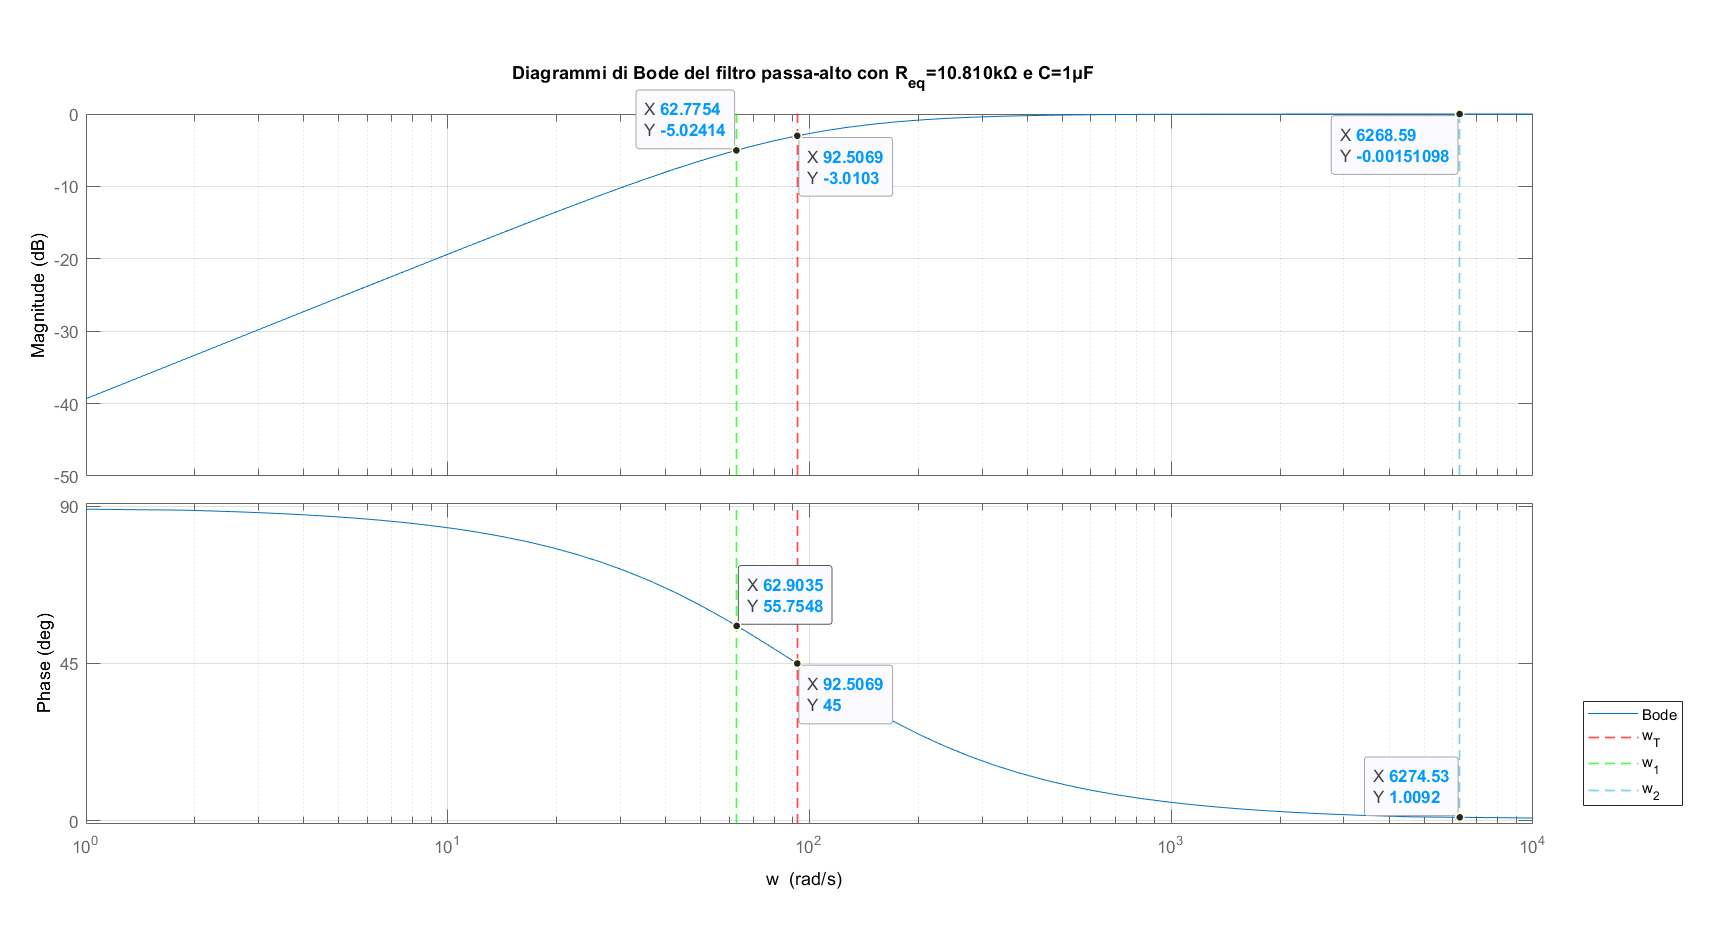
\includegraphics[width=\textwidth]{immagini/graficoCEv3}
\caption{Diagramma di Bode di modulo e fase del filtro passa-alto.}
\label{figura:grafico2}
\end{figure}
\\Dal grafico precedente vediamo che il primo segnale subisce un'attenuazione di -5.0241dB, che in scala decimale corrisponde a 0.5608: la tensione picco-picco del segnale in uscita al filtro è quasi dimezzata, sarà pari a circa 56.080mV. Tuttavia, nello stadio successivo il segnale viene amplificato di un fattore pari al rapporto fra la resistenza di collettore e quella di emettitore, ricordiamo che per il nostro circuito questo fattore vale 2.16. Allora, la tensione picco-picco del segnale in uscita al circuito è circa 121.133mV. Questo risultato non corrisponde perfettamente alla tensione picco-picco misurata in uscita al circuito con l'oscilloscopio (figura \ref{figura:oscillo10}), ma va notato che l'acquisizione con l'oscilloscopio è molto rumorosa, inoltre anche il valore del modulo è approssimativo. Il filtro introduce anche uno sfasamento, che a questa frequenza è circa pari a 55.7548°. Questo contributo va a sommarsi allo sfasamento di 180° dato dallo stadio successivo, ed il valore totale dello sfasamento è confrontabile con il grafico di figura \ref{figura:oscillo10}.
\\\indent Consideriamo ora il secondo segnale: quando questo attraversa il filtro, viene attenuato di circa -0.0015dB, ovvero 0.9998 in scala decimale, e sfasato di 1.0092°. È evidente che dal punto di vista pratico, questi valori non modificano il segnale, perciò il contributo del filtro può tranquillamente essere trascurato quando si analizza il circuito, senza che quest'approssimazione alteri la bontà dei risultati ottenuti.  
%----------------------------------------------------------------------------------------
%	CIRCUITI 3 E 4: AMPLIFICATORE OPERAZIONALE \mu A741
%----------------------------------------------------------------------------------------
\clearpage
\newpage
\chapter{Circuiti 3 e 4: Amplificatore operazionale \textmu A741}
\section{Introduzione} 
I due circuiti discussi di seguito sono stati realizzati utilizzando un amplificatore operazionale \textit{general purpose}, il \textmu A741. Per primo abbiamo realizzato un amplificatore invertente (sezione \ref{amplinv_cap}), poi, aggiungendo un condensatore al circuito precedente, abbiamo ottenuto un integratore (sezione \ref{int_cap}). Nell'immagine sottostante, la figura \ref{figura:741}, si possono vedere i numeri e la funzione di ogni terminale. Per i nostri circuiti, connettermo i terminali in questo modo:
\begin{itemize}
\item il terminale numero 8 è \textit{Not Connected}, perciò non viene collegato a nulla;
\item i terminali 7 e 4 sono collegati rispettivamente all'alimentazione positiva e all'alimentazione negativa;
\item i terminali 1 e 5 servono per compensare l'offset, li lasceremo floating (in generale è una cosa che non andrebbe fatta, perché non abbiamo modo di sapere a che tensione si troveranno);
\item il terminale 3, ovvero l'ingresso non-invertente, lo connettiamo a massa;
\item il terminale 2 è l'ingresso invertente. A questo terminale applicheremo, anche se non direttamente, il segnale; 
\item il terminale 6 serve per prelevare l'output.
\end{itemize}
\begin{figure}[h]
\centering
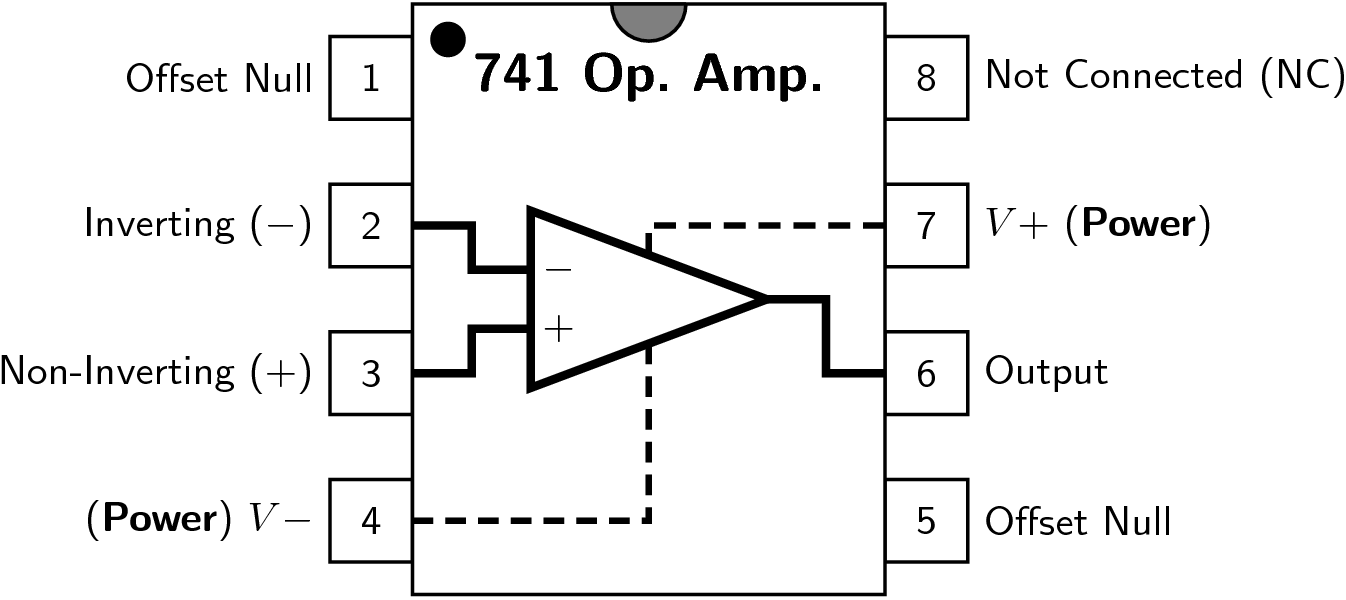
\includegraphics[height=5.5cm]{immagini/741pinout}
\caption{Package e funzione dei pin del \textmu A741.}
\label{figura:741}
\end{figure}
\section{Amplificatore invertente} \label{amplinv_cap} 
Il primo circuito realizzato utilizzando il \textmu A741 è l'amplificatore invertente. Di seguito si riportano lo schema, l'analisi del circuito e le misure effettuate su di questo.
\subsection{Schema} 
\begin{figure}[h]
\centering
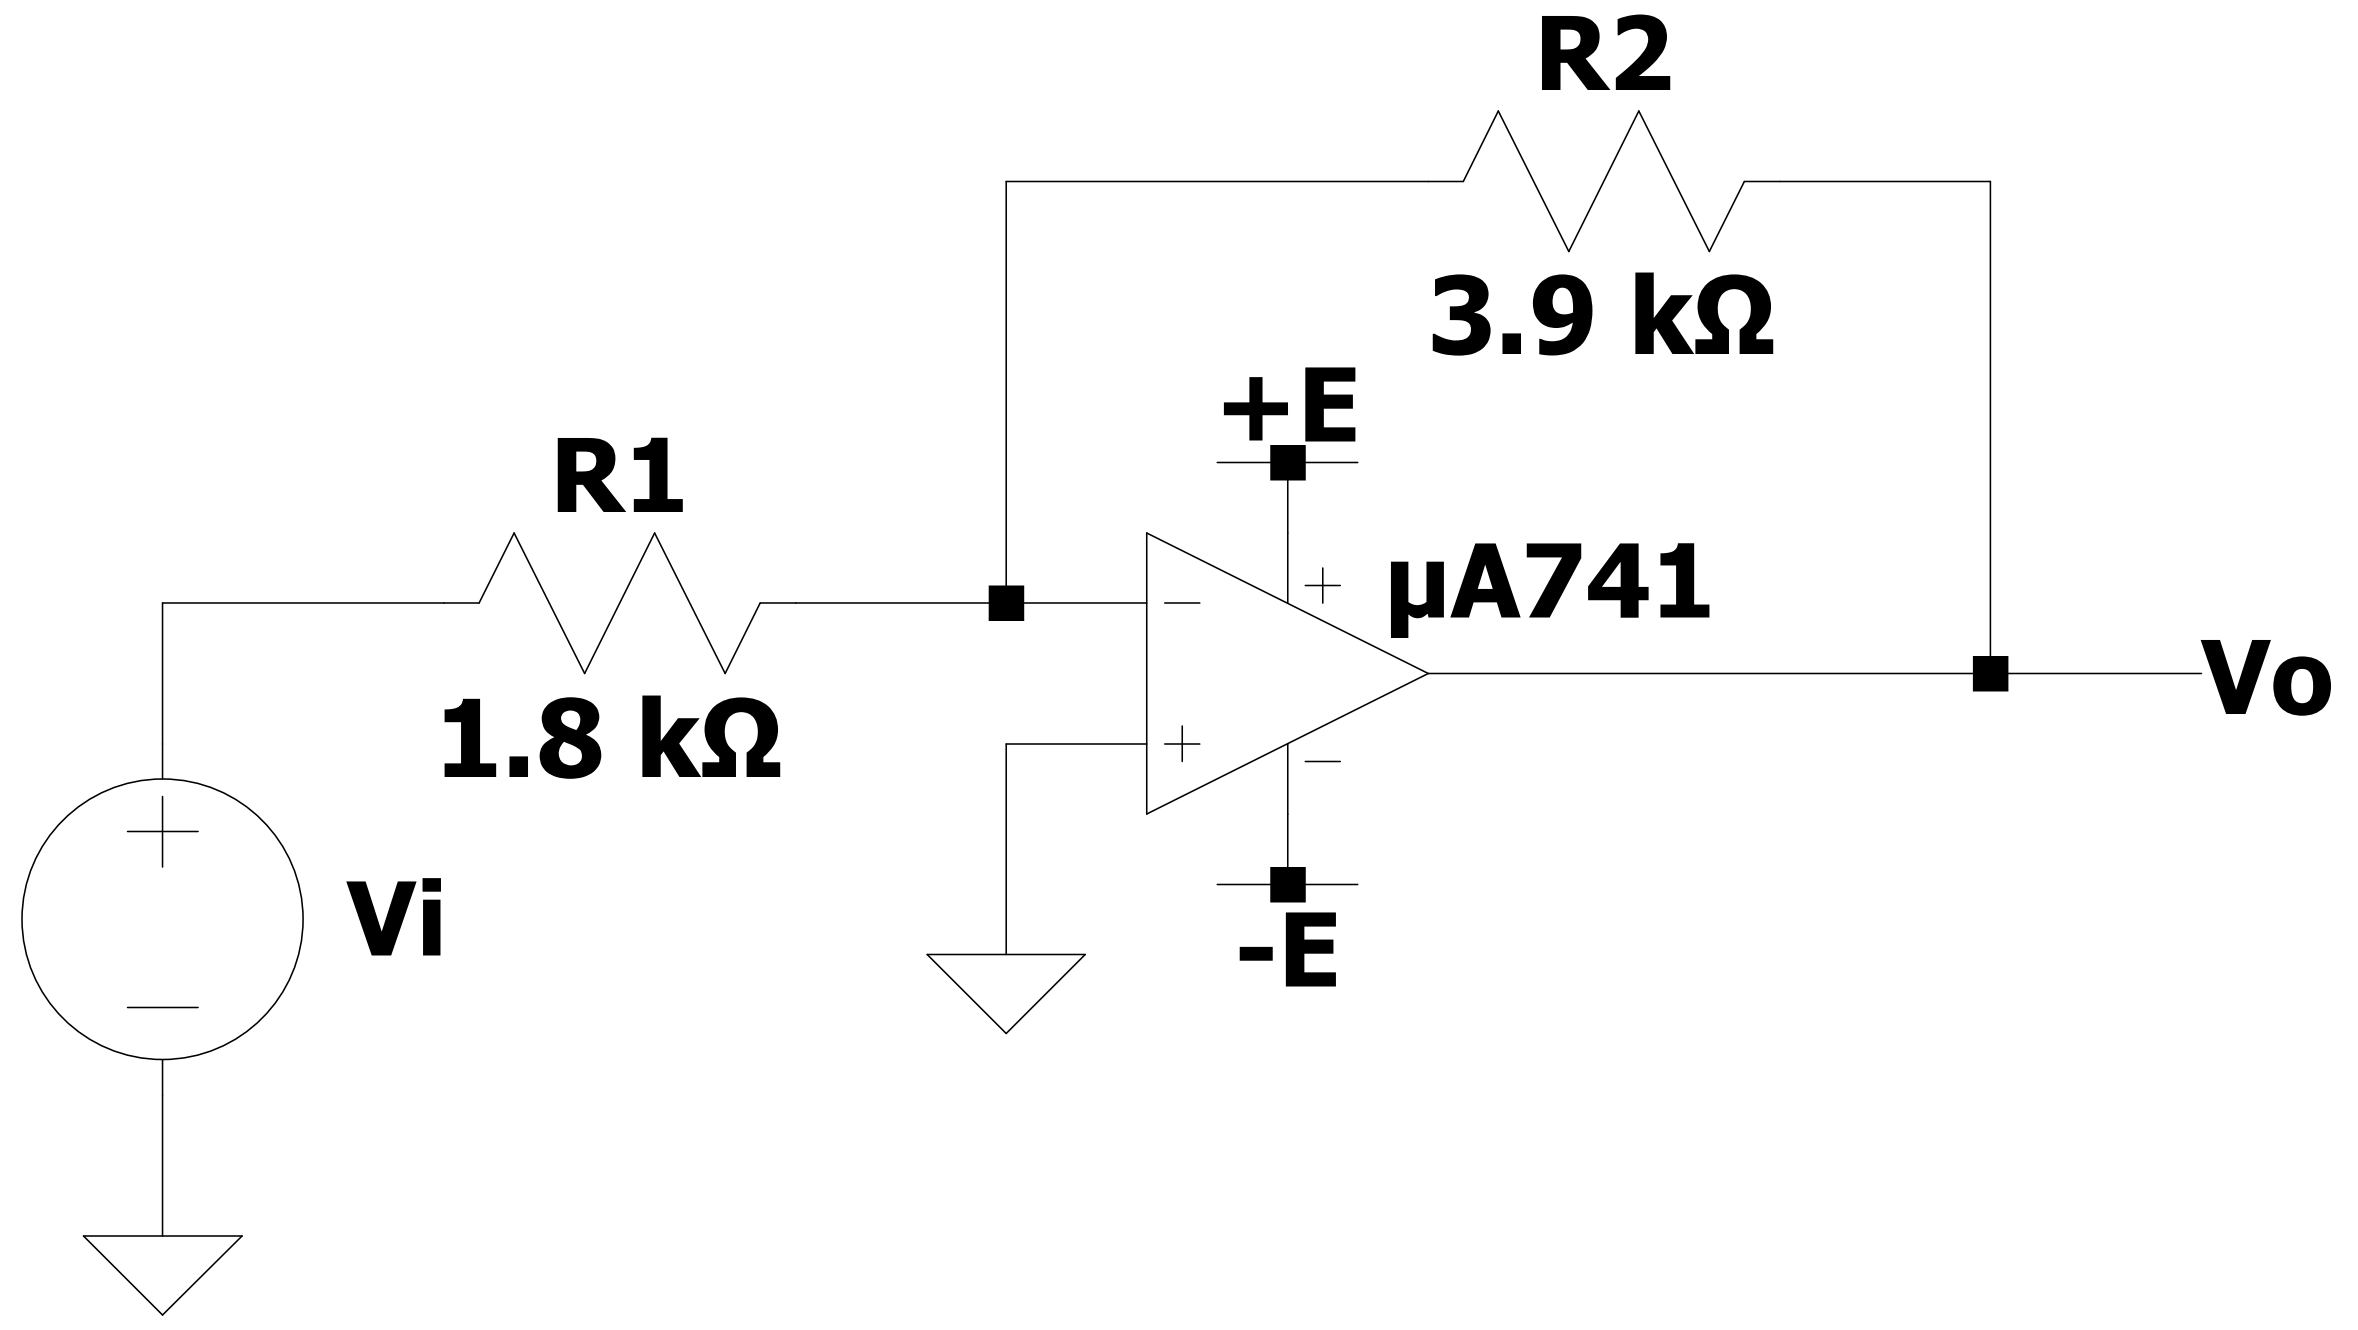
\includegraphics[height=7.5cm]{immagini/amplinv}
\caption{Schema dell'amplificatore invertente.}
\label{figura:amplinv}
\end{figure}
\subsection{Analisi del circuito} \label{amplinv_analisi_cap}
Il circuito è retroazionato negativamente, perché l'uscita viene riportata all'ingresso invertente dell'amplificatore operazionale. Per ricavare la funzione di trasferimento del circuito è sufficiente fare un bilancio di correnti all'ingresso invertente:
\\[2pt]\indent $I_1=I_2+I_{in^-}$
\\[2pt]La corrente in ingresso all'OPAMP è molto piccola, idealmente $I_{in^+}=I_{in^-}\rightarrow 0A$. Perciò l'equazione precedente diventa:
\\\indent $\displaystyle{I_1=I_2}$
\\Utilizzando la legge di Ohm, le due correnti si possono esprimere come:
\\[2pt]\indent $\displaystyle{\frac{V^--V_i}{R_1}=\frac{V_o-V^-}{R2}}$
\\[2pt]Se un circuito è retroazionato negativamente, $V^+=V^-$ per il principio del cortocircuito virtuale. Dato che $V^+$ è a massa, la sua tensione è di 0V, di conseguenza anche $V^-$ si troverà a questa tensione. L'equzione precedente diventa:
\\[2pt]\indent $\displaystyle{\frac{-V_i}{R_1}=\frac{V_o}{R2}}$
\\[2pt]Tramite quest'equazione è facile ricavare la funzione di trasferimento del circuito, che risulta:
\\[2pt]\indent $\displaystyle{\frac{V_o}{V_i}=-\frac{R_2}{R_1}}$
\\[2pt]Come suggerisce il nome del circuito, è un amplificatore perché se $R_2>R_1$ il segnale in ingresso viene amplificato. È inoltre invertente, perché compare un segno meno nella funzione di trasferimento, pertanto ingresso e uscita saranno in controfase (sfasate di 180°).
\\Per il nostro circuito la resistenza $R_1$ è di \SI{1.8}{k\ohm} e la resistenza $R_2$ è di \SI{3.9}{k\ohm}, perciò il guadagno, in modulo, vale 2.17.
\subsection{Componenti, strumenti e misure} 
Il circuito è stato realizzato su una breadboard utilizzando questi componenti:
\begin{itemize}
\item una resistenza da \SI{3.9}{k\ohm} per $R_2$;
\item una resistenza da \SI{1.8}{k\ohm} per $R_1$;
\item amplificatore operazionale \textmu A741.
\end{itemize}
Per le misure e le analisi, sono stati utilizzati i seguenti strumenti:
\begin{itemize}
\item alimentatore da banco, con alimentazione positiva impostata a 5V ed alimentazione negativa a -5V, entrambe con limite in corrente di 50mA;
\item generatore di forme d'onda;
\item multimetro da banco;
\item oscilloscopio a due canali.
\end{itemize}
In figura \ref{figura:foto_amplinv} è mostrata una fotografia del circuito in cui possiamo vedere dove applichiamo il segnale. Nella fotografia, il pin numero 1 del \textmu A741 si trova in basso a sinistra.
\begin{figure}[h]
\centering
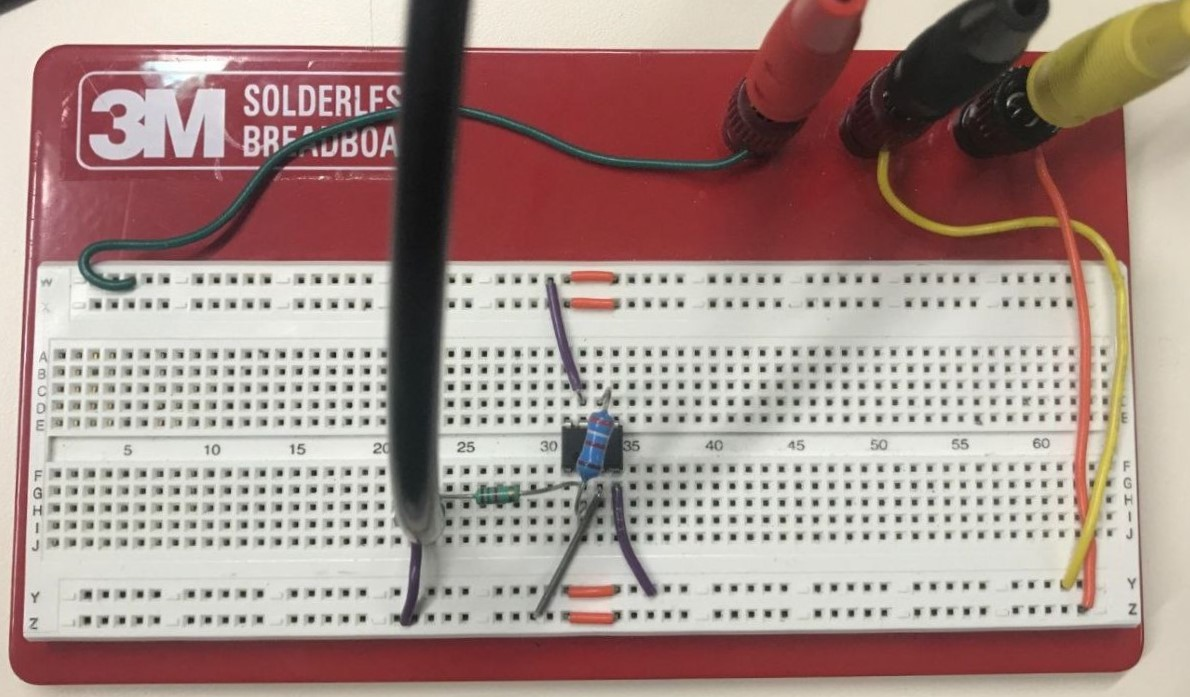
\includegraphics[height=9cm]{immagini/foto_amplinv}
\caption{Amplificatore invertente con \textmu A741.}
\label{figura:foto_amplinv}
\end{figure}
\\Per prima cosa, con il multimetro si sono misurati i valori delle resistenze. I valori ottenuti sono mostrati in tabella \ref{table:amplinv_comp}.
\begin{table}[h]
	\centering
	\begin{tabular}{|c|c|c|}
	\cline{2-3} 
	\multicolumn{1}{c|}{} & \textbf{Valore nominale} & \textbf{Valore misurato}\\ 
		%\hline
		%{} & \textbf{Valore nominale} & \textbf{Valore misurato} \\ 
		\hline
		$\mathbf{R_1}$& \SI{1.8}{k\ohm} & \SI{1.807}{k\ohm} \\ 
		\hline
		$\mathbf{R_2}$& \SI{3.9}{k\ohm} & \SI{3.907}{k\ohm} \\ 
		\hline
	\end{tabular}
\caption{Grandezze misurate prima di realizzare il circuito.}
\label{table:amplinv_comp}
\end{table}
\\Dopo aver posizionato tutti i componenti sulla breadboard, è stato applicato il segnale, successivamente abbiamo collegato le sonde dell'oscilloscopio. La sonda del canale 1 è stata collegata al terminale della resistenza $R_1$ non collegato al pin 2 del \textmu A741; la sonda del canale 2 è invece stata collegata al terminale della resistenza $R_2$ connesso con il pin 6 dell'OPAMP. Con il primo canale visualizziamo la tensione in ingresso, mentre con il secondo la tensione in uscita al circuito. 
\\\indent Dal rapporto fra le resistenze misurate, ci aspettiamo un guadagno di 2.16. Sono state applicate due sinusoidi, entrambe di frequenza \SI{1}{k\hertz}, ma con diversa tensione picco-picco: il primo segnale ha una $V_{PP}$ di 1V, il grafico è la figura \ref{figura:oscillo12}, il secondo segnale ha invece una $V_{PP}$ di 2V, il grafico è la figura \ref{figura:oscillo13}.
\begin{figure}[h]
\centering
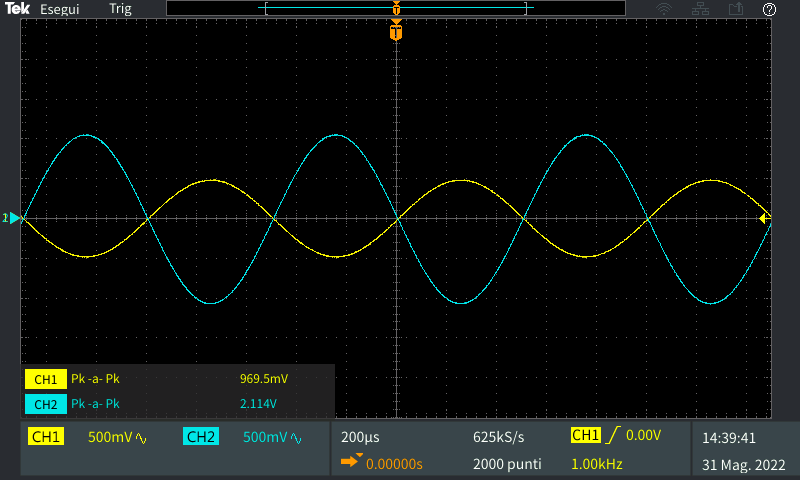
\includegraphics[height=9cm]{immagini/oscillo12}
\caption{Grafico della tensione in ingresso e in uscita al circuito con il primo segnale.}
\label{figura:oscillo12}
\end{figure}
\begin{figure}[h]
\centering
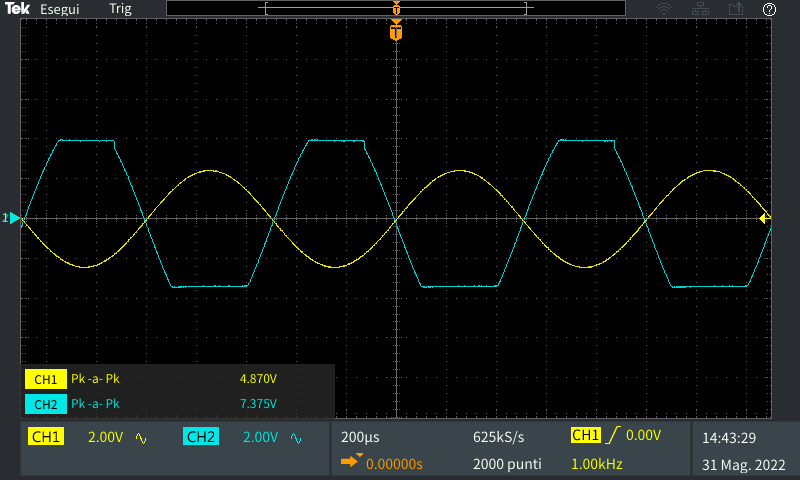
\includegraphics[height=8.9cm]{immagini/oscillo13}
\caption{Grafico della tensione in ingresso e in uscita al circuito con il secondo segnale.}
\label{figura:oscillo13}
\end{figure}
\\Per quanto riguarda il primo segnale, se facciamo il rapporto fra la misura della tensione picco-picco del segnale in ingresso e la misura della tensione picco-picco del segnale in uscita otteniamo un valore di 2.18, che è vicinissimo al guadagno che dobbiamo ottenere dal circuito.
\\\indent Con il secondo segnale, invece, l'uscita satura. Infatti, l'uscita un amplificatore operazionale ideale non può mai superare la tensione di alimentazione, ma per un amplificatore operazionale reale, la saturazione subentra già prima che venga raggiunto questo limite. Per il nostro OPAMP, la tensione di saturazione è circa di +4V e -3.5V, perciò il suo comportamento non è simmetrico.
\\Per visualizzare ancora meglio il fenomeno della saturazione, si può utilizzare un'onda triangolare piuttosto che una sinusoide. La frequenza usata è ancora di \SI{1}{k\hertz}, ma la tensione picco-picco è di 10V.
\begin{figure}[h!]
\centering
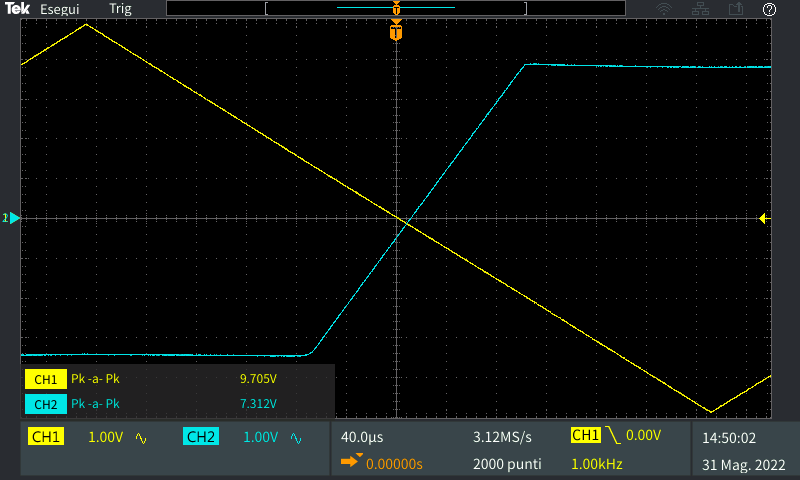
\includegraphics[height=8.9cm]{immagini/oscillo14}
\caption{Grafico della saturazione con un'onda triangolare in ingresso.}
\label{figura:oscillo14}
\end{figure}
\\Dal grafico precedente, si può anche vedere un'altra non-idealità che un amplificatore operazionale reale ha: l'offset in tensione, seppur piccolo, è diverso da 0V. Infatti, il tratto di retta del segnale in uscita non passa per l'origine, ma lo taglia ad un valore poco maggiore di 0V.
\section{Integratore} \label{int_cap}
Se al circuito precedente mettiamo un condensatore in parallelo alla resistenza $R_2$, otteniamo un integratore reale. Di seguito si riportano lo schema, l'analisi del circuito e le misure effettuate su di questo.
\subsection{Schema}
\begin{figure}[h]
\centering
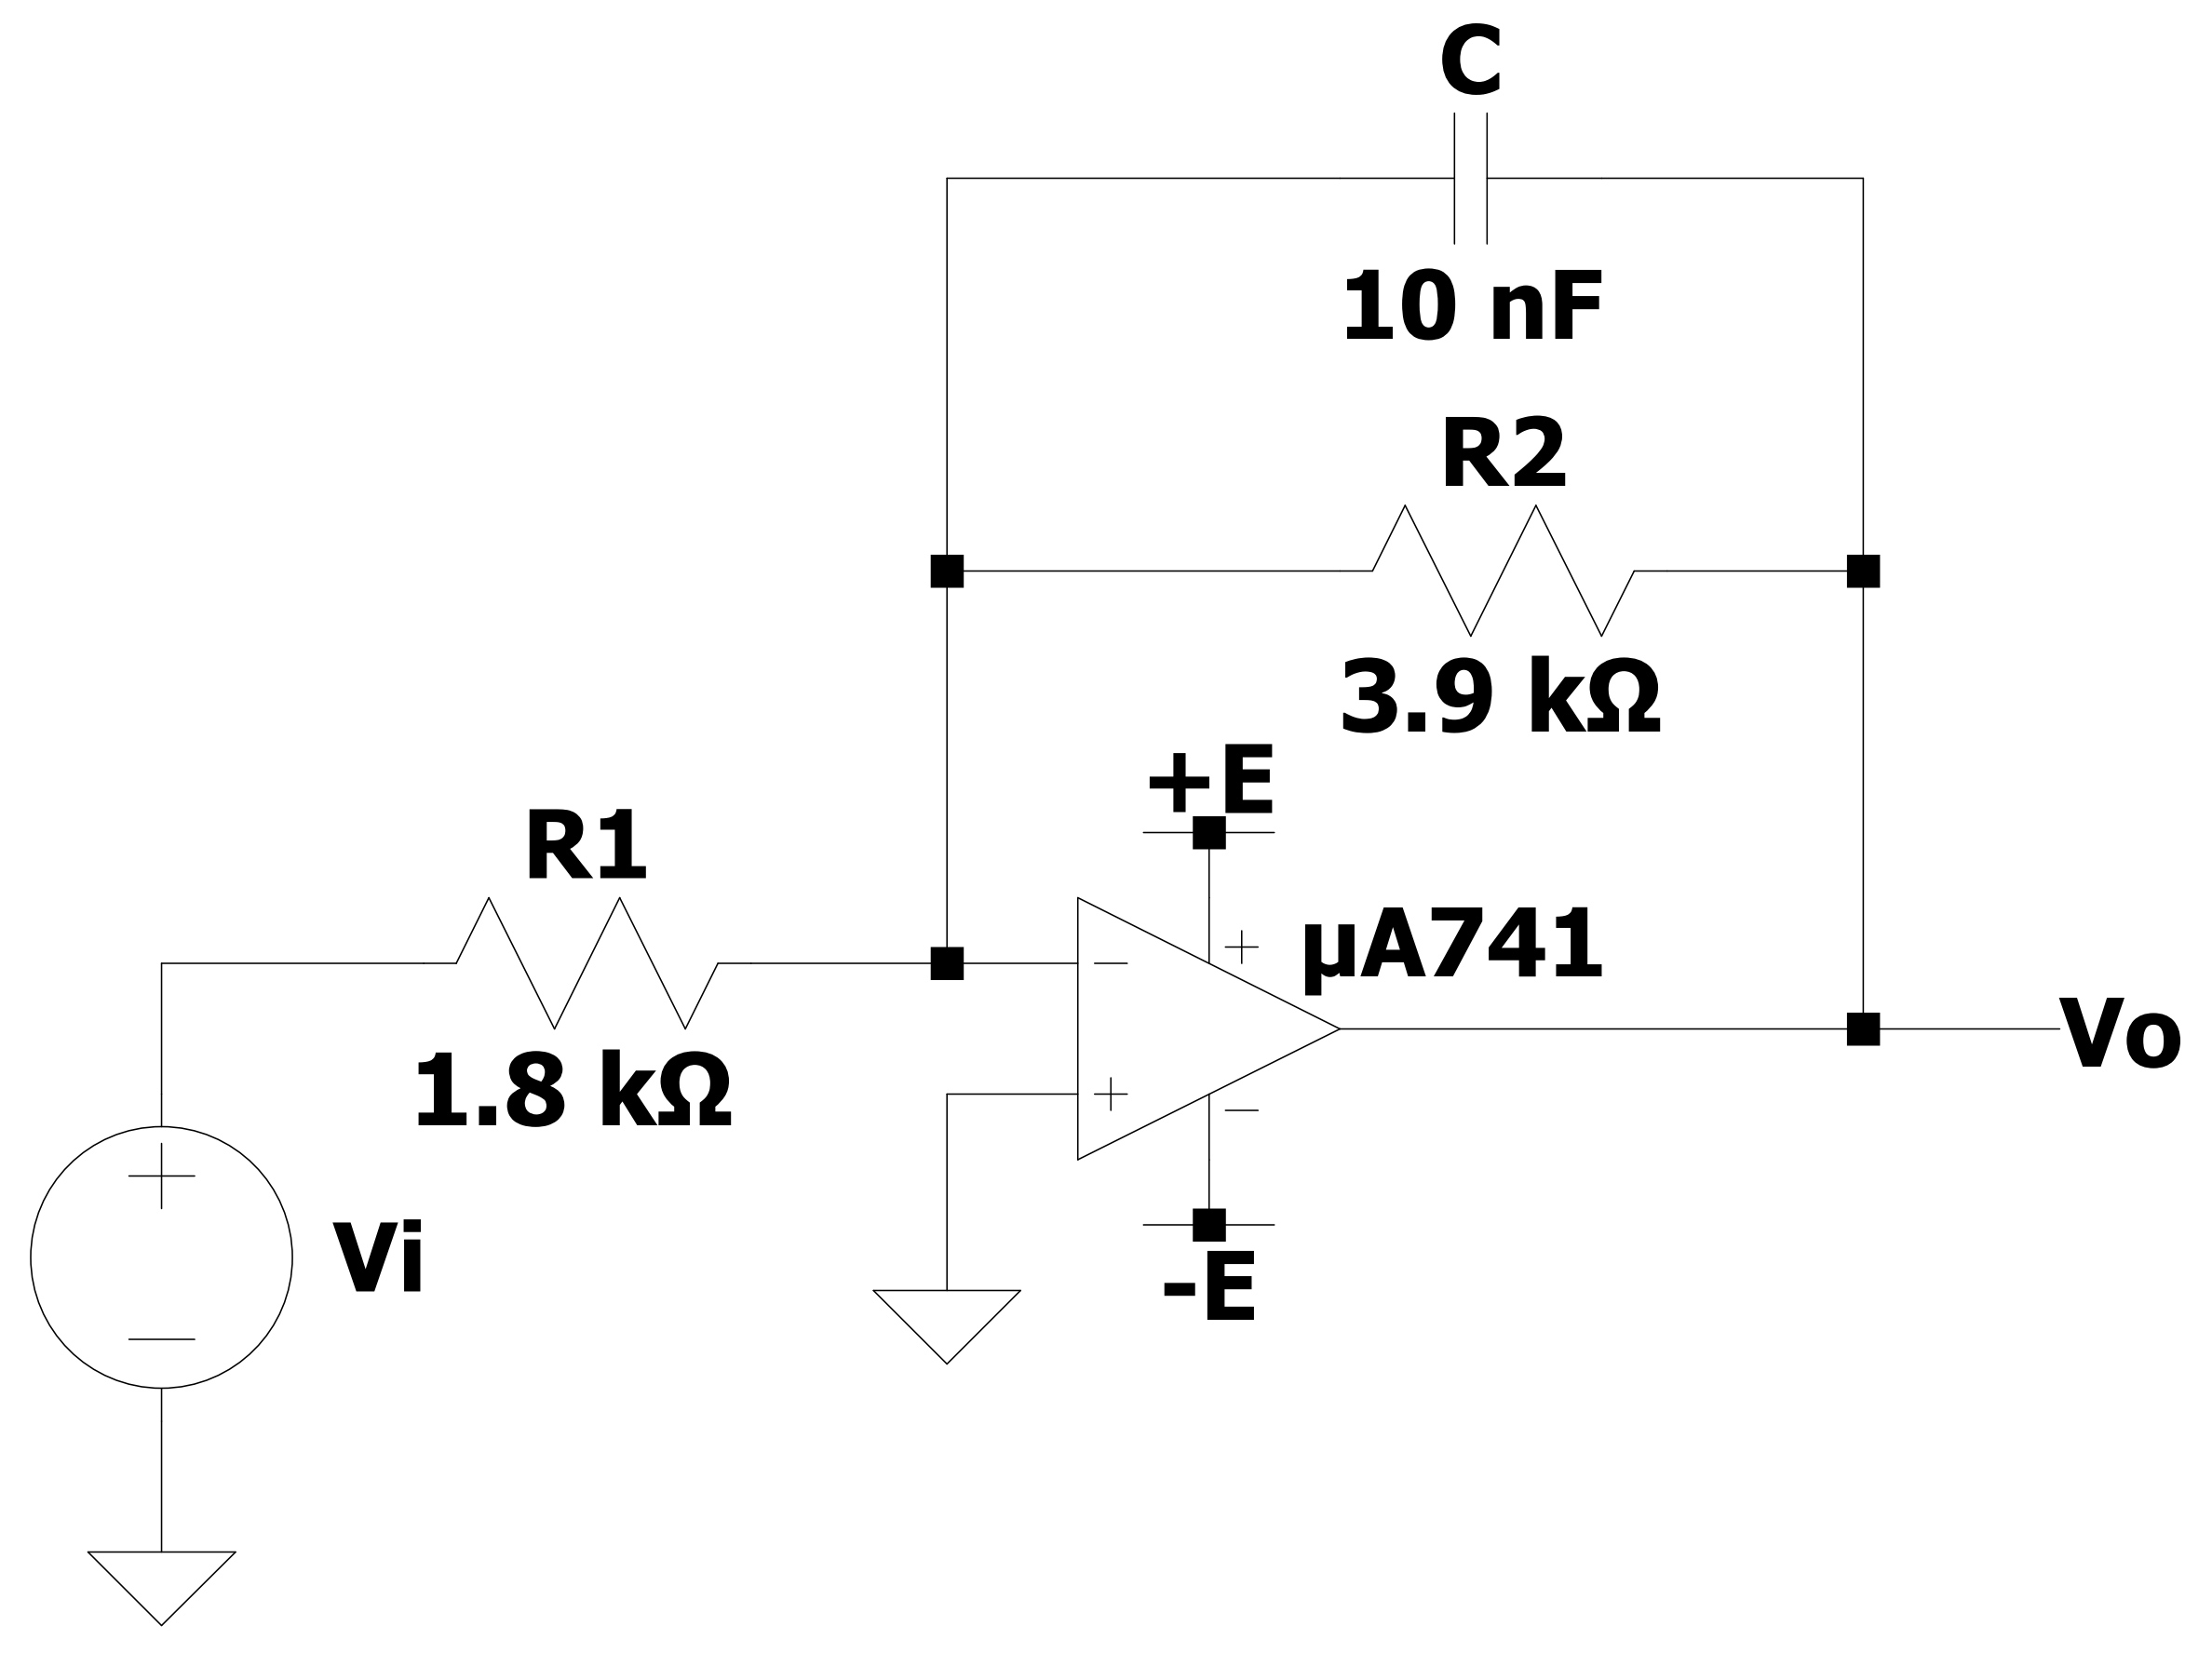
\includegraphics[height=8.2cm]{immagini/int}
\caption{Schema dell'integratore reale.}
\label{figura:int}
\end{figure}
\subsection{Analisi del circuito} 
L'analisi di questo circuito è molto simile a quella dell'amplificatore invertente presentata nella sezione \ref{amplinv_analisi_cap}, solo che per l'integratore dobbiamo esplicitare la dipendenza dalla variabile $s$. Anche in questo caso il circuito è retroazionato negativamente, perché l'uscita viene riportata all'ingresso invertente dell'amplificatore operazionale. 
\\[2pt]La resistenza $R_2$ e il condensatore $C$ sono in parallelo, pertanto si può calcolare l'impedenza equivalente:
\\[2pt]\indent$\displaystyle{Z_{eq}=C\parallelsum R_2=\frac{\frac{1}{s\cdot C} \cdot R_2}{\frac{1}{s\cdot C} + R_2}=\frac{\frac{R_2}{s\cdot C}}{\frac{1+s\cdot R_2C}{s\cdot C}}=\frac{R_2}{1+s\cdot R_2C}}$
\\Per ricavare la funzione di trasferimento del circuito è sufficiente fare un bilancio di correnti all'ingresso invertente. Con $I_2$ si intende la corrente che scorre nell'impedenza equivalente $Z_{eq}$.
\\[2pt]\indent $I_1=I_2+I_{in^-}$
\\[2pt]La corrente in ingresso all'OPAMP è molto piccola, idealmente $I_{in^+}=I_{in^-}\rightarrow 0A$. Perciò l'equazione precedente diventa:
\\\indent $\displaystyle{I_1=I_2}$
\\Utilizzando la legge di Ohm generalizzata, le correnti si possono esprimere come:
\\[2pt]\indent $\displaystyle{\frac{V^-(s)-V_i(s)}{R_1}=(V_o(s)-V^-(s))\cdot\frac{1+s\cdot R_2C}{R2}}$
\\[2pt]Se un circuito è retroazionato negativamente, $V^+=V^-$ per il principio del cortocircuito virtuale. Dato che $V^+$ è a massa, la sua tensione è di 0V, di conseguenza anche $V^-$ si troverà a questa tensione. L'equzione precedente diventa:
\\[2pt]\indent $\displaystyle{\frac{-V_i(s)}{R_1}=V_o(s)\cdot\frac{1+s\cdot R_2C}{R2}}$
\\[2pt]Tramite quest'equazione è facile ricavare la funzione di trasferimento del circuito, che risulta:
\\[2pt]\indent $\displaystyle{\frac{V_o(s)}{V_i(s)}=-\frac{R_2}{R_1}\cdot\frac{1}{1+s\cdot R_2C}}$
\\[2pt]La funzione di trasferimento ottenuta è quella di un filtro passa-basso, perché al denominatore troviamo $1+s\cdot R_2C$. Vediamo che c'è però anche un fattore di guadagno pari al rapporto fra $R_2$ e $R_1$. Compare anche un segno meno, pertanto l'ingresso e l'uscita sono sfasate di 180°
\\Se passiamo al regime sinusoidale, sostituiamo $s$ con $j\omega$. La funzione di trasferimento diventa:
\\[2pt]\indent $\displaystyle{\frac{V_o(\omega)}{V_i(\omega)}=-\frac{R_2}{R_1}\cdot\frac{1}{1+j\omega\cdot R_2C}}$
\\[2pt]Ipotizzando di lavorare ad una frequenza molto maggiore della frequenza di taglio, ovvero se $f\gg f_T$ e quindi $\displaystyle{f\gg \frac{1}{2\pi\cdot R_2C}\simeq\SI{4081}{\hertz}}$, la funzione di trasferimento si può riscrivere come:
\\[2pt]\indent$\displaystyle{v_o(\omega)\simeq-\frac{R_2}{R_1}\cdot\frac{1}{j\omega\cdot R_2C}\cdot v_i(\omega)=-\frac{1}{j\omega R_1C}\cdot v_i(\omega)}$
\\[2pt]Il circuito si chiama integratore perché, se passiamo al dominio del tempo, antitrasformando la funzione di trasferimento, otteniamo:
\\[2pt]\indent$\displaystyle{v_o(t)=-\frac{1}{R_1C}\cdot\int_{0}^{t}v_i(\tau)d\tau}$
\\[2pt]Quindi, l'uscita è l'integrale nel tempo del segnale in ingresso, sfasata di 180°.
\subsection{Componenti, strumenti e misure} 
Il circuito è stato realizzato su una breadboard utilizzando questi componenti:
\begin{itemize}
\item una resistenza da \SI{3.9}{k\ohm} per $R_2$;
\item una resistenza da \SI{1.8}{k\ohm} per $R_1$;
\item un condensatore da \SI{10}{n\farad} per $C$;
\item amplificatore operazionale \textmu A741.
\end{itemize}
Per le misure e le analisi, sono stati utilizzati i seguenti strumenti:
\begin{itemize}
\item alimentatore da banco, con alimentazione positiva impostata a 5V ed alimentazione negativa a -5V, entrambe con limite in corrente di 50mA;
\item generatore di forme d'onda;
\item multimetro da banco;
\item oscilloscopio a due canali.
\end{itemize}
In figura \ref{figura:foto_int} è mostrata una fotografia del circuito in cui possiamo vedere sia dove applichiamo il segnale, che dove colleghiamo le due sonde dell'oscilloscopio. Nella fotografia, il pin numero 1 del \textmu A741 si trova in basso a sinistra.
\begin{figure}[h]
\centering
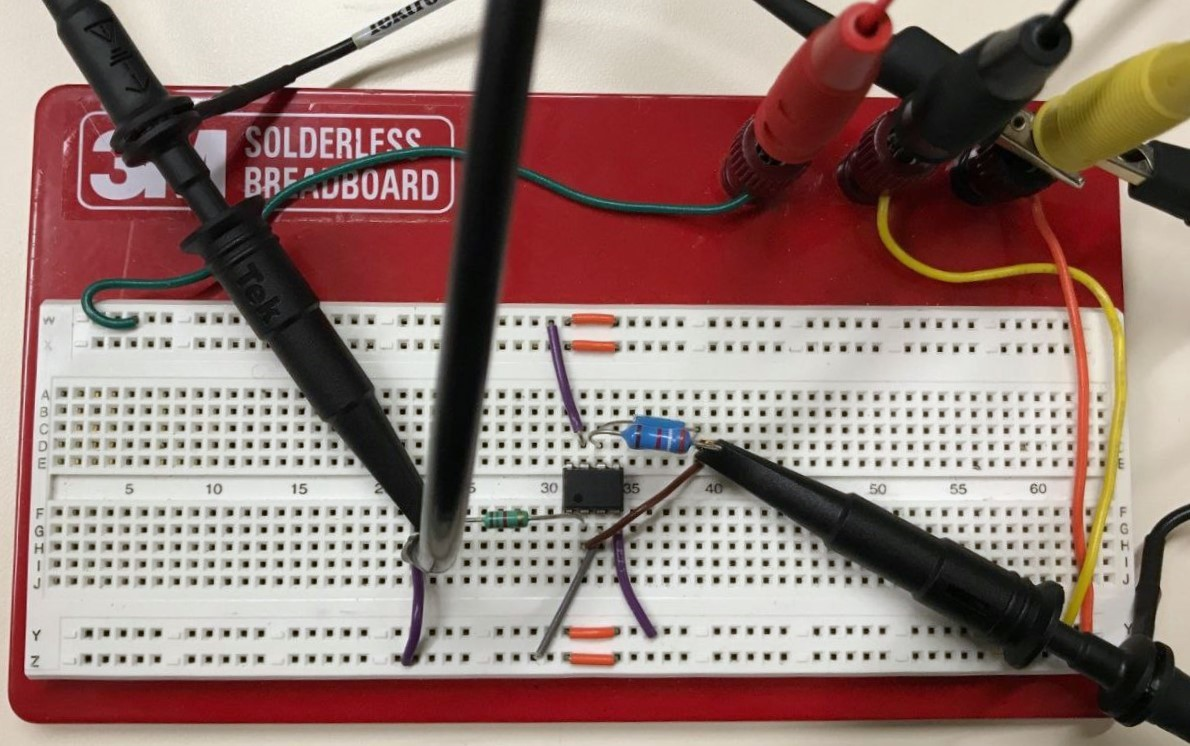
\includegraphics[height=7.2cm]{immagini/foto_int}
\caption{Integratore invertente con \textmu A741.}
\label{figura:foto_int}
\end{figure}
\\Stavolta non effettuiamo delle misure sui componenti del circuito perché utilizziamo quelli dell'amplificatore invertente. I valori sono già stati riportati in tabella \ref{table:amplinv_comp}.
\\\indent Dopo aver posizionato tutti i componenti sulla breadboard, abbiamo applicato il segnale, successivamente abbiamo collegato le sonde dell'oscilloscopio. La forma d'onda utilizzata è un'onda quadra con tensione picco-picco di 1V e frequenza di \SI{100}{k\hertz}. In figura \ref{figura:oscillo15} vediamo il grafico che ci mostra l'oscilloscopio quando in ingresso abbiamo un'onda quadra. Va notato che i picchi dovuti a distrurbi sul segnale d'ingresso sono ancor più visibili in uscita a causa dell'amplificazione. 
\begin{figure}[h!]
\centering
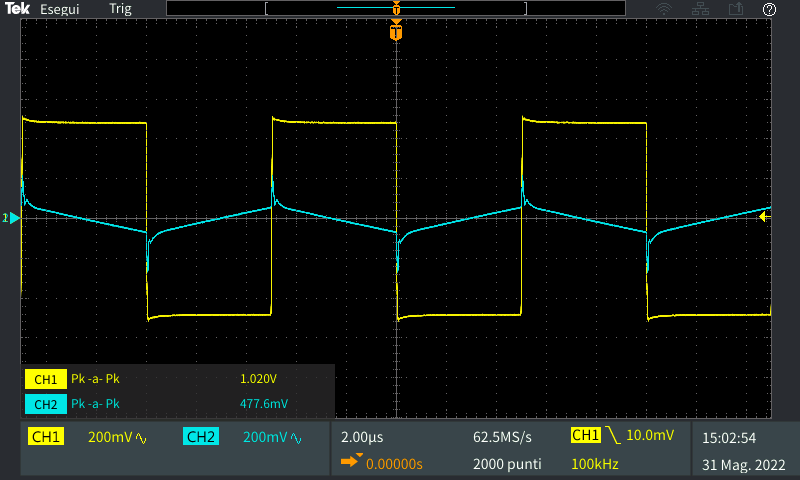
\includegraphics[height=7.2cm]{immagini/oscillo15}
\caption{Grafico della tensione in ingresso e in uscita al circuito integratore.}
\label{figura:oscillo15}
\end{figure}
\\L'onda quadra può essere vista come una funzione costante a tratti:
\begin{equation}
	f(x)=\label{eq1_int}
	\begin{cases}
		0.5\indent\;se\;0\le x<T/2 \\
		-0.5\indent\;se\;T/2\le x<T 
	\end{cases}
\end{equation}
se integriamo questa funzione, otteniamo:
\begin{equation}
	F(x)=\label{eq2_int}
	\begin{cases}
		~0.5\cdot x + cost\indent\;se\;0\le x<T/2 \\
		-0.5\cdot x + cost\indent\;se\;T/2\le x<T 
	\end{cases}
\end{equation}
Questa funzione rappresenta un'onda triangolare, com'è visibile anche dal grafico dell'oscilloscopio. Si può anche notare che lo sfasamento fra ingresso e uscita è di 180°, perché nel semiperiodo in cui l'onda quadra è alta, l'onda triangolare decresce, mentre nel semiperiodo in cui l'onda quadra è bassa, l'onda triangolare cresce. Se l'integratore non fosse invertente, ci aspetteremmo il contrario, ovvero se l'onda quadra è alta, l'onda triangolare cresce, al contrario se l'onda quadra è bassa, l'onda triangolare decresce, in accordo con le funzioni \eqref{eq1_int} e \eqref{eq2_int}.


%----------------------------------------------------------------------------------------

\end{document}
